\documentclass[oneside]{hcmus-report}
\usepackage{codespace}

% Encodings
\usepackage{gensymb,textcomp}

% Better tables
\usepackage{array,longtable,multicol,multirow,siunitx,tabularx}

% Better enum
\usepackage{enumitem}

% Graphics
\usepackage{caption,float,graphicx,subcaption}
\usepackage[export]{adjustbox}
\captionsetup{hypcap=false}

% Math
\usepackage{amsmath,amssymb,amsthm}
\usepackage{mathtools}

% Theorem environments
\theoremstyle{plain}
\newtheorem{theorem}{Định lý}[section]
\newtheorem{lemma}[theorem]{Bổ đề}
\newtheorem{corollary}[theorem]{Hệ quả}
\newtheorem{proposition}[theorem]{Mệnh đề}

\theoremstyle{definition}
\newtheorem{definition}[theorem]{Định nghĩa}
\newtheorem{example}[theorem]{Ví dụ}
\newtheorem{remark}[theorem]{Nhận xét}

\usepackage{caption}
\usepackage{placeins}
\usepackage{tikz}
\usepackage{pgfplots}
\pgfplotsset{compat=1.18}
\usetikzlibrary{angles, quotes, arrows.meta, calc, automata, positioning, fit, shapes.geometric}
\usepackage{xcolor}

\usepackage{pgfplotstable}
\usetikzlibrary{arrows.meta, positioning, shapes.geometric, shapes.misc, fit, backgrounds, calc,decorations.pathreplacing, matrix, patterns}
\usepackage{booktabs}


% Box cho phần [MỞ RỘNG]
\usepackage{tcolorbox}
\tcbuselibrary{breakable,skins}
\newtcolorbox{morong}[1][]{
  colback=yellow!8!white,
  colframe=orange!70!black,
  fonttitle=\bfseries,
  title={\textbf{} #1},
  breakable
}

\usepackage{tcolorbox}
\tcbuselibrary{breakable,skins}

% Hộp ghi chú cam (dùng cho cảnh báo / morong gốc)
\newtcolorbox{morong}[1][]{
  colback=yellow!8!white,
  colframe=orange!70!black,
  fonttitle=\bfseries,
  title={\textbf{} #1},
  breakable
}

% Hộp thông tin xanh dương
\newtcolorbox{InfoBox}[1]{
  colback=blue!5!white,
  colframe=blue!55!black,
  fonttitle=\bfseries,
  title={#1},
  breakable
}

% Hộp ghi chú xanh lá
\newtcolorbox{NoteBox}[1]{
  colback=green!5!white,
  colframe=green!45!black,
  fonttitle=\bfseries,
  title={#1},
  breakable
}

% Hộp cảnh báo vàng
\newtcolorbox{WarningBox}[1]{
  colback=yellow!10!white,
  colframe=orange!80!black,
  fonttitle=\bfseries,
  title={#1},
  breakable
}

% Code listing
\usepackage{listings}

\lstdefinelanguage{Julia}{
  morekeywords={abstract,break,case,catch,const,continue,do,else,elseif,end,export,false,for,function,if,import,in,let,macro,module,mutable,quote,return,struct,true,try,using,while},
  sensitive=true,
  morecomment=[l]{\#},
  morestring=[b]",
}

\lstset{
  language=Python,
  basicstyle=\ttfamily\small,
  keywordstyle=\color{blue}\bfseries,
  commentstyle=\color{gray}\itshape,
  stringstyle=\color{orange!80!black},
  numbers=left,
  numberstyle=\tiny\color{gray},
  numbersep=8pt,
  breaklines=true,
  frame=single,
  showstringspaces=false,
  tabsize=4,
  captionpos=b,
}

% Algorithm
\usepackage[ruled,vlined,linesnumbered]{algorithm2e}
\SetAlgorithmName{Thuật toán}{thuattoan}{Danh sách thuật toán}

% References
\usepackage[nameinlink]{cleveref}
\usepackage{xurl}
\usepackage{hyperref}

% Extra packages
\usepackage{longtable,ltablex}
\keepXColumns
\usepackage{xcolor,colortbl}

% Configurations
\coursename{Nhập môn học máy}
\reporttype{BÁO CÁO ĐỒ ÁN 3}
\title{CÁC BƯỚC TIẾN MỚI TRONG GEOMETRIC MACHINE LEARNING}
\advisor{& ThS. Lê Nhựt Nam &}
\stuname{%
  & 23120195 & Lê Hà Thanh Chương \\
  & 23120197 & Trà Văn Sỹ \\
  & 23120199 & Huỳnh Đức Thịnh \\
  & 23120257 & Bùi Trung Hiếu \\
  & 23120330 & Lê Công Phúc \\
}

% Counter settings
\AtBeginDocument{\counterwithin{lstlisting}{section}}
\AtBeginDocument{\counterwithin{equation}{section}}

% Vietnamese section names
\AtBeginDocument{\renewcommand{\contentsname}{Mục lục}}
\AtBeginDocument{\renewcommand{\listfigurename}{Danh sách các hình}}
\AtBeginDocument{\renewcommand{\listtablename}{Danh sách các bảng}}
\AtBeginDocument{\renewcommand{\tablename}{Bảng}}
\AtBeginDocument{\renewcommand{\figurename}{Hình}}
\AtBeginDocument{\renewcommand{\refname}{Tài liệu tham khảo}}
\AtBeginDocument{\renewcommand{\proofname}{Chứng minh}}

% Layout
\setlength{\headheight}{41pt}
\setlength{\hfuzz}{100pt}
\hbadness=10000
\emergencystretch=2em

% Custom math commands
\newcommand{\R}{\mathbb{R}}
\newcommand{\N}{\mathbb{N}}
\renewcommand{\H}{\mathbb{H}}
\newcommand{\X}{\mathcal{X}}
\newcommand{\inner}[2]{\langle #1, #2 \rangle}
\newcommand{\norm}[1]{\left\| #1 \right\|}
\newcommand{\Tr}{\operatorname{Tr}}

\newcommand{\RKHS}{\mathcal{H}}
\newcommand{\featmap}{\Phi}
\newcommand{\kernel}{k}

% (1) Hai màu dùng cho các hình minh hoạ tự vẽ trong Chương 2
\definecolor{gmlblue}{HTML}{2C5F8E}
\definecolor{gmlorange}{HTML}{B5651D}
 
% (2) Kiểu cột tabularx canh trái + tự xuống dòng (cho 2 bảng trong chương).
%     (tabularx đã được nạp trong main.tex; chỉ cần khai báo thêm cột L.)
\newcolumntype{L}{>{\raggedright\arraybackslash}X}
 
% (3) Macro vẽ "mặt mèo" cho hình minh hoạ bất biến/đẳng biến.
%     Cách dùng: \catface{x}{y}{scale}
\newcommand{\catface}[3]{%
  \begin{scope}[shift={(#1,#2)}, scale=#3]
    \fill[orange!72!yellow]    (-0.42,0.30)--(-0.12,0.74)--(0.02,0.34)--cycle; % tai trái
    \fill[orange!72!yellow]    ( 0.42,0.30)--( 0.12,0.74)--(-0.02,0.34)--cycle;% tai phải
    \fill[orange!45!yellow]    (-0.34,0.36)--(-0.16,0.62)--(-0.04,0.38)--cycle;
    \fill[orange!45!yellow]    ( 0.34,0.36)--( 0.16,0.62)--( 0.04,0.38)--cycle;
    \fill[orange!72!yellow]    (0,0) circle (0.48);
    \fill[black] (-0.18,0.06) circle (0.055);
    \fill[black] ( 0.18,0.06) circle (0.055);
    \fill[pink!80!red] (0,-0.10) ellipse (0.07 and 0.05);
    \draw[black!70, line width=0.3pt] (0,-0.15)--(0,-0.24);
    \draw[black!70, line width=0.3pt] (-0.40,-0.02)--(-0.18,-0.06);
    \draw[black!70, line width=0.3pt] (-0.42,-0.12)--(-0.18,-0.12);
    \draw[black!70, line width=0.3pt] ( 0.40,-0.02)--( 0.18,-0.06);
    \draw[black!70, line width=0.3pt] ( 0.42,-0.12)--( 0.18,-0.12);
  \end{scope}}
  
% (4) Macro vẽ "mặt CHÓ" cho hình minh hoạ Ví dụ 2.3 / 2.4.
%     Cách dùng: \dogface{x}{y}{scale}
\newcommand{\dogface}[3]{%
  \begin{scope}[shift={(#1,#2)}, scale=#3]
    \begin{scope}[shift={(-0.40,0.10)}, rotate=30]
      \fill[brown!55!black] (0,0) ellipse [x radius=0.15, y radius=0.34];
    \end{scope}
    \begin{scope}[shift={(0.40,0.10)}, rotate=-30]
      \fill[brown!55!black] (0,0) ellipse [x radius=0.15, y radius=0.34];
    \end{scope}
    \fill[brown!62!orange] (0,0) circle (0.46);
    \fill[brown!28!white] (0,-0.16) ellipse [x radius=0.27, y radius=0.21];
    \fill[black] (-0.17,0.12) circle (0.052);
    \fill[black] ( 0.17,0.12) circle (0.052);
    \fill[white] (-0.155,0.135) circle (0.016);
    \fill[white] ( 0.185,0.135) circle (0.016);
    \fill[black] (0,0.0) ellipse [x radius=0.085, y radius=0.065];
    \fill[white!75!black] (0.022,0.02) circle (0.012);
    \draw[black!75, line width=0.5pt] (0,-0.065) -- (0,-0.17);
    \draw[black!75, line width=0.5pt] (0,-0.17) .. controls (-0.05,-0.22) and (-0.12,-0.20) .. (-0.16,-0.15);
    \draw[black!75, line width=0.5pt] (0,-0.17) .. controls ( 0.05,-0.22) and ( 0.12,-0.20) .. ( 0.16,-0.15);
    \fill[red!55!pink] (0,-0.205) ellipse [x radius=0.05, y radius=0.07];
  \end{scope}}

% (5) Shortcut màu cho hình Ví dụ 2.6/2.7
\colorlet{c1}{gmlblue}          % xanh  – nút 1 / nguyên tử chính
\colorlet{c2}{gmlorange}        % cam   – nút 2
\colorlet{c3}{green!55!black}   % lục   – nút 3

\begin{document}
\coverpage%

% Đánh số trang La Mã cho phần mở đầu (front matter)
\pagenumbering{roman}

% Mục lục
\tableofcontents

\clearpage
\phantomsection
\addcontentsline{toc}{section}{Danh sách các hình}
\listoffigures

\clearpage
\phantomsection
\addcontentsline{toc}{section}{Danh sách các bảng}
\listoftables

% ==============================================================================
% DANH SÁCH CÁC KÝ HIỆU VÀ CHỮ VIẾT TẮT
% ==============================================================================
\clearpage
\section*{Danh sách các ký hiệu và chữ viết tắt}
\addcontentsline{toc}{section}{Danh sách các ký hiệu và chữ viết tắt}

\begin{longtable}{p{0.25\textwidth} p{0.70\textwidth}}
\textbf{Ký hiệu / Viết tắt} & \textbf{Ý nghĩa} \\
\hline
\endfirsthead

\textbf{Ký hiệu / Viết tắt} & \textbf{Ý nghĩa} (tiếp theo) \\
\hline
\endhead

% ==========================================
% PHẦN 1: CHỮ VIẾT TẮT
% ==========================================
\multicolumn{2}{c}{\textbf{Chữ viết tắt}} \\
\hline
API & Giao diện lập trình ứng dụng (Application Programming Interface) \\
AUC & Diện tích dưới đường cong ROC (Area Under the Curve) \\
CNN & Mạng tích chập (Convolutional Neural Network) \\
DA & Tăng cường dữ liệu (Data Augmentation) \\
DQN & Deep Q-network, thuật toán học tăng cường dựa trên xấp xỉ $Q$-function bằng mạng nơ-ron.\\
FLOPs & Số phép toán dấu phẩy động mỗi giây (Floating Point Operations Per Second) \\
GNN & Mạng nơ-ron đồ thị (Graph Neural Network) \\
KRR & Hồi quy kernel ridge (Kernel Ridge Regression) \\
MDP & Markov decision process, mô hình toán học cho bài toán ra quyết định tuần tự.\\
MLP & Perceptron đa lớp (Multi-Layer Perceptron) \\
MVCNN & Mạng chập đa góc nhìn (Multi-view Convolutional Neural Network) \\
PCA & Phân tích thành phần chính (Principal Component Analysis) \\
RKHS & Không gian Hilbert tái sinh (Reproducing Kernel Hilbert Space) \\
SAC & Soft Actor-Critic, thuật toán actor-critic có entropy regularization.\\
SSL & Học tự giám sát (Self-Supervised Learning) \\

\hline

% ==========================================
% PHẦN 2: KÝ HIỆU
% ==========================================

% --- Nhóm 1: Không gian, tập hợp và cấu trúc hình học ---
\multicolumn{2}{c}{\textbf{Không gian, tập hợp và cấu trúc hình học}} \\
\hline
$\mathbb{R}$ & Tập hợp các số thực \\
$(M, g)$ & Đa tạp Riemann compact, liên thông, không biên với metric $g$ \\
$\mathcal{X}$ & Không gian dữ liệu / không gian đầu vào \\
$\mathcal{Y}$ & Không gian đầu ra của mô hình \\
$\mathcal{H}$ & Không gian Hilbert tái sinh của kernel Sobolev \\
$H^s_{\mathrm{inv}}(M)$ & Không gian Sobolev bậc $s$ gồm các hàm bất biến trên $M$ \\
$M/G$ & Không gian thương gồm các quỹ đạo $[x] = \{\tau(x) : \tau \in G\}$ \\
$\mathrm{Orb}_G(x)$ & Quỹ đạo của $x$ dưới tác động của $G$: tập $\{g \cdot x \mid g \in G\}$ \\
$\mathcal{P}_n$ & Tập các ma trận hoán vị kích thước $n$ \\
$\mathcal{F}(X)$ & Tập hợp khung (Frame) trích xuất từ điểm dữ liệu $X$ \\

\hline

% --- Nhóm 2: Nhóm đối xứng và tác động nhóm ---
\multicolumn{2}{c}{\textbf{Nhóm đối xứng và tác động nhóm}} \\
\hline
$G$ & Nhóm đối xứng; trong Chương 4 là compact Lie group tác động trơn, đẳng cự lên $M$ \\
$G$ & Group đối xứng tác động lên state và action.\\
$g \in G$ & Phần tử nhóm, đại diện cho một phép biến đổi \\
$g$ & Một phần tử thuộc group $G$.\\
$g \cdot x$ & Tác động của phần tử $g$ lên điểm dữ liệu $x$ \\
$S_n$ & Nhóm hoán vị $n$ phần tử \\
$C_n, C_4$ & Nhóm xoay tuần hoàn; $C_4$ gồm bốn phép quay cách nhau $90^\circ$ \\
$SO(d)$ & Nhóm quay đặc biệt trong $\mathbb{R}^d$ \\
$SO(2)$ & Nhóm các phép xoay trong mặt phẳng.\\
$SE(2), SE(3)$ & Nhóm Euclid đặc biệt trong 2D/3D, gồm quay và tịnh tiến \\
$SE(2)$ & Nhóm các phép tịnh tiến và xoay trong mặt phẳng.\\
$SE(3)$ & Nhóm các phép tịnh tiến và xoay trong không gian ba chiều.\\
$E(3)$ & Nhóm Euclidean trong $\mathbb{R}^3$ (quay, phản xạ, tịnh tiến) \\
$GL(V)$ & Nhóm các ánh xạ tuyến tính khả nghịch trên không gian vector $V$ \\

\hline

% --- Nhóm 3: MDP, state, action và robotics ---
\multicolumn{2}{c}{\textbf{MDP, state, action và robotics}} \\
\hline
$\mathcal{M}$ & Markov decision process biểu diễn bài toán ra quyết định của robot.\\
$\mathcal{S}$ & State space của MDP.\\
$\mathcal{A}$ & Action space của MDP.\\
$\mathcal{T}$ & Transition function của MDP.\\
$\mathcal{R}$ & Reward function của MDP.\\
$\gamma$ & Discount factor trong MDP.\\
$s$ & State của robot hoặc môi trường.\\
$a$ & Action của robot.\\
$g \cdot s$ & State sau khi chịu tác động của phép biến đổi $g$.\\
$g \cdot a$ & Action sau khi chịu tác động của phép biến đổi $g$.\\
$\pi^*$ & Optimal policy.\\
$Q^*$ & Optimal action-value function.\\
$V^*$ & Optimal value function.\\

\hline

% --- Nhóm 4: Toán tử, hàm số và phép toán ---
\multicolumn{2}{c}{\textbf{Toán tử, hàm số và phép toán}} \\
\hline
$f$ & Mô hình hoặc hàm ánh xạ từ đầu vào sang đầu ra \\
$T, T'$ & Phép biến đổi trên không gian đầu vào và phép biến đổi tương ứng trên không gian đầu ra \\
$\tau_v$ & Phép tịnh tiến theo vector $v$ \\
$P$ & Ma trận hoán vị dùng để đánh số lại phần tử hoặc nút \\
$P_\sigma$ & Ma trận hoán vị biểu diễn hoán vị $\sigma$ \\
$\rho, \rho(g)$ & Biểu diễn nhóm, ánh xạ phần tử nhóm thành phép biến đổi tuyến tính \\
$\rho_1, \rho_2$ & Biểu diễn nhóm (group representations) \\
$K(x, y)$ & Hàm hạt nhân đánh giá giữa hai điểm $x$ và $y$ \\
$f_{\star}$ & Hàm mục tiêu bất biến / hàm sinh nhãn thật \\
$\hat{f}$ & Hàm ước lượng học được từ dữ liệu huấn luyện \\
$\eta$ & Tham số điều chuẩn trong hồi quy kernel ridge \\
$\mathrm{vol}(M/G)$ & Thể tích của không gian thương $M/G$ \\
$T_a, R_a$ & Phép biến đổi tuyến tính trong không gian ẩn tương ứng với phép tăng cường $a$ \\
$A$ & Ma trận biến đổi afin dự đoán bởi mạng học sâu (ví dụ T-Net) \\
$c(x)$ & Dạng chuẩn (canonical form) của điểm dữ liệu $x$ \\
$\mathcal{L}$ & Hàm mất mát (loss function) \\
$\langle \Phi \rangle_G$ & Phép toán lấy trung bình nhóm (Group averaging) \\
$\langle \Phi \rangle_{\mathcal{F}}$ & Phép toán lấy trung bình khung (Frame averaging) \\
$L_{reg}$ & Hàm mất mát chính quy hóa (regularization loss) \\

\hline

% --- Nhóm 5: Biến số, chỉ số và ký hiệu Hy Lạp ---
\multicolumn{2}{c}{\textbf{Biến số, chỉ số và ký hiệu Hy Lạp}} \\
\hline
$n, N$ & Số lượng phần tử hoặc số lượng điểm đầu vào \\
$\alpha$ & Biên an toàn (margin) / Giới hạn độ tin cậy / Ngưỡng kiểm soát tỷ lệ lỗi \\
$d' = \dim(M) - \dim(G)$ & Số chiều hiệu dụng sau khi loại bỏ bậc tự do đối xứng \\
$\epsilon_i$ & Nhiễu quan sát của mẫu thứ $i$ \\
$\sigma^2$ & Phương sai của nhiễu quan sát \\
$\sigma$ & Một hoán vị, thường là phần tử của nhóm hoán vị $S_n$ \\

\hline
\end{longtable}

\clearpage
\phantomsection

\section*{Danh mục các thuật ngữ}
\addcontentsline{toc}{section}{Danh mục các thuật ngữ}

\begin{longtable}{p{0.44\textwidth} p{0.46\textwidth}}
\textbf{Thuật ngữ tiếng Anh} & \textbf{Thuật ngữ tiếng Việt} \\
\hline
\endfirsthead
\textbf{Thuật ngữ tiếng Anh} & \textbf{Thuật ngữ tiếng Việt} \\
\hline
\endhead

Absolute convergence & Hội tụ tuyệt đối \\
Accepting path & Đường đi chấp nhận \\
Affine transformation & Phép biến đổi afin \\
Canonical form / Canonicalization & Dạng chuẩn / Chuẩn hóa \\
Compact Lie group & Nhóm Lie compact \\
Commutative diagram & Sơ đồ giao hoán \\
Contrastive learning & Học tương phản \\
Critical points & Điểm tới hạn \\
Cyclic group & Nhóm tuần hoàn \\
Data augmentation & Tăng cường dữ liệu \\
Equivariance & Đẳng biến / tương biến \\
Euclidean group & Nhóm Euclid \\
Frame averaging & Lấy trung bình khung \\
Generator (of a group) & Tập sinh (của một nhóm) \\
Graph isomorphism & Đẳng cấu đồ thị \\
Grasp learning & Bài toán học cách xác định và thực hiện thao tác gắp vật thể.\\
Group & Nhóm (đại số) \\
Group action & Tác động nhóm \\
Group averaging / Reynolds operator & Lấy trung bình nhóm / Toán tử Reynolds \\
Group representation & Biểu diễn nhóm \\
Invariance & Bất biến (invariance) \\
Latent space & Không gian ẩn \\
Max pooling & Gộp cực đại \\
Monte Carlo & Phương pháp Monte Carlo \\
Orbit & Quỹ đạo \\
Orthogonal matrix & Ma trận trực giao \\
Partially equivariant model & Mô hình chỉ áp dụng equivariance cho một phần state hoặc action phù hợp với đối xứng của bài toán.\\
Permutation group & Nhóm hoán vị \\
Point cloud & Đám mây điểm \\
Quotient space & Không gian thương \\
Reproducing kernel Hilbert space & Không gian Hilbert tái sinh \\
Representer theorem & Định lý biểu diễn nghiệm \\
Representation learning & Học biểu diễn \\
Riemannian manifold & Đa tạp Riemann \\
Robot manipulation & Bài toán điều khiển robot tương tác vật lý với vật thể.\\
Robust frames & Khung bền vững \\
Rotation group & Nhóm xoay \\
Sample-efficient learning & Khả năng học được chính sách tốt với ít dữ liệu hoặc ít lần tương tác hơn.\\
Self-supervised learning & Học tự giám sát \\
Set equivariance & Tương biến tập hợp \\
Sobolev space & Không gian Sobolev \\
Spatial action space & Action space có cấu trúc không gian, thường gắn với vị trí, hướng hoặc pose.\\
Spectral averaging & Lấy trung bình phổ \\
Symmetry & Tính đối xứng \\
Symmetry function & Hàm đối xứng \\
Translation group & Nhóm tịnh tiến \\
Universal approximation & Xấp xỉ phổ quát \\
Weighted frame & Khung có trọng số \\

\end{longtable}

\clearpage

% Reset về số Ả Rập từ trang 1 bắt đầu từ Chương 1
\pagenumbering{arabic}
\section*{Lời mở đầu}
\addcontentsline{toc}{section}{Lời mở đầu}

Đồ án của nhóm tập trung vào 

\clearpage

\section{Giới thiệu}
\label{sec:gioi-thieu}

\subsection{Bối cảnh và động lực thực hiện}
\label{subsec:boi-canh}

Trong thập kỷ qua, sự thành công của các mô hình học sâu trong việc giải quyết những bài toán phức tạp của trí tuệ nhân tạo là điều không thể phủ nhận. Tuy nhiên, sự phát triển này lại đi kèm với những thách thức to lớn về mặt lý thuyết và thực tiễn, đặt ra yêu cầu cấp thiết về một khung toán học thống nhất và sự hiểu biết sâu sắc hơn về bản chất của các mô hình nơ-ron nhân tạo.

\subsubsection{Vấn đề phân mảnh kiến trúc và lời nguyền đa chiều}
\label{subsubsec:phan-manh-kien-truc}

Hạn chế đầu tiên và rõ rệt nhất của lĩnh vực học sâu hiện đại là sự thiếu vắng các nguyên lý thống nhất. Hiện nay, cộng đồng nghiên cứu đang chứng kiến sự bùng nổ của vô số kiến trúc mạng nơ-ron khác nhau, được thiết kế riêng biệt cho từng định dạng dữ liệu. Sự phân mảnh này dẫn đến tình trạng các khái niệm cơ bản liên tục được phát minh lại và định danh dưới những tên gọi khác nhau trong các lĩnh vực ứng dụng riêng biệt, làm lu mờ đi bản chất toán học cốt lõi của bài toán.

Bên cạnh đó, dưới góc độ lý thuyết học thống kê, việc xấp xỉ một hàm số tổng quát trong không gian đa chiều mà không dựa trên bất kỳ giả định tiên nghiệm nào là một bài toán bị chi phối nặng nề bởi lời nguyền đa chiều. Nếu chỉ dựa trên giả định về tính trơn cục bộ, độ phức tạp mẫu yêu cầu để học chính xác hàm mục tiêu sẽ tăng theo cấp số nhân so với số chiều của dữ liệu, khiến bài toán trở nên bất khả thi trong thực tế ngay cả với năng lực tính toán hiện đại.

\begin{infobox}{Khai thác tiên nghiệm hình học phá vỡ lời nguyền đa chiều}
Tuy nhiên, dữ liệu trong thế giới thực hiếm khi tồn tại dưới dạng các vector vô hướng ngẫu nhiên; chúng luôn mang theo những quy luật vật lý và cấu trúc hình học đặc thù, chẳng hạn như tính chu kỳ trong tín hiệu, cấu trúc lưới trong hình ảnh, hoặc các liên kết tô-pô trong phân tử hóa học. Việc khai thác các tiên nghiệm hình học này, đặc biệt là tính bất biến và tính đẳng biến thông qua lăng kính của \textit{Geometric Deep Learning}, đóng vai trò như một cơ chế lọc tự nhiên, giúp giới hạn triệt để không gian hàm cần tìm kiếm, qua đó trực tiếp phá vỡ lời nguyền đa chiều và cung cấp một bản thiết kế chung để hệ thống hóa toàn bộ các kiến trúc mạng hiện hành như CNN, RNN và GNN.
\end{infobox}

\subsubsection{Tính đối xứng tham số và học không gian trọng số}
\label{subsubsec:doi-xung-tham-so}

Sự chuyển dịch bối cảnh thứ hai xuất phát từ chính cấu trúc bên trong của các mô hình ngôn ngữ và mô hình tạo sinh quy mô lớn hiện nay. Các mô hình học sâu hiện đại có đặc điểm chung là bị siêu tham số hóa, dẫn đến sự suy biến nghiêm trọng trong không gian tối ưu: có vô số cấu hình trọng số khác nhau nhưng lại sản sinh ra cùng một hàm tính toán ở đầu ra.

Tính dôi dư này bắt nguồn từ tính đối xứng không gian tham số. Khác với đối xứng của dữ liệu đầu vào trong \textit{Geometric Deep Learning} truyền thống, đối xứng tham số là những phép biến đổi áp dụng trực tiếp lên các ma trận trọng số mà không làm thay đổi hành vi của toàn bộ mạng. Sự tồn tại của các đa tạp chứa điểm cực tiểu tương đương này định hình cấu trúc của cảnh quan hàm mất mát, gây ra các hiện tượng như sự kết nối cực tiểu và làm phức tạp hóa quá trình tối ưu hóa.

\begin{morong}[Xu hướng học không gian trọng số trong kỷ nguyên mô hình nền tảng]
Với sự bùng nổ của hàng triệu mô hình được lưu trữ trên các nền tảng mã nguồn mở, cộng đồng đang chứng kiến một hệ quả tất yếu là sự ra đời của hướng nghiên cứu học không gian trọng số. Hướng đi này coi chính các kiến trúc mạng nơ-ron là dữ liệu đầu vào, sử dụng \textit{meta-networks} để phân tích, nén và tinh chỉnh trực tiếp trên cấu trúc tham số. Trong kỷ nguyên của mô hình nền tảng, việc hiểu và tận dụng các đối xứng tham số linh hoạt thay vì \textit{hard-coding} trở thành chìa khóa để cải thiện định luật tỷ lệ và tăng cường hiệu quả tính toán.
\end{morong}

\subsubsection{Ý nghĩa và tầm quan trọng thực tiễn}
\label{subsubsec:y-nghia-thuc-tien}

Sự kết hợp giữa lý thuyết hình học của dữ liệu và tính đối xứng trong không gian tham số mang lại những bước tiến mang tính bản lề cho toàn bộ vòng đời của hệ thống học máy. Về mặt lý thuyết toán học, các chứng minh mới nhất cho thấy việc mã hóa tính đối xứng giúp cải thiện mạnh mẽ độ phức tạp mẫu, giảm thiểu nhu cầu dữ liệu lên đến nhiều bậc độ lớn, và gia tăng khả năng tổng quát hóa ngoài phân phối một cách nghiêm ngặt.

\begin{importantbox}{Ứng dụng khoa học mũi nhọn trong thế giới thực}
Hơn thế nữa, các mô hình học sâu dựa trên nền tảng hình học và đối xứng đang đóng vai trò trung tâm trong việc giải quyết những bài toán khoa học mũi nhọn. Từ việc mô phỏng hệ nguyên tử, dự đoán năng lượng tương tác phân tử, đến việc ứng dụng tính đẳng biến nhóm $SE(3)$ trong Robotics để điều khiển thao tác trong không gian vật lý, \textit{Geometric Deep Learning} đang chứng minh tiềm năng to lớn trong việc định hình các hệ thống trí tuệ nhân tạo có khả năng tương tác trực tiếp với các định luật vật lý của thế giới thực.
\end{importantbox}

\subsection{Kỷ nguyên của dữ liệu hình học}
\label{subsec:ky-nguyen-du-lieu-hinh-hoc}

Lĩnh vực học máy đang chứng kiến nỗ lực to lớn nhằm hợp nhất các mô hình phân mảnh thành một hệ thống lý thuyết chặt chẽ. Đóng góp nền tảng mang tính bước ngoặt cho nỗ lực này là công trình nghiên cứu \textit{Geometric Deep Learning: Grids, Groups, Graphs, Geodesics, and Gauges} của Bronstein và cộng sự (2021) \cite{bronstein2021geometric}. Hệ thống lý thuyết này được truyền cảm hứng sâu sắc từ chương trình Erlangen của nhà toán học Felix Klein, trong đó đề xuất rằng hình học nên được nghiên cứu thông qua các thuộc tính được bảo toàn dưới tác động của các nhóm phép biến đổi.

Nghiên cứu của Bronstein và cộng sự đã định hình lại cách các hệ thống trí tuệ nhân tạo tiếp nhận dữ liệu. Thay vì xử lý dữ liệu như các vector vô hướng, phương pháp này mô hình hóa dữ liệu dưới dạng các tín hiệu nằm trên năm miền hình học cơ bản, được hệ thống hóa thành khung 5G bao gồm Grids, Groups, Graphs, Geodesics và Gauges. Việc gắn kết dữ liệu vào các miền hình học cụ thể cho phép khai thác triệt để các quy luật tự nhiên, chẳng hạn như tính chu kỳ của ảnh trên miền Grids hay liên kết hóa học trên miền Graphs.

\begin{center}
    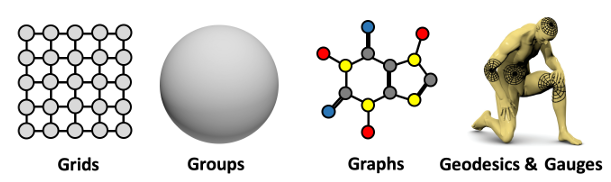
\includegraphics[width=0.85\textwidth, keepaspectratio]{graphics/5g_framework.png}
    
    \vspace{0.2cm}
    \captionof{figure}{Phân loại các miền hình học theo khung 5G}
    \label{fig:5g-framework}
\end{center}
\noindent\textit{Ghi chú: Các miền hình học cơ bản bao gồm Grids, Groups, Graphs, Geodesics và Gauges. Nguồn: \textit{Geometric Deep Learning: Grids, Groups, Graphs, Geodesics, and Gauges} (Bronstein et al., 2021).}

Từ sự phân loại này, một bản thiết kế chung được đề xuất nhằm chuẩn hóa cấu trúc của mạng nơ-ron. Cấu trúc này bao gồm bốn thành phần tính toán cốt lõi: lớp đồng biến tuyến tính, hàm kích hoạt phi tuyến, lớp gộp cục bộ để trích xuất đặc trưng đa tỷ lệ, và lớp gộp bất biến toàn cục ở cuối mạng. Trong đó, hai khái niệm toán học đóng vai trò nền tảng là Invariance và Equivariance. Invariance đảm bảo đầu ra của mô hình không thay đổi khi dữ liệu đầu vào bị biến đổi, trong khi Equivariance yêu cầu đầu ra phải biến thiên một cách tương ứng theo đúng phép biến đổi của đầu vào.

\begin{center}
    \begin{tikzpicture}[node distance=3.5cm, auto, thick, >=Stealth]
        % Sơ đồ Equivariance (Trái)
        \node (X) at (0, 0) {$\mathcal{X}$};
        \node (Y) at (3, 0) {$\mathcal{Y}$};
        \node (TX) at (0, -2.5) {$\mathcal{X}$};
        \node (TY) at (3, -2.5) {$\mathcal{Y}$};
        \draw[->] (X) -- node {$f$} (Y);
        \draw[->] (X) -- node[swap] {$\mathfrak{g}$} (TX);
        \draw[->] (Y) -- node {$\mathfrak{g}'$} (TY);
        \draw[->] (TX) -- node[swap] {$f$} (TY);
        
        \node[below=0.5cm of TX, xshift=1.5cm] {\textbf{(a) Equivariance}};

        % Sơ đồ Invariance (Phải)
        \node (X2) at (6, 0) {$\mathcal{X}$};
        \node (Y2) at (9, -1.25) {$\mathcal{Y}$};
        \node (TX2) at (6, -2.5) {$\mathcal{X}$};
        \draw[->] (X2) -- node {$f$} (Y2);
        \draw[->] (X2) -- node[swap] {$\mathfrak{g}$} (TX2);
        \draw[->] (TX2) -- node[swap] {$f$} (Y2);

        \node[below=0.5cm of TX2, xshift=1.5cm] {\textbf{(b) Invariance}};
    \end{tikzpicture}
    
    \vspace{0.2cm}
    \captionof{figure}{Sơ đồ giao hoán toán học}
    \label{fig:commutative-diagram}
\end{center}
\noindent\textit{Ghi chú: (a) Tính đẳng biến (Equivariance): Biến đổi đầu vào tương đương với việc áp dụng phép biến đổi tương ứng lên đầu ra. (b) Tính bất biến (Invariance): Đầu ra không bị ảnh hưởng bởi phép biến đổi nhóm $\mathfrak{g}$.}

Bản thiết kế này cung cấp một khuôn khổ toán học minh bạch, chứng minh rằng các kiến trúc thành công nhất hiện nay như CNN, RNN, GNN và Transformer thực chất chỉ là các biến thể khác nhau của cùng một nguyên lý đối xứng khi áp dụng lên các miền dữ liệu hình học khác nhau.

\subsection{Sự dịch chuyển sang không gian trọng số}
\label{subsec:su-dich-chuyen-khong-gian-trong-so}

Nếu như giai đoạn đầu của Geometric Deep Learning tập trung giải quyết các bài toán liên quan đến đối xứng trong không gian dữ liệu, thì xu hướng nghiên cứu hiện đại đang chứng kiến một bước chuyển dịch chiến lược. Sự dịch chuyển này được khảo sát và hệ thống hóa một cách toàn diện trong nghiên cứu \textit{Symmetry in Neural Network Parameter Spaces} do Zhao và cộng sự (2026) thực hiện \cite{zhao2026symmetry}. Nhóm tác giả đã chuyển hướng phân tích trọng tâm từ dữ liệu đầu vào sang việc khám phá tính đối xứng nằm ngay bên trong cấu trúc tham số của mạng nơ-ron (Parameter space symmetry).

Theo phân tích của Zhao và cộng sự, các mô hình học sâu hiện đại thường ở trạng thái siêu tham số hóa, dẫn đến hiện tượng vô số cấu hình trọng số khác nhau nhưng lại sản sinh ra cùng một hàm tính toán ở đầu ra. Sự dư thừa này bắt nguồn từ các phép biến đổi nội tại, chẳng hạn như hoán vị các nơ-ron ẩn hoặc thay đổi tỷ lệ trọng số của hàm kích hoạt ReLU, mà không làm thay đổi giá trị dự đoán cuối cùng. Việc nhận diện Parameter space symmetry giúp giải mã cấu trúc phức tạp của Loss landscape, giải thích nguyên nhân hình thành các vùng bình nguyên và hiện tượng Mode connectivity giữa các điểm cực tiểu cục bộ.

\begin{morong}[Kỹ thuật Teleportation và Equivariant Metanetworks]
Khám phá này mở ra những kỹ thuật tối ưu hóa đột phá, điển hình là phương pháp Teleportation, cho phép thuật toán Gradient Descent chủ động dịch chuyển tham số đến các cấu hình tương đương mang đặc tính hội tụ tốt hơn. Quan trọng hơn, sự hiểu biết về đối xứng tham số là tiền đề cho lĩnh vực Weight space learning. Trong mô hình này, các tập hợp trọng số được xem như dữ liệu đầu vào cho một hệ thống Equivariant Metanetworks. Kiến trúc cấp cao này có khả năng dự đoán khả năng tổng quát hóa, nén mô hình và hợp nhất các điểm cực tiểu một cách hiệu quả mà không cần tiến hành suy luận trực tiếp trên dữ liệu gốc.
\end{morong}

\subsection{Mục tiêu và phạm vi của đồ án}
\label{subsec:muc-tieu-va-pham-vi}

\subsubsection{Mục tiêu nghiên cứu}
\label{subsubsec:muc-tieu-nghien-cuu}

Đồ án này hướng tới việc hệ thống hóa và thực nghiệm các kỹ thuật tiên tiến nhất trong lĩnh vực học máy hình học, dựa trên nền tảng lý thuyết từ các hội nghị đầu ngành. Việc tích hợp các tiên nghiệm hình học vào mô hình nhằm chứng minh ba lợi ích cốt lõi sau:

\begin{itemize}
    \item \textbf{Giảm bậc tự do và tăng Data efficiency:} Bằng cách ràng buộc không gian tìm kiếm thông qua các phép đối xứng, mô hình có thể đạt được độ chính xác cao với lượng dữ liệu huấn luyện ít hơn nhiều bậc độ lớn so với các phương pháp truyền thống.
    \item \textbf{Cải thiện OOD generalization và Robustness:} Kiến trúc tôn trọng các phép biến đổi hình học giúp hệ thống duy trì tính ổn định và khả năng ngoại suy chính xác khi đối mặt với dữ liệu nằm ngoài phân phối huấn luyện ban đầu.
    \item \textbf{Hỗ trợ các tác vụ tạo sinh:} Hiểu rõ cơ chế duy trì và phá vỡ đối xứng cung cấp nền tảng toán học vững chắc cho việc thiết kế các mô hình tạo sinh cấu trúc phức tạp như phân tử thuốc hay protein.
\end{itemize}

\subsubsection{Phạm vi và cấu trúc báo cáo}
\label{subsubsec:pham-vi-cau-truc}

Báo cáo tổng hợp các kỹ thuật từ nền tảng toán học cơ bản đến những hướng tiếp cận mới nhất về đối xứng tham số và học không gian trọng số. Nội dung chi tiết được tổ chức thành năm chương tiếp theo:

\begin{itemize}
    \item \textbf{Chương 2} trình bày kiến thức nền tảng toán học, tập trung vào lý thuyết nhóm, tính bất biến và tính đẳng biến.
    \item \textbf{Chương 3} phân tích các phương pháp cốt lõi để xây dựng mô hình tương biến, bao gồm các phép tích chập nhóm và cơ chế chia sẻ tham số.
    \item \textbf{Chương 4} mở rộng sang các kỹ thuật xử lý dữ liệu hiện đại như Frame averaging và các lý thuyết mới về học không gian trọng số.
    \item \textbf{Chương 5} mô tả chi tiết thiết lập thực nghiệm, cấu hình phần cứng và phân tích kết quả so sánh giữa mô hình đề xuất và các phương pháp cơ sở.
    \item \textbf{Chương 6} tổng hợp các đánh giá ưu nhược điểm, rút ra kết luận về tính ứng dụng thực tiễn và định hướng các nghiên cứu trong tương lai.
\end{itemize}

\clearpage
\section{Kiến thức nền tảng}
\label{sec:kien-thuc-nen}

% ============================================================
% MỤC TIÊU CHƯƠNG:
% Cung cấp nền tảng toán học tối thiểu cần thiết để hiểu
% toàn bộ các phương pháp ở Chương 3 và 4.
% Nguồn: Slides Part 1 (Groups, Group Actions, Representations)
% ============================================================

\subsection{Đối xứng và vai trò trong học máy}
\label{subsec:doi-xung}
% Trình bày: Symmetry là gì? Ví dụ trực quan trong thực tế
% (ảnh phân loại, đám mây điểm, đồ thị, neural networks).
% Tại sao encoding symmetry giúp: fewer degrees of freedom,
% data efficiency, OOD generalization.
% Dẫn nguồn: NequIP (3 bậc ít data hơn), scaling laws.

\subsection{Tính Bất biến và Tính Đẳng biến}
\label{subsec:invariance-equivariance}
% Trình bày:
%   - Invariance: f(T(x)) = f(x)
%   - Equivariance: f(T(x)) = T(f(x))
%   - Sơ đồ giao hoán (commutative diagram)
%   - Invariance là trường hợp đặc biệt của Equivariance
%     (scalar output, transformation = identity)
% Ví dụ: shift/rotation invariance trong image classification,
%   permutation equivariance trong node embedding.

\subsection{Lý thuyết Nhóm cơ bản}
\label{subsec:group-theory}
% Trình bày:
%   - Group G: 4 tính chất (associativity, identity, inverse, closure)
%   - Ví dụ: S_n (permutations), SO(3) (rotations), C_n (cyclic/shift),
%     E(3) (Euclidean: rotation + reflection + translation)
%   - Group action: G acts on X as g.x
%   - Group representation: biểu diễn g bằng ma trận ρ(g),
%     yêu cầu ρ(gh) = ρ(g)ρ(h)
%   - Orbit: Orb_G(x) = {g.x | g ∈ G}

\subsection{Biểu diễn nhóm và ý nghĩa với kiến trúc mạng}
\label{subsec:group-representation}
% Trình bày:
%   - Regular vs. irreducible representations
%   - Schur's Lemma (dẫn dắt tới hạn chế của equivariant linear layers
%     ở Chương 3, mục Tensor Methods)
%   - Fourier analysis trên groups (dẫn dắt tới Expanders ở Chương 4)
% Chú ý: không cần quá sâu, mục tiêu là cung cấp vocabulary
%   cho các chương sau.

\clearpage
\section{Các phương pháp xây dựng mô hình bảo toàn tính đối xứng}
\label{sec:phuong-phap}

% ============================================================
% MỤC TIÊU CHƯƠNG:
% Trình bày 2 hướng chính để đưa tính đối xứng vào AI,
% cùng các ứng dụng thực tế và giới hạn của chúng.
% Nguồn: Slides Part 1 (trang 15–55), Tutorial Part 1
% ============================================================

% ─────────────────────────────────────────────────────────────
% HƯỚNG 1: CAN THIỆP DỮ LIỆU (OFF-THE-SHELF MODELS)
% Dùng model bình thường + xử lý dữ liệu đầu vào/đầu ra
% để đạt được tính invariance/equivariance.
% ─────────────────────────────────────────────────────────────

\subsection{Hướng 1: Can thiệp dữ liệu trên các mô hình có sẵn}
\label{subsec:off-the-shelf}

Trước khi đi vào các phương pháp xây dựng kiến trúc hoàn toàn mới, một hướng tiếp cận tự nhiên hơn là tận dụng lại những mô hình học máy đã được huấn luyện tốt (thứ mà cộng đồng nghiên cứu đã đổ rất nhiều công sức phát triển) rồi can thiệp vào phía dữ liệu để ép mô hình phải tôn trọng tính đối xứng. Hướng này được gọi là hướng can thiệp dữ liệu, hay còn được gọi là cách tiếp cận với mô hình hộp đen.

Ưu điểm cốt lõi của hướng này là mô hình cơ sở (dù là Transformer, CNN hay bất kỳ kiến trúc nào khác) được giữ nguyên hoàn toàn, kéo theo toàn bộ sức mạnh biểu diễn, kỹ thuật tối ưu, và quy trình huấn luyện của nó vẫn còn hiệu lực. Điều đó có nghĩa là người dùng không cần thiết kế lại bất cứ điều gì từ đầu. Ngoài ra, nếu mô hình cơ sở đã có sẵn một số tính chất đối xứng nhất định, việc kết hợp thêm các nhóm đối xứng khác thông qua can thiệp dữ liệu là hoàn toàn khả thi mà không gây mâu thuẫn.

Trong hướng này có ba kỹ thuật chính: tăng cường dữ liệu, chuẩn hóa, và lấy trung bình nhóm/khung. Ba kỹ thuật này nằm trên một phổ liên tục: từ một phép biến đổi duy nhất ở một đầu, đến lấy trung bình trên toàn bộ nhóm $G$ ở đầu kia, với lấy trung bình khung nằm ở giữa như một điểm cân bằng giữa chi phí tính toán và chất lượng đảm bảo tính đối xứng.

\subsubsection{Tăng cường dữ liệu}
\label{subsubsec:data-augmentation}

\paragraph{Ý tưởng cơ bản.}
Tăng cường dữ liệu là kỹ thuật đơn giản và phổ biến nhất để đưa tính đối xứng vào mô hình: với mỗi điểm dữ liệu $x$ trong tập huấn luyện, ta sinh thêm các biến thể $g \cdot x$ cho nhiều phần tử $g \in G$ khác nhau và đưa chúng vào tập huấn luyện cùng nhãn gốc. Khi tập huấn luyện bao phủ đủ nhiều biến thể của quỹ đạo $\mathrm{Orb}_G(x)$, mô hình sẽ dần học được rằng phép biến đổi $g$ không làm thay đổi nhãn, tức là dần hình thành tính bất biến.

Kỹ thuật này cực kỳ linh hoạt vì nó có thể áp dụng cho cả học có giám sát lẫn học tự giám sát. Trong học tương phản, người ta thường tạo cặp dữ liệu $(x, g \cdot x)$ và đặt chúng ở vị trí ``dương'' (positive pair), buộc mô hình phải đặt cả hai vào cùng một vùng trong không gian ẩn. Qua đó, toàn bộ quỹ đạo của $x$ dưới tác động của $G$ sẽ được ánh xạ về một biểu diễn duy nhất.

\paragraph{Giới hạn: chỉ đảm bảo tính đối xứng xấp xỉ.}
Dù đơn giản và hiệu quả trong thực tế, tăng cường dữ liệu mang một hạn chế quan trọng về mặt lý thuyết: nó không đảm bảo tính bất biến ở mọi điểm. Sau khi huấn luyện, không có gì chắc chắn rằng với một điểm dữ liệu mới $x'$ chưa thấy, mô hình sẽ cho ra cùng một kết quả cho $x'$ và $g \cdot x'$. Mô hình có thể đã \textit{học ước lượng} tính bất biến trong vùng lân cận của dữ liệu huấn luyện, nhưng không có gì đảm bảo điều đó khái quát hóa ra ngoài phân phối.

\begin{warningbox}{Tăng cường dữ liệu chỉ đưa ra xấp xỉ, không phải bảo đảm}
Biểu hiện thực tế của hạn chế này: mô hình huấn luyện với tăng cường dữ liệu thường hoạt động tốt trên bộ test trong phân phối, nhưng rất dễ bị đánh lừa khi gặp các đầu vào bị biến đổi ở góc độ chưa từng xuất hiện trong tập huấn luyện. Đây không phải lỗi do lượng dữ liệu ít, mà là một giới hạn căn bản: không có đảm bảo tính bất biến ở mọi nơi.
\end{warningbox}

\paragraph{Mở rộng: học biểu diễn equivariant.}
Một bước phát triển thú vị từ tăng cường dữ liệu là học biểu diễn \textit{equivariant} thay vì chỉ invariant. Trong bài toán học biểu diễn, đôi khi ta không muốn hoàn toàn ``quên đi'' phép biến đổi mà dữ liệu đã trải qua; ta muốn không gian ẩn ghi nhớ lại sự biến đổi đó theo một cách có cấu trúc. Cụ thể, nếu $a$ là một phép tăng cường và $f$ là mạng mã hóa, thì mục tiêu là:
\begin{equation}
    f(a(x)) = T_a \cdot f(x),
\end{equation}
trong đó $T_a$ là một phép biến đổi tác động lên không gian ẩn, tương ứng với $a$. Đây chính là định nghĩa equivariance áp dụng vào bài toán học biểu diễn. Hình~\ref{fig:equivariant-repr} minh họa trực quan ý tưởng này.

\begin{figure}[H]
    \centering
    \begin{tikzpicture}[
        node distance=2.2cm and 3.8cm
        every node/.style={font=\normalsize},
        box/.style={draw, rounded corners=4pt, minimum width=1.5cm, minimum height=0.8cm,,
                    fill=blue!8, thick},
        arr/.style={->, >=Stealth, thick, blue!60!black}
    ]
        \node[box] (x)  {$x$};
        \node[box] (ax) [right=of x]  {$a(x)$};
        \node[box] (fx) [below=of x]  {$f(x)$};
        \node[box] (fax)[below=of ax] {$f(a(x))$};

        \draw[arr] (x)  -- node[above]{augmentation $a$} (ax);
        \draw[arr] (x)  -- node[left] {encoder $f$}      (fx);
        \draw[arr] (ax) -- node[right]{encoder $f$}      (fax);
        \draw[arr] (fx) -- node[below]{transform $T_a$}  (fax);

        \node[font=\footnotesize, align=center] at (1.9,-1.1)
            {\textit{both paths}\\[2pt]\textit{yield the same result}};
    \end{tikzpicture}
    \caption{Sơ đồ giao hoán của học biểu diễn equivariant: áp dụng phép tăng cường $a$ rồi mã hóa, hoặc mã hóa rồi tác động $T_a$ trong không gian ẩn, đều cho cùng kết quả.}
    \label{fig:equivariant-repr}
\end{figure}

Một cách tiếp cận trực tiếp là dùng một mạng nhỏ $\mathrm{MLP}(a, f(x))$ để dự đoán $f(a(x))$, từ đó đặt hàm mất mát:
\begin{equation}
    \mathcal{L} = \bigl\| f(a(x)) - \mathrm{MLP}(a,\, f(x)) \bigr\|.
\end{equation}
Tuy nhiên, cách này có một nhược điểm: không có gì đảm bảo $T_a$ sẽ tương thích với phép kết hợp nhóm, tức là $T_{a_2 \circ a_1} \neq T_{a_2} \circ T_{a_1}$ có thể xảy ra.

\paragraph{Phiên bản tuyến tính: ràng buộc bảo toàn tích vô hướng.}
Để khắc phục hạn chế đó, các nghiên cứu sau này đề xuất một cách đơn giản hơn: giả định rằng $T_a$ là một phép quay tác động lên không gian ẩn, tức là $T_a = R_a$ là ma trận trực giao. Khi đó, ta không cần trực tiếp học $R_a$, mà thay vào đó tận dụng tính chất của phép quay: nó bảo toàn tích vô hướng giữa hai vector. Cụ thể, nếu $f(a(x'))^\top f(a(x)) = f(x')^\top f(x)$ với mọi cặp $(x, x')$ và phép tăng cường $a$, thì $T_a$ nhất thiết phải là một phép quay. Hàm mất mát tương ứng là:
\begin{equation}
    \mathbb{E}_{a,\, x,\, x'} \left[ f(a(x'))^\top f(a(x)) - f(x')^\top f(x) \right]^2 = 0.
\end{equation}

Khi hàm mất mát bằng 0, mỗi $T_a = R_a$ là một phép quay trong không gian ẩn và tự động tương thích với phép kết hợp nhóm --- tức là $\{T_a\}_{a \in G}$ tạo thành một biểu diễn nhóm của $G$. Điều đáng chú ý là phép tăng cường $a$ tác động lên đầu vào không nhất thiết phải là một phép quay; đây là hệ quả của định lý Peter--Weyl trong lý thuyết nhóm. Hướng này được phát triển bởi Shakerinava et al.\ (2022) và Gupta et al.\ (2023).

\subsubsection{Chuẩn hóa}
\label{subsubsec:canonicalization}

\paragraph{Ý tưởng cơ bản.}
Kỹ thuật chuẩn hóa theo đuổi một chiến lược hoàn toàn khác: thay vì làm phong phú tập dữ liệu bằng nhiều biến thể, ta chuyển mỗi điểm dữ liệu $x$ về một dạng chuẩn duy nhất trước khi đưa vào mô hình. Miễn là hàm chuẩn hóa $c(\cdot)$ ánh xạ mọi phần tử trong cùng một quỹ đạo về cùng một điểm duy nhất, thì mô hình sẽ tự động bất biến:
\begin{equation}
    c(g \cdot x) = c(x) \quad \forall\, g \in G.
\end{equation}

Ví dụ điển hình nhất là sắp xếp cho bài toán invariant với hoán vị: với bất kỳ chuỗi nào, ta sắp xếp nó theo thứ tự tăng dần trước khi đưa vào mô hình. Vì mọi hoán vị của cùng một chuỗi đều cho ra cùng một dạng đã sắp xếp, mô hình luôn nhận cùng một đầu vào và cho ra cùng một kết quả. Để đạt equivariance thay vì chỉ invariance, ta thực hiện thêm một bước: sau khi mô hình xử lý dạng chuẩn, ta áp dụng phép biến đổi ngược để khôi phục thứ tự ban đầu. Hình~\ref{fig:canon-pipeline} minh họa toàn bộ quy trình này.

\begin{figure}[H]
    \centering
    \begin{tikzpicture}[
        node distance=0.5cm and 1.4cm,
        every node/.style={font=\small},
        box/.style={draw, rounded corners=4pt, minimum width=2.0cm, minimum height=0.75cm,
                    fill=orange!10, thick, align=center},
        op/.style={draw, circle, minimum size=0.7cm, fill=green!15, thick, font=\footnotesize},
        arr/.style={->, >=Stealth, thick}
    ]
        \node[box] (x)      {$x$\\(đầu vào)};
        \node[op]  (c)      [right=of x]          {$c(\cdot)$};
        \node[box] (cx)     [right=of c]          {$c(x)$\\(dạng chuẩn)};
        \node[op]  (f)      [right=of cx]         {$f$};
        \node[box] (fcx)    [right=of f]          {$f(c(x))$\\(đầu ra $f$)};
        \node[op]  (inv)    [right=of fcx]        {$c^{-1}$};
        \node[box] (out)    [right=of inv]        {đầu ra\\equivariant};

        \draw[arr] (x)   -- (c);
        \draw[arr] (c)   -- (cx);
        \draw[arr] (cx)  -- (f);
        \draw[arr] (f)   -- (fcx);
        \draw[arr] (fcx) -- (inv);
        \draw[arr] (inv) -- (out);

        % Invariant path (shorter)
        \draw[arr, dashed, gray] (fcx.south) -- ++(0,-0.6)
            node[below, align=center, font=\footnotesize, gray]
            {nếu chỉ cần invariance:\\dừng ở đây};
    \end{tikzpicture}
    \caption{Pipeline chuẩn hóa: đầu vào $x$ được ánh xạ về dạng chuẩn $c(x)$, xử lý bằng mô hình $f$, sau đó áp dụng phép biến đổi ngược $c^{-1}$ để đạt equivariance. Nếu chỉ cần invariance thì bỏ qua bước cuối.}
    \label{fig:canon-pipeline}
\end{figure}

Trong ví dụ sắp xếp, nếu dãy $[5,\, 3,\, 4]$ được sắp thành $[3,\, 4,\, 5]$, mô hình xử lý và cho ra kết quả theo thứ tự đó, rồi ta hoán vị ngược lại để đầu ra có thứ tự tương ứng với đầu vào gốc.

Hàm chuẩn hóa $c(\cdot)$ không nhất thiết phải được thiết kế bằng tay; nó cũng có thể được học từ dữ liệu thông qua một mạng neural phụ trợ \cite{kaba2022equivariance}. Hướng này mở ra khả năng tận dụng sức mạnh của deep learning để tự động tìm ra cách biểu diễn chuẩn phù hợp nhất cho bài toán cụ thể.

\paragraph{Thách thức 1: không phải lúc nào cũng dễ xác định dạng chuẩn.}
Đối với chuỗi số, sắp xếp là một lựa chọn tự nhiên và đơn giản. Nhưng không phải mọi loại dữ liệu đều có một dạng chuẩn rõ ràng. Hãy lấy ví dụ với đồ thị: một đồ thị $n$ nút có thể được mô tả bởi $n!$ ma trận kề khác nhau, tương ứng với $n!$ cách đánh số các nút. Tìm một biểu diễn chuẩn chung cho tất cả các cách đánh số đó về cơ bản tương đương với việc giải bài toán kiểm tra đẳng cấu đồ thị (graph isomorphism) --- một bài toán đã được nghiên cứu trong nhiều thập kỷ nhưng vẫn chưa có thuật toán đa thức được chứng minh. Tương tự với đám mây điểm trong không gian 3D kết hợp đối xứng quay và hoán vị, việc chuẩn hóa trở nên rất phức tạp.

\paragraph{Thách thức 2: vấn đề tính liên tục.}
Đây là hạn chế lý thuyết nghiêm trọng nhất của kỹ thuật chuẩn hóa. Tính liên tục yêu cầu rằng nếu hai đầu vào gần nhau thì hai đầu ra cũng phải gần nhau. Với chuỗi số vô hướng, sắp xếp duy trì tính liên tục vì một thay đổi nhỏ thường không làm đảo lộn toàn bộ thứ tự. Tuy nhiên, câu chuyện hoàn toàn khác khi dữ liệu là các vector đa chiều.

Hãy xem xét ví dụ cụ thể từ slides của khóa học (trang 14 trong file slides NeurIPS 2025): ta có hai đám mây điểm gần nhau, mỗi đám gồm hai vector. Đám thứ nhất chứa $[5,\, 3,\, 3]^\top$ và $[1,\, 7,\, 8]^\top$; đám thứ hai chứa $[5,\, 3.01,\, 3]^\top$ và $[1,\, 7,\, 8]^\top$ --- chỉ thay đổi một phần tử nhỏ từ $3$ thành $3.01$. Nếu ta sắp xếp các vector theo thứ tự từ điển, thì thứ tự sắp xếp của hai đám sẽ khác nhau hoàn toàn vì $3.01$ khiến thứ tự tương đối của hai chiều thứ hai và thứ ba bị đảo ngược. Kết quả là hai đầu vào cực kỳ gần nhau lại được ánh xạ đến hai dạng chuẩn rất xa nhau về khoảng cách Euclidean.
\begin{figure}[H]
    \centering
    \includegraphics[width=0.85\textwidth, keepaspectratio]{graphics/canon_continuity.png}
    \caption{Minh họa vấn đề tính liên tục trong chuẩn hóa: hai đám mây điểm chỉ khác nhau rất nhỏ (số 3 so với 3.01) nhưng sau khi sắp xếp lại cho ra hai dạng chuẩn xa nhau về khoảng cách Euclidean. Nguồn: \cite{jegelka2025tutorial}, trang 14.}
    \label{fig:canon-continuity}
\end{figure}

Kết quả lý thuyết của Dym et al.\ (2024) và Zhang et al.\ (2020) chỉ ra rằng đây không phải vấn đề của riêng một cách sắp xếp cụ thể nào, mà là một giới hạn căn bản không thể tránh được:

\begin{theorem}[Không tồn tại chuẩn hóa liên tục, Dym et al.\ 2024]
\label{thm:no-continuous-canon}
Không tồn tại hàm chuẩn hóa liên tục nào cho nhóm hoán vị $S_n$ tác động lên $\mathbb{R}^{d \times n}$ với $n, d > 1$. Tương tự, không tồn tại frame hữu hạn liên tục nào cho $SO(2)$ trong trường hợp tổng quát.
\end{theorem}

Hệ quả thực tiễn của định lý này là: dù ta thiết kế hàm chuẩn hóa khéo léo đến đâu, sẽ luôn tồn tại những cặp đầu vào gần nhau nhưng có dạng chuẩn cách xa nhau, dẫn đến hành vi không ổn định của mô hình. Đây là lý do frame averaging --- sẽ được trình bày ở mục tiếp theo --- trở thành một lựa chọn hấp dẫn hơn: bằng cách lấy trung bình trên nhiều phép biến đổi thay vì chỉ chọn một, frame averaging khắc phục được vấn đề liên tục này.

\paragraph{Tổng kết về chuẩn hóa.}
Nhìn chung, chuẩn hóa là kỹ thuật hiệu quả và rẻ về tính toán so với lấy trung bình nhóm, đặc biệt khi nhóm $G$ lớn. Nó phù hợp nhất trong các trường hợp dạng chuẩn tự nhiên và dễ xác định (như sắp xếp cho hoán vị trên vô hướng), và cần thận trọng với các bài toán yêu cầu tính ổn định cao trước các nhiễu nhỏ. Bảng~\ref{tab:symmetrization-compare} ở cuối mục này tóm tắt so sánh ba kỹ thuật.

\subsubsection{Lấy trung bình Nhóm và Khung (Group/Frame Averaging)}
\label{subsubsec:frame-averaging}
% ĐÂY LÀ PHẦN CỦA SỸ — Paper 3: Frame Averaging (Puny et al 2022)

% Group Averaging (Reynolds operator):
%   - Invariant: f̄(x) = (1/|G|) Σ_{g∈G} f(g^{-1}·x)
%   - Equivariant: f̄(x) = (1/|G|) Σ_{g∈G} g·f(g^{-1}·x)
%   - Universal approximation (Yarotsky 2021)
%   - Ví dụ: Janossy pooling (Murphy et al 2019),
%     SignNet cho sign flips của eigenvectors (Lim et al 2023)
%   - Nhược điểm: expensive khi |G| lớn → cần approximation

% Frame Averaging (Puny et al 2022):
%   - Thay vì average trên toàn bộ G, chỉ average trên F(X) ⊂ G
%   - F(X) được trích xuất từ data, phải thỏa F(g·X) = g·F(X)
%   - Công thức: ⟨Φ⟩_F(X) = (1/|F(X)|) Σ_{g∈F(X)} ρ₂(g)Φ(ρ₁(g)^{-1}X)
%   - Ví dụ PCA Frame cho point clouds/proteins:
%     F(X) = {(α₁v₁,...,αdvd, t) | αᵢ ∈ {-1,+1}} (sign flips của eigenvectors)
%     Đạt E(3)/SE(3) equivariance với chi phí thấp

% Bảng so sánh 3 phương pháp:
%   Canonicalization:  cheap, NOT continuous
%   Frame Averaging:   cheaper than full, continuous
%   Group Averaging:   most expensive, continuous, universal

% Nội dung đã có trong file gốc (công thức LaTeX của Văn Sỹ)
% — giữ nguyên và mở rộng phần này.

Một trong những phương pháp mạnh mẽ nhất để trang bị tính bất biến (invariance) hoặc tương biến (equivariance) cho một mô hình học máy thông thường là sử dụng toán tử Reynolds, hay còn gọi là kỹ thuật lấy trung bình nhóm (Group Averaging). Cụ thể, cho một mạng nơ-ron cơ sở $\Phi$, ta có thể tạo ra một hàm tương biến $\langle \Phi \rangle_G$ bằng cách tính trung bình đầu ra của $\Phi$ trên toàn bộ các phép biến đổi $g$ thuộc nhóm đối xứng $G$:
\begin{equation}
    \langle \Phi \rangle_G(X) = \frac{1}{|G|} \sum_{g \in G} \rho_2(g)\Phi(\rho_1(g)^{-1}X)
\end{equation}
Mặc dù phương pháp này đảm bảo tính đối xứng tuyệt đối và bảo toàn khả năng biểu diễn của mô hình cơ sở, nó vấp phải trở ngại cực lớn về độ phức tạp tính toán khi nhóm $G$ quá lớn hoặc có số phần tử vô hạn (ví dụ: nhóm hoán vị $S_n$ hoặc nhóm phép quay $SO(3)$).

Để giải quyết bài toán tính toán này, kỹ thuật \textbf{Frame Averaging (Trung bình hóa Khung)} đã được đề xuất \cite{puny2022frame}. Thay vì tính trung bình trên toàn bộ nhóm $G$, phương pháp này chỉ thực hiện lấy trung bình trên một tập hợp con nhỏ $\mathcal{F}(X) \subset G$ được gọi là ``khung'' (frame). Tập hợp $\mathcal{F}(X)$ này được trích xuất dựa trên chính đặc trưng của dữ liệu đầu vào $X$. Để đảm bảo tính tương biến, khung $\mathcal{F}$ phải thỏa mãn điều kiện $\mathcal{F}(\rho_1(g)X) = g\mathcal{F}(X)$. Khi đó, công thức xấp xỉ trở thành:
\begin{equation}
    \langle \Phi \rangle_{\mathcal{F}}(X) = \frac{1}{|\mathcal{F}(X)|} \sum_{g \in \mathcal{F}(X)} \rho_2(g)\Phi(\rho_1(g)^{-1}X)
\end{equation}

\textbf{Ứng dụng PCA Frame cho Đám mây điểm (Point Clouds):}
Trong thực tiễn, đối với dữ liệu không gian 3 chiều như đồ thị phân tử hoặc đám mây điểm, Phân tích thành phần chính (PCA) thường được sử dụng để xây dựng khung. Thuật toán tính tâm của đám mây điểm và trích xuất các vector riêng (eigenvectors) từ ma trận hiệp phương sai. Khi dữ liệu đầu vào bị xoay hoặc tịnh tiến, PCA Frame tự động tính phép xoay ngược để chiếu dữ liệu về canonical frame trước khi đưa qua mạng. Phương pháp này đạt tính bất biến với $E(3)$ với chi phí tính toán cực kỳ thấp.

\subsection{Hướng 2: Xây dựng kiến trúc tương biến từ đầu}
\label{subsec:constructed}

Nếu Hướng 1 xem mô hình học máy như một hộp đen và truyền đạt tính đối xứng từ bên ngoài thông qua thao tác dữ liệu, thì Hướng 2 lựa chọn con đường triệt để hơn: mã hóa cứng tính đối xứng vào chính kiến trúc của mạng. Mô hình tương biến được xây dựng theo cấu trúc tổng quát sau.

\begin{figure}[H]
\centering
\begin{tikzpicture}[>=Stealth, thick]
    % Khai báo các node với khoảng cách mép cố định (sử dụng thư viện positioning)
    \node[draw, rounded corners, fill=blue!10, minimum width=1.2cm, minimum height=0.8cm] (x) {$x$};
    \node[draw, rounded corners, fill=orange!20, minimum height=0.8cm, right=0.6cm of x] (L1) {Lớp tương biến $L_1$};
    \node[draw, rounded corners, fill=gray!15, minimum width=1.5cm, minimum height=0.8cm, right=0.6cm of L1] (sig) {$\sigma(\cdot)$};
    \node[draw, rounded corners, fill=orange!20, minimum height=0.8cm, right=0.6cm of sig] (L2) {Lớp tương biến $L_2$};
    \node[draw, rounded corners, fill=green!20, minimum height=0.8cm, right=0.6cm of L2] (pool) {Gộp bất biến};
    \node[draw, rounded corners, fill=red!10, minimum width=1.2cm, minimum height=0.8cm, right=0.6cm of pool] (y) {$y$};

    % Vẽ mũi tên
    \draw[->] (x) -- (L1);
    \draw[->] (L1) -- (sig);
    \draw[->] (sig) -- (L2);
    \draw[->] (L2) -- (pool);
    \draw[->] (pool) -- (y);

    % Ghi chú bên dưới các khối
    \node[below=0.2cm of L1, font=\small, text=orange!70!black] {tương biến};
    \node[below=0.2cm of L2, font=\small, text=orange!70!black] {tương biến};
    \node[below=0.2cm of pool, font=\small, text=green!60!black] {bất biến};
\end{tikzpicture}
\caption{Cấu trúc tổng quát của mô hình tương biến: xen kẽ các lớp tuyến tính tương biến với hàm kích hoạt phi tuyến $\sigma$, kết thúc bằng một lớp gộp bất biến toàn cục.}
\label{fig:equivariant-pipeline}
\end{figure}

\textbf{Ưu điểm cốt lõi của hướng này:}
\begin{itemize}
    \item Tính đối xứng được đảm bảo tuyệt đối tại mọi điểm dữ liệu, kể cả những điểm chưa thấy trong quá trình huấn luyện.
    \item Số tham số giảm mạnh do cơ chế chia sẻ, dẫn đến hiệu quả dữ liệu cao hơn.
    \item Đặc biệt phù hợp khi tính đối xứng là điều chắc chắn về mặt vật lý hoặc toán học (phân tử, robot, đồ thị).
\end{itemize}

% ──────────────────────────────────────────────────────────────

\subsubsection{Lớp tuyến tính tương biến và cơ chế chia sẻ tham số}
\label{subsubsec:linear-equivariant}

\textbf{Nguyên lý xây dựng.} Một lớp tuyến tính $\mathbf{W} \in \mathbb{R}^{n \times n}$ đảm bảo tính tương biến với nhóm $G$ khi và chỉ khi nó thỏa mãn ràng buộc sau với mọi phần tử $\tau \in G$:

\begin{equation}
    P_\tau \mathbf{W} P_\tau^\top = \mathbf{W}
    \label{eq:equivariance-constraint}
\end{equation}

Ràng buộc này kéo theo một hệ quả quan trọng: nếu tồn tại phép biến đổi $\tau \in G$ ánh xạ cặp chỉ số $(i,j)$ thành $(k,l)$, thì bắt buộc $W_{ij} = W_{kl}$. Đây là cơ chế \textbf{chia sẻ tham số}: các vị trí cùng quỹ đạo trong $G$ phải mang cùng giá trị, và mỗi quỹ đạo chỉ tương ứng với một tham số tự do duy nhất.

\vspace{0.5em}
\textbf{Ví dụ 1: Nhóm dịch chuyển tuần hoàn dẫn đến phép tích chập.}

Xét tín hiệu một chiều với nhóm dịch chuyển $G = C_n = \{t_0, t_1, \ldots, t_{n-1}\}$, trong đó $t_i(j) = i + j \pmod{n}$.

\begin{figure}[H]
\centering
\begin{tikzpicture}[scale=0.75]
    % Ma trận W dạng circulant
    \def\n{5}
    \foreach \i in {0,...,4} {
        \foreach \j in {0,...,4} {
            \pgfmathtruncatemacro{\val}{mod(\i-\j+5,5)}
            \pgfmathsetmacro{\clr}{
                ifthenelse(\val==0,"blue!30",
                ifthenelse(\val==1,"red!30",
                ifthenelse(\val==2,"green!30",
                ifthenelse(\val==3,"orange!30","purple!30"))))
            }
            \fill[\clr] (\j*0.7, -\i*0.7) rectangle (\j*0.7+0.65, -\i*0.7+0.65);
            \draw (\j*0.7, -\i*0.7) rectangle (\j*0.7+0.65, -\i*0.7+0.65);
        }
    }
    % Nhãn các màu
    \node[right=0.5cm] at (5*0.7, -0.5*0.7) {\small $w_0$ \textcolor{blue!70!black}{$\blacksquare$}};
    \node[right=0.5cm] at (5*0.7, -1.5*0.7) {\small $w_1$ \textcolor{red!70!black}{$\blacksquare$}};
    \node[right=0.5cm] at (5*0.7, -2.5*0.7) {\small $w_2$ \textcolor{green!70!black}{$\blacksquare$}};
    \node[right=0.5cm] at (5*0.7, -3.5*0.7) {\small $w_3$ \textcolor{orange!70!black}{$\blacksquare$}};
    \node[right=0.5cm] at (5*0.7, -4.5*0.7) {\small $w_4$ \textcolor{purple!70!black}{$\blacksquare$}};
    \node[below=0.3cm] at (2*0.7, -5*0.7) {\small Ma trận $\mathbf{W}$ sau khi áp ràng buộc: chỉ $n=5$ tham số};
\end{tikzpicture}
\caption{Ma trận trọng số $\mathbf{W}$ sau khi áp ràng buộc tương biến với nhóm dịch chuyển tuần hoàn $C_5$. Các ô cùng màu chia sẻ cùng một giá trị tham số. Cấu trúc này chính xác là ma trận circulant của phép tích chập.}
\label{fig:circulant-matrix}
\end{figure}

\begin{itemize}
    \item Số tham số giảm từ $n^2$ xuống còn $n$, tiết kiệm $n$ lần.
    \item Cấu trúc lặp lại theo đường chéo này chính là định nghĩa của phép \textbf{tích chập} (convolution).
    \item \textit{Kết luận:} mạng tích chập không phải là thiết kế tùy hứng mà là hệ quả tất yếu của việc áp đặt tính tương biến với nhóm dịch chuyển.
\end{itemize}

\vspace{0.5em}
\textbf{Ví dụ 2: Nhóm hoán vị toàn phần dẫn đến kiến trúc DeepSets.}

Xét đầu vào là tập hợp $n$ vector $\{x_1, \ldots, x_n\} \subset \mathbb{R}^d$ và ta muốn mô hình bất biến với mọi phép hoán vị phần tử, tức $G = S_n$.

\begin{figure}[H]
\centering
\begin{tikzpicture}[scale=0.75]
    \def\n{5}
    \foreach \i in {0,...,4} {
        \foreach \j in {0,...,4} {
            \pgfmathtruncatemacro{\same}{ifthenelse(\i==\j,1,0)}
            \ifnum\same=1
                \fill[blue!40] (\j*0.7, -\i*0.7) rectangle (\j*0.7+0.65, -\i*0.7+0.65);
            \else
                \fill[orange!30] (\j*0.7, -\i*0.7) rectangle (\j*0.7+0.65, -\i*0.7+0.65);
            \fi
            \draw (\j*0.7, -\i*0.7) rectangle (\j*0.7+0.65, -\i*0.7+0.65);
        }
    }
    \node[right=0.4cm] at (5*0.7, -0.5*0.7) {\small $\alpha_1$ \textcolor{blue!70!black}{$\blacksquare$} (đường chéo)};
    \node[right=0.4cm] at (5*0.7, -1.5*0.7) {\small $\alpha_2$ \textcolor{orange!70!black}{$\blacksquare$} (ngoài đường chéo)};
    \node[below=0.3cm] at (2*0.7, -5*0.7) {\small Ma trận $\mathbf{W}$ với $G = S_5$: chỉ \textbf{2 tham số}};
\end{tikzpicture}
\caption{Ma trận trọng số $\mathbf{W}$ sau khi áp ràng buộc tương biến với nhóm hoán vị $S_n$. Toàn bộ ma trận $n \times n$ chỉ còn 2 giá trị: $\alpha_1$ trên đường chéo và $\alpha_2$ ở tất cả vị trí còn lại.}
\label{fig:permutation-matrix}
\end{figure}

Kết quả là lớp tuyến tính tương biến có dạng cực kỳ đơn giản:

\begin{equation}
    [\mathbf{F}(\mathbf{X})]_i = \alpha_1 x_i + \alpha_2 \sum_{j \neq i} x_j
    \label{eq:deepset-layer}
\end{equation}

\begin{itemize}
    \item Số tham số giảm từ $n^2$ xuống còn $\mathbf{2}$, bất kể kích thước $n$.
    \item Mỗi điểm được biến đổi kết hợp giữa chính nó và tổng tất cả điểm còn lại.
    \item Đây chính xác là kiến trúc \textbf{DeepSets} và \textbf{PointNet}.
    \item Mở rộng: với tensor bậc cao hơn hoặc các nhóm phức tạp hơn (ví dụ hoán vị ma trận kề của đồ thị), số phần tử cơ sở tăng lên nhưng vẫn ít hơn rất nhiều so với $n^2$. Với hoán vị đồng thời hàng và cột của ma trận kề, số cơ sở chỉ là 15.
\end{itemize}

% ──────────────────────────────────────────────────────────────

\subsubsection{Tích chập nhóm}
\label{subsubsec:group-convolution}

\textbf{Từ tích chập thông thường đến tích chập nhóm.}

Tích chập thông thường trên lưới $\mathbb{Z}^2$ thực hiện phép trượt bộ lọc $\psi$ qua toàn bộ các phép tịnh tiến:
\begin{equation}
    (f \star \psi)(x) := \sum_{y \in \mathbb{Z}^2} f(y)\, \psi(y - x)
    \label{eq:regular-conv}
\end{equation}

Quan sát rằng phép trừ $y - x$ chính là tác động của phép tịnh tiến ngược. Điều này gợi ý cách tổng quát hóa tự nhiên: thay toàn bộ phép tịnh tiến bằng một nhóm đối xứng bất kỳ $G$.

\begin{figure}[H]
\centering
\begin{tikzpicture}[>=Stealth, thick]
    % Khối 1: CNN thông thường (Gộp toàn bộ text vào 1 node)
    \node[draw, rounded corners, fill=blue!10, align=center, minimum width=3.5cm, minimum height=1.5cm, inner sep=0.2cm] (cnn) {
        Bộ lọc trượt theo\\
        phép \textbf{tịnh tiến}\\[1ex]
        \textcolor{blue!70!black}{\footnotesize Tương biến tịnh tiến}
    };
    \node[above=0.2cm of cnn, font=\small\bfseries] {CNN thông thường};

    % Khối Mũi tên ở giữa
    \node[right=1.2cm of cnn, align=center] (arrow) {\Large $\Rightarrow$\\[0.5ex] \footnotesize tổng quát hóa};

    % Khối 2: Group CNN (Gộp toàn bộ text vào 1 node)
    \node[draw, rounded corners, fill=orange!10, align=center, minimum width=3.5cm, minimum height=1.5cm, inner sep=0.2cm, right=1.2cm of arrow] (gcnn) {
        Bộ lọc trượt theo\\
        \textbf{mọi phần tử} của $G$\\[1ex]
        \textcolor{orange!70!black}{\footnotesize Tương biến với $G$}
    };
    \node[above=0.2cm of gcnn, font=\small\bfseries] {Tích chập nhóm};

\end{tikzpicture}
\caption{So sánh tích chập thông thường và tích chập nhóm. Tích chập nhóm là sự tổng quát hóa trực tiếp: thay vì chỉ trượt theo phép tịnh tiến, bộ lọc được trượt qua toàn bộ các phần tử của nhóm $G$.}
\label{fig:group-conv-compare}
\end{figure}

\begin{itemize}
    \item Nếu $G$ là nhóm tịnh tiến trên $\mathbb{Z}^2$, tích chập nhóm hoàn toàn trùng với CNN thông thường.
    \item Nếu $G$ bổ sung thêm các phép xoay $90°$ và phản chiếu, bộ lọc sẽ tự động bất biến với 8 phép đối xứng của hình vuông (nhóm dihedral $D_4$).
    \item Tích chập nhóm là nền tảng của \textbf{mạng tích chập tương biến nhóm}, mở rộng CNN sang các nhóm đối xứng tùy ý.
\end{itemize}

% ──────────────────────────────────────────────────────────────

\subsubsection{Lý thuyết bất biến và tham số hóa qua đại lượng bất biến}
\label{subsubsec:invariant-theory}

\textbf{Ý tưởng cốt lõi.} Thay vì thiết kế lại toàn bộ kiến trúc, ta có thể tham số hóa trực tiếp các hàm bất biến thông qua một tập hợp nhỏ các đại lượng vô hướng bất biến đơn giản.

\begin{theorem}[Định lý cơ bản cho nhóm $O(d)$]
Mọi hàm $f: (\mathbb{R}^d)^n \to \mathbb{R}$ bất biến với nhóm xoay và phản chiếu $O(d)$ đều có thể biểu diễn dưới dạng:
\begin{equation}
    f(v_1, \ldots, v_n) = h\!\left(\left\{v_i^\top v_j\right\}_{i,j=1}^{n}\right)
    \label{eq:first-fundamental-Od}
\end{equation}
trong đó $h$ là một hàm bất kỳ tác động lên ma trận Gram của các tích vô hướng.
\end{theorem}

\begin{figure}[H]
\centering
\begin{tikzpicture}[>=Stealth, thick]
    % Điểm gốc cho các vector
    \node at (0,0) [circle, fill=black, inner sep=2pt] (origin) {};

    % Vẽ các vector đầu vào
    \foreach \i/\ang/\lbl in {1/30/$v_1$, 2/100/$v_2$, 3/200/$v_3$} {
        \draw[->, blue!70!black, very thick] (origin) -- ({1.5*cos(\ang)},{1.5*sin(\ang)});
        \node[blue!70!black] at ({1.8*cos(\ang)},{1.8*sin(\ang)}) {\small \lbl};
    }

    % Dấu mũi tên chuyển đổi 1
    \node[right=1.5cm of origin] (arrow1) {\Large $\xrightarrow{\text{trích xuất}}$};

    % Khối Ma trận Gram (Gộp ma trận và chú thích vào chung 1 node để tự căn giữa)
    \node[right=0.5cm of arrow1, align=center] (gram) {
        $\begin{pmatrix} 
        v_1^\top v_1 & v_1^\top v_2 & v_1^\top v_3 \\ 
        v_2^\top v_1 & v_2^\top v_2 & v_2^\top v_3 \\ 
        v_3^\top v_1 & v_3^\top v_2 & v_3^\top v_3 
        \end{pmatrix}$\\[1.5ex]
        \textcolor{gray}{\footnotesize Ma trận Gram bất biến với $O(d)$}
    };

    % Dấu mũi tên chuyển đổi 2
    \node[right=0.5cm of gram] (arrow2) {\Large $\xrightarrow{h(\cdot)}$};

    % Đầu ra
    \node[draw, rounded corners, fill=green!20, right=0.5cm of arrow2] (output) {$f(v_1,v_2,v_3)$};

\end{tikzpicture}
\caption{Minh họa định lý cơ bản: mọi hàm bất biến với $O(d)$ đều có thể được tính từ ma trận Gram của các tích vô hướng, bất kể số chiều $d$ hay số điểm $n$.}
\label{fig:gram-matrix}
\end{figure}

\begin{itemize}
    \item \textbf{Tại sao đúng:} phép xoay và phản chiếu bảo toàn góc và khoảng cách, tức là bảo toàn chính xác các tích vô hướng $v_i^\top v_j$.
    \item \textbf{Tại sao mạnh:} định lý đảm bảo tính phổ quát, không có thông tin bất biến nào bị bỏ sót.
    \item \textbf{Với hàm tương biến $O(d)$:} mở rộng thêm tổng tuyến tính của các vector: $f(v_1,\ldots,v_n) = h(\{v_i^\top v_j\}) \cdot \sum_t v_t$.
    \item \textbf{Với tính bất biến tịnh tiến:} chỉ cần chuyển sang hệ tọa độ tương đối: $f(v_1,\ldots,v_n) = h(v_2{-}v_1, v_3{-}v_1, \ldots, v_n{-}v_1)$.
    \item \textbf{Thực tiễn:} hàm $h$ được tham số hóa bởi một mạng nơ-ron thông thường đặt trên đầu các đặc trưng bất biến đã tính sẵn.
\end{itemize}

% ──────────────────────────────────────────────────────────────

\subsubsection{Phương pháp tensor và giới hạn của bổ đề Schur}
\label{subsubsec:tensor-methods}

\textbf{Vấn đề: tại sao lớp tuyến tính tương biến đơn thuần không đủ?}

\begin{itemize}
    \item Mạng nhiều lớp tuyến tính tương biến xen kẽ hàm kích hoạt đặt ra câu hỏi: liệu có đủ sức biểu diễn để xấp xỉ mọi hàm tương biến liên tục không?
    \item \textbf{Bổ đề Schur} từ lý thuyết biểu diễn nhóm chỉ ra: với một số nhóm liên tục, các ánh xạ tuyến tính tương biến bị hạn chế nghiêm trọng.
\end{itemize}

\begin{example}
Với nhóm xoay $SO(2)$ tác động trên $\mathbb{R}^2$, ánh xạ tuyến tính tương biến duy nhất là bội của ma trận đơn vị: $L(x) = \lambda x$, $\lambda \in \mathbb{R}$. Lớp tuyến tính tương biến không thể tạo ra bất kỳ biểu diễn phong phú nào.
\end{example}

\textbf{Giải pháp: nâng đầu vào lên không gian tensor.}

Thay vì làm việc trực tiếp với $x \in \mathbb{R}^d$, ta dùng lũy thừa tensor bậc $k$:

\begin{equation}
    x^{\otimes k} = \underbrace{x \otimes x \otimes \cdots \otimes x}_{k \text{ lần}} \in (\mathbb{R}^d)^{\otimes k}
    \label{eq:tensor-power}
\end{equation}

\begin{figure}[H]
\centering
\begin{tikzpicture}[>=Stealth, thick]
    % Khai báo các khối chính với khoảng cách mép cố định (right=1cm of...)
    \node[draw, fill=blue!10, rounded corners, minimum height=0.7cm] (x) {$x \in \mathbb{R}^d$};
    
    \node[draw, fill=purple!15, rounded corners, minimum height=0.7cm, right=1cm of x] (xk) {$x^{\otimes k} \in (\mathbb{R}^d)^{\otimes k}$};
    
    \node[draw, fill=orange!20, rounded corners, minimum height=0.7cm, right=1cm of xk] (mlp) {MLP tương biến};
    
    \node[draw, fill=green!20, rounded corners, minimum height=0.7cm, right=1cm of mlp] (out) {Đầu ra tương biến};

    % Vẽ các mũi tên
    \draw[->] (x) -- node[above, font=\scriptsize] {$\otimes k$} (xk);
    \draw[->] (xk) -- (mlp);
    \draw[->] (mlp) -- (out);

    % Ghi chú bên dưới (Dùng align=center và \\ để ngắt dòng cho gọn)
    \node[below=0.2cm of xk, font=\scriptsize, text=purple!70!black, align=center] {không gian biểu diễn\\phong phú};
    
    \node[below=0.2cm of mlp, font=\scriptsize, text=orange!70!black, align=center] {universality với\\$k$ đủ lớn};
\end{tikzpicture}
\caption{Phương pháp tensor: nâng đầu vào lên không gian tensor bậc $k$ để vượt qua giới hạn của bổ đề Schur và đạt được tính phổ quát.}
\label{fig:tensor-method}
\end{figure}

\begin{itemize}
    \item Không gian tensor $(\mathbb{R}^d)^{\otimes k}$ có cấu trúc biểu diễn nhóm vô cùng phong phú, vượt qua giới hạn của bổ đề Schur.
    \item Xây dựng MLP tương biến trên $x^{\otimes k}$ đạt được tính phổ quát khi $k$ đủ lớn.
    \item \textbf{Thách thức kỹ thuật:} phân rã biểu diễn nhóm trên $(\mathbb{R}^d)^{\otimes k}$ đòi hỏi tính toán \textbf{hệ số Clebsch-Gordan}.
        \begin{itemize}
            \item Với nhóm xoay $SO(d)$ và phản chiếu $O(d)$: giải được hiệu quả.
            \item Với các nhóm hữu hạn tổng quát: là bài toán khó nổi tiếng trong lý thuyết biểu diễn.
        \end{itemize}
\end{itemize}

% ──────────────────────────────────────────────────────────────

\subsubsection{Ứng dụng: mạng đồ thị tương biến và bài toán hệ nguyên tử}
\label{subsubsec:equivariant-gnn}

\textbf{Bài toán và cấu trúc dữ liệu.}

\begin{itemize}
    \item Một hệ nguyên tử gồm $N$ nguyên tử được biểu diễn dưới dạng một đồ thị có định hướng.
    \item Mỗi nút $i$ mang: đặc trưng loại nguyên tử $h_i \in \mathbb{R}^c$ (vô hướng) và tọa độ không gian $\mathbf{r}_i \in \mathbb{R}^3$ (vector).
    \item Bài toán yêu cầu dự đoán năng lượng toàn phần $E$ của hệ, vốn là một hàm bất biến với nhóm Euclide $E(3)$ gồm phép xoay, phản chiếu và tịnh tiến, đồng thời bất biến với mọi phép hoán vị nguyên tử cùng loại.
\end{itemize}

\begin{figure}[H]
\centering
\begin{tikzpicture}[>=Stealth, thick]
    % Phân tử H2O minh họa
    \node[circle, draw, fill=red!30, minimum size=0.9cm, font=\small\bfseries] (O) at (0,0) {O};
    \node[circle, draw, fill=blue!20, minimum size=0.7cm, font=\small\bfseries] (H1) at (-1.4, -1.0) {H};
    \node[circle, draw, fill=blue!20, minimum size=0.7cm, font=\small\bfseries] (H2) at (1.4, -1.0) {H};
    \draw[-, very thick] (O) -- (H1);
    \draw[-, very thick] (O) -- (H2);

    % Nhãn đặc trưng
    \node[font=\scriptsize, text=gray, right=0.1cm of O] {$h_O,\, \mathbf{r}_O$};
    \node[font=\scriptsize, text=gray, below=0.05cm of H1] {$h_H,\, \mathbf{r}_{H_1}$};
    \node[font=\scriptsize, text=gray, below=0.05cm of H2] {$h_H,\, \mathbf{r}_{H_2}$};

    % Mũi tên ra
    \node at (3.5, -0.5) {\Large $\xrightarrow{\text{GNN tương biến}}$};

    % Đầu ra
    \node[draw, rounded corners, fill=green!20, minimum width=2.2cm, minimum height=0.9cm, font=\small] at (7, -0.5) {$E$ (năng lượng)};
    \node[font=\scriptsize, text=gray] at (7, -1.2) {bất biến với $E(3)$};
\end{tikzpicture}
\caption{Minh họa bài toán hệ nguyên tử: phân tử $\text{H}_2\text{O}$ được biểu diễn dưới dạng đồ thị. Mỗi nút mang đặc trưng vô hướng $h_i$ (loại nguyên tử) và tọa độ vector $\mathbf{r}_i$. Mô hình cần dự đoán năng lượng $E$ bất biến với mọi phép biến đổi $E(3)$.}
\label{fig:molecule-graph}
\end{figure}

\textbf{Cơ chế truyền thông tin tương biến.}

Mạng nơ-ron tương biến cập nhật lặp lại cả đặc trưng ẩn $h_i^{(\ell)}$ lẫn tọa độ $\mathbf{x}_i^{(\ell)}$ tại mỗi lớp $\ell$, đảm bảo toàn bộ quá trình tương biến với $E(3)$:

\begin{equation}
    \mathbf{x}_i^{(\ell+1)} = \mathbf{x}_i^{(\ell)}
    + C \sum_{j \neq i}
    \left(\mathbf{x}_i^{(\ell)} - \mathbf{x}_j^{(\ell)}\right)
    \cdot \varphi\!\left(h_i^{(\ell)},\; h_j^{(\ell)},\;
    \left\|\mathbf{x}_i^{(\ell)} - \mathbf{x}_j^{(\ell)}\right\|^2,\;
    a_{ij}\right)
    \label{eq:egnn-update}
\end{equation}

trong đó $\varphi$ là một mạng nơ-ron nhỏ và $a_{ij}$ là đặc trưng cạnh bổ sung.

\begin{figure}[H]
\centering
\begin{tikzpicture}[>=Stealth, thick, node distance=2cm]
    % Lớp đầu vào
    \node[circle, draw, fill=blue!20, minimum size=0.8cm, font=\scriptsize] (i_in) at (0, 1.2) {$i$};
    \node[circle, draw, fill=blue!20, minimum size=0.8cm, font=\scriptsize] (j_in) at (0, -0.8) {$j$};
    \node[font=\scriptsize, left=0.1cm of i_in] {$h_i^{(\ell)},\, \mathbf{x}_i^{(\ell)}$};
    \node[font=\scriptsize, left=0.1cm of j_in] {$h_j^{(\ell)},\, \mathbf{x}_j^{(\ell)}$};

    % Hộp message
    \node[draw, rounded corners, fill=orange!15, minimum width=2.5cm, minimum height=1.2cm,
          font=\scriptsize, align=center] (msg) at (3.5, 0.2)
          {Tính message \\ $\varphi(h_i, h_j, \|\mathbf{x}_i{-}\mathbf{x}_j\|^2, a_{ij})$};

    % Lớp đầu ra
    \node[circle, draw, fill=green!30, minimum size=0.8cm, font=\scriptsize] (i_out) at (7, 0.2) {$i$};
    \node[font=\scriptsize, right=0.1cm of i_out] {$h_i^{(\ell+1)},\, \mathbf{x}_i^{(\ell+1)}$};

    % Mũi tên
    \draw[->] (i_in) -- (msg);
    \draw[->] (j_in) -- (msg);
    \draw[->] (msg) -- (i_out) node[midway, above, font=\scriptsize] {cập nhật};

    % Nhãn đặc tính
    \node[font=\scriptsize, text=orange!70!black, below=0.1cm of msg]
        {chỉ dùng $\|{\cdot}\|^2$ $\Rightarrow$ bất biến với xoay};
\end{tikzpicture}
\caption{Cơ chế cập nhật tương biến: hàm message $\varphi$ chỉ nhận khoảng cách bình phương $\|\mathbf{x}_i - \mathbf{x}_j\|^2$ (một đại lượng bất biến) thay vì tọa độ tuyệt đối, đảm bảo kết quả tương biến với nhóm $E(3)$.}
\label{fig:egnn-message}
\end{figure}

\begin{itemize}
    \item Hàm $\varphi$ chỉ nhận \textbf{khoảng cách bình phương} $\|\mathbf{x}_i - \mathbf{x}_j\|^2$, một đại lượng bất biến với $E(3)$, thay vì tọa độ tuyệt đối.
    \item Cập nhật tọa độ theo hướng $(\mathbf{x}_i - \mathbf{x}_j)$ đảm bảo đầu ra tương biến: xoay đầu vào thì đầu ra cũng xoay theo đúng cách đó.
    \item Đặc trưng vô hướng $h_i$ và tọa độ vector $\mathbf{x}_i$ được cập nhật đồng thời qua nhiều lớp, làm giàu dần biểu diễn.
\end{itemize}

\textbf{Lợi ích đặc biệt: tính toán lực miễn phí qua vi phân tự động.}

Sau khi mô hình dự đoán được năng lượng $E$, lực tác dụng lên từng nguyên tử thu được hoàn toàn miễn phí:

\begin{equation}
    \mathbf{F}_i = -\frac{\partial E}{\partial \mathbf{r}_i}
    \label{eq:force-autograd}
\end{equation}

\begin{figure}[H]
\centering
\begin{tikzpicture}[>=Stealth, thick]
    % Khối GNN gốc
    \node[draw, rounded corners, fill=blue!10, minimum height=0.8cm, font=\small] 
        (model) {GNN tương biến};

    % Khối Năng lượng (đặt thẳng sang bên phải khối GNN)
    \node[draw, rounded corners, fill=green!20, minimum height=0.7cm, font=\small, right=2.5cm of model] 
        (E) {$E$ (năng lượng)};

    % Khối Lực (đặt thẳng ngay bên dưới khối Năng lượng)
    \node[draw, rounded corners, fill=orange!20, minimum height=0.7cm, font=\small, below=1cm of E] 
        (F) {$\mathbf{F}_i = -\frac{\partial E}{\partial \mathbf{r}_i}$};

    % Các đường mũi tên liên kết
    \draw[->] (model) -- node[midway, above, font=\scriptsize] {dự đoán trực tiếp} (E);
    \draw[->, dashed] (E) -- node[midway, right, font=\scriptsize] {autograd} (F);
    \draw[->, dashed] (model) -- node[midway, below, sloped, font=\scriptsize, text=gray] {(miễn phí)} (F);
\end{tikzpicture}
\caption{Sơ đồ tính lực qua vi phân tự động: mô hình chỉ được huấn luyện dự đoán năng lượng $E$ (vô hướng), nhưng đồng thời cung cấp $3N$ thành phần lực vector nhất quán và đảm bảo tính đối xứng.}
\label{fig:force-autograd}
\end{figure}

\begin{itemize}
    \item Mô hình chỉ cần học dự đoán một đại lượng vô hướng (năng lượng), nhưng đồng thời cung cấp dự đoán cho $3N$ thành phần lực vector.
    \item Các lực này \textbf{nhất quán} với nhau và với năng lượng theo định luật bảo toàn, vì chúng đến từ cùng một hàm thế năng.
    \item Đây là lợi thế quyết định so với các mô hình dự đoán lực trực tiếp, vốn không đảm bảo tính nhất quán.
\end{itemize}

\textbf{Ứng dụng mở rộng.} Nguyên lý tương biến $E(3)$ trong mạng đồ thị không chỉ giới hạn ở hệ nguyên tử, mà còn được áp dụng rộng rãi trong:

\begin{itemize}
    \item \textbf{Sinh protein:} các mô hình Chroma và RFDiffusion dùng GNN tương biến kết hợp với hệ tọa độ địa phương để tạo sinh cấu trúc protein.
    \item \textbf{Dự đoán liên kết phân tử:} tương biến $SE(3)$ cho phép mô hình nắm bắt hướng và hình dạng của túi liên kết kháng nguyên-kháng thể.
    \item \textbf{Điều khiển robot:} tương biến $SO(2)$/$SE(3)$ trong học tăng cường cho phép chính sách tối ưu tự động điều chỉnh khi robot bị xoay hoặc dịch chuyển trong không gian (được trình bày chi tiết ở Mục~\ref{subsec:robotics}).
\end{itemize}

% ─────────────────────────────────────────────────────────────
% ỨNG DỤNG & GIỚI HẠN
% ─────────────────────────────────────────────────────────────

\subsection{Ứng dụng: Equivariance trong Robotics}
\label{subsec:robotics}
% Trình bày:
%   - Trực quan: xoay robot + action → action cũng xoay
%   - Theorem: MDPs có equivariant optimal policies:
%     π*(g·state) = g·π*(state) ∀g∈G
%   - SO(2)/SE(3) symmetries trong grasp learning, manipulation
%   - Kết quả: sample-efficient learning
%   (Wang et al CoRL 2021, ICLR 2022)

\subsection{Giới hạn: Vấn đề Symmetry Breaking}
\label{subsec:symmetry-breaking}
% Trình bày:
%   - Theorem: equivariant architectures không thể break symmetry
%     Proof: G_x ⊆ G_y (output always more symmetric than input)
%   - Hệ quả: không thể generate non-symmetric output
%     từ symmetric input (problem cho generative models)
%   - Giải pháp: weight perturbation, gradients, sets
%   (Wang et al ICML 2024)

\subsection{So sánh hai hướng tiếp cận}
\label{subsec:comparison}
% Bảng tổng hợp:
%
%  | Tiêu chí         | Off-the-shelf       | Constructed        |
%  |------------------|---------------------|--------------------|
%  | Flexibility      | Cao (dùng bất kỳ)   | Thấp (thiết kế lại)|
%  | Symmetry đảm bảo | Approximate (Aug.)  | Exact              |
%  |                  | Exact (Canon/Avg.)  |                    |
%  | Expressiveness   | Kế thừa base model  | Phụ thuộc design   |
%  | Computational    | Có thể đắt (Avg.)   | Efficient          |
%  | Continuity       | Vấn đề (Canon.)     | Không vấn đề       |
%
% Khi nào dùng gì:
%   - Off-the-shelf: khi có base model tốt, symmetries ít đặc biệt
%   - Constructed: khi symmetry rõ ràng, data đắt (science/robotics)

\clearpage

% 
\section{Lý thuyết nâng cao và các hướng nghiên cứu mới}
\label{sec:ly-thuyet-nang-cao}

Chương trước đã cho thấy bằng hàng loạt ví dụ cụ thể rằng việc nhúng tính đối xứng vào kiến trúc mang lại lợi ích thực nghiệm rõ rệt, từ NequIP cho thế năng nguyên tử, PointNet trên đám mây điểm, cho tới các mạng tích chập nhóm. Tuy nhiên, một bức tranh chỉ dừng ở mức quan sát thực nghiệm là chưa đủ. Vì sao đối xứng lại giúp ích, mức lợi ích chính xác là bao nhiêu, cái giá tính toán phải trả ra sao, và liệu giả định về đối xứng có thực sự đúng với dữ liệu hay không, đó là những câu hỏi mà chương này tập trung trả lời.


% ─────────────────────────────────────────────────────────────
% PHẦN A: LÝ THUYẾT VỀ LỢI ÍCH CỦA ĐỐI XỨNG
% ─────────────────────────────────────────────────────────────

\subsection{Lợi ích về độ phức tạp mẫu}
\label{subsec:sample-complexity}
 
Lý thuyết học máy hiện đại đang hướng tới việc giải thích một cách định lượng vì sao các tiên nghiệm hình học, đặc biệt là tính bất biến theo nhóm, có thể giúp mô hình học hiệu quả hơn. Một đóng góp nền tảng theo hướng này là công trình \textit{The Exact Sample Complexity Gain from Invariances for Kernel Regression} của Behrooz Tahmasebi và Stefanie Jegelka \cite{tahmasebi2023exact}, trong đó lợi ích về độ phức tạp mẫu của tính bất biến được đặc trưng chính xác trong khung hồi quy kernel trên đa tạp.
 
\subsubsection{Động lực: một lý thuyết cần đủ tổng quát}
 
Các kết quả lý thuyết trước đó về lợi ích của tính bất biến thường ràng buộc rất chặt vào tình huống cụ thể. Tiêu biểu là kết quả của Bietti, Venturi và Bruna \cite{bietti2021sample}, vốn chỉ áp dụng cho nhóm hữu hạn, tác động đẳng cự và dữ liệu nằm trên mặt cầu đơn vị $\{x \in \mathbb{R}^d : \|x\|_2 = 1\}$. Giả thiết mặt cầu là quá hạn chế đối với nhiều bài toán thực tế. Hãy xét một ví dụ rất phổ biến: dữ liệu là các tập hợp ba điểm trong không gian ba chiều, được xét dưới phép tịnh tiến và phép đổi hệ tọa độ. Miền dữ liệu khi đó không còn là mặt cầu, và nhóm tác động cũng không thuộc dạng chuẩn tắc mà lý thuyết cũ giả định.
 
Một lý thuyết thực sự hữu ích phải làm việc được trong hai điều kiện tổng quát sau:
\begin{enumerate}
    \item Miền dữ liệu là một đa tạp compact bất kỳ, không nhất thiết là mặt cầu, chẳng hạn đa tạp Stiefel xuất hiện trong dữ liệu phổ.
    \item Nhóm tác động là một continuous group bất kỳ, bao gồm cả các nhóm Lie có số chiều dương, chứ không chỉ các nhóm hữu hạn.
\end{enumerate}
 
Đóng góp cốt lõi của bài báo là mở rộng kết quả từ mặt cầu lên mọi đa tạp compact, và từ nhóm hữu hạn lên mọi smooth compact Lie group, kể cả nhóm vô hạn. Chính việc cho phép nhóm có số chiều dương đã làm lộ ra một trục giảm độ phức tạp mẫu hoàn toàn mới, điều mà các giả thiết cũ không thể nhìn thấy.
 
\subsubsection{Thiết lập bài toán: hồi quy Sobolev bất biến}
 
Xét một đa tạp Riemann compact, liên thông, không biên $(M, g)$ với số chiều $\dim(M)$, và một compact Lie group $G$ tác động trơn lên $M$. Không mất tính tổng quát, ta có thể giả định $G$ tác động đẳng cự, vì luôn có thể biến đổi metric ban đầu thành một metric mới mà dưới đó tác động trở thành đẳng cự. Tập dữ liệu gồm $n$ mẫu độc lập cùng phân phối $x_1, x_2, \ldots, x_n$ lấy đều trên $M$, với nhãn quan sát
\begin{equation}
    y_i = f_{\star}(x_i) + \epsilon_i, \qquad \mathbb{E}[\epsilon_i \mid x_i] = 0, \quad \mathbb{E}[\epsilon_i^2 \mid x_i] \le \sigma^2 .
\end{equation}
Hàm mục tiêu $f_{\star}$ được giả định là $G$-invariant, tức $f_{\star}(\tau(x)) = f_{\star}(x)$ với mọi $\tau \in G$, và nằm trong không gian Sobolev bất biến $H^s_{\text{inv}}(M)$, gồm các hàm bất biến có đạo hàm khả tích bình phương đến bậc $s$. Bộ ước lượng được dùng là KRR với một kernel $G$-invariant $K$:
\begin{equation}
    \hat{f} := \arg\min_{f \in \mathcal{H}} \; \frac{1}{n}\sum_{i=1}^{n}\bigl(y_i - f(x_i)\bigr)^2 + \eta \, \|f\|_{\mathcal{H}}^2 ,
\end{equation}
trong đó $\mathcal{H}$ là không gian Hilbert tái sinh của kernel Sobolev và $\eta$ là tham số điều chuẩn. Theo representer theorem, nghiệm tối ưu có dạng tổ hợp tuyến tính của các giá trị kernel tại các điểm dữ liệu, nên KRR có nghiệm đóng.
 
\subsubsection{Kết quả chính: hai trục giảm độ phức tạp mẫu}
 
Định lý trung tâm khẳng định một cận trên cho sai số tổng quát hóa của KRR khi hàm mục tiêu bất biến. Cụ thể, với kernel Sobolev, sai số kỳ vọng thỏa mãn
\begin{equation}
    \mathbb{E}\bigl[\|\hat{f} - f_{\star}\|_2^2\bigr] \;\lesssim\; \left( \frac{C_{d'}\, \sigma^2\, \mathrm{vol}(M/G)}{n} \right)^{\frac{s}{s+d'}},
\end{equation}
trong đó $C_{d'}$ là hằng số phụ thuộc số chiều hiệu dụng, $d' = \dim(M) - \dim(G)$ là số chiều của quotient space, và $s$ là bậc Sobolev. Quan trọng hơn, tốc độ này được chứng minh là minimax optimal, nghĩa là không có bộ ước lượng nào có thể làm tốt hơn về mặt bậc, kể cả ở hệ số đứng trước. Vì vậy đây là mức lợi ích chính xác chứ không chỉ là một cận lỏng.
 
Đặt $G$ là nhóm tầm thường sẽ thu lại đúng cận tổng quát hóa cổ điển khi không có đối xứng, lúc đó $d'$ trở thành $\dim(M)$ và $\mathrm{vol}(M/G)$ trở thành $\mathrm{vol}(M)$. So sánh hai trường hợp cho thấy tính bất biến mang lại lợi ích theo hai cơ chế khác nhau về bản chất:
 
\begin{itemize}
    \item Multiplicative gain: Thể tích quotient $\mathrm{vol}(M/G)$ luôn nhỏ hơn $\mathrm{vol}(M)$. Với nhóm hữu hạn tác động hiệu quả, $\mathrm{vol}(M/G) = \mathrm{vol}(M)/|G|$, nên về thực chất mỗi mẫu dữ liệu mang lượng thông tin tương đương $|G|$ mẫu. Hiệu ứng giống như tăng kích thước tập huấn luyện lên $n \times |G|$ lần.
    \item Exponential gain: Số mũ chứa $d' = \dim(M) - \dim(G)$ thay vì $\dim(M)$. Khi nhóm có số chiều dương, số chiều hiệu dụng giảm đi $\dim(G)$ đơn vị, kéo theo tốc độ hội tụ cải thiện theo hàm mũ. Đây chính là trục lợi ích mới mà các lý thuyết giới hạn ở nhóm hữu hạn không thể phát hiện, bởi với nhóm hữu hạn thì $\dim(G) = 0$.
\end{itemize}
 

 
\begin{table}[H]
    \centering
    \caption[Hai cơ chế giảm độ phức tạp mẫu theo loại nhóm tác động]{Hai cơ chế giảm độ phức tạp mẫu theo loại nhóm tác động.}
    \label{tab:two-gains}
    \vspace{2pt}
    \textit{Ghi chú: Bảng do nhóm lập dựa trên Định lý 4.1 trong \cite{tahmasebi2023exact}.}
    \vspace{4pt}
    \begin{tabular}{lll}
        \hline
        \rowcolor{gray!20}
        Tiêu chí & Nhóm hữu hạn & Nhóm Lie số chiều dương \\
        \hline
        $\dim(G)$ & $0$ & $> 0$ \\
        Số chiều hiệu dụng $d'$ & $\dim(M)$ & $\dim(M) - \dim(G)$ \\
        Lợi ích nhân & $\mathrm{vol}(M)/|G|$ & Co thể tích theo quotient \\
        Lợi ích mũ & Không có & Có, giảm số chiều \\
        Diễn giải trực quan & Hiệu quả như $n \times |G|$ mẫu & Vừa thêm mẫu, vừa giảm chiều \\
        \hline
    \end{tabular}
\end{table}
 
\textbf{Nhận xét:} Bảng \ref{tab:two-gains} cho thấy ranh giới định tính giữa nhóm hữu hạn và nhóm Lie số chiều dương. Với nhóm hữu hạn, $\dim(G)=0$ nên lợi ích chỉ là hệ số nhân, tương đương khuếch đại mỗi mẫu thành $|G|$ mẫu. Với nhóm liên tục, ngoài lợi ích nhân còn có lợi ích mũ vì số chiều hiệu dụng giảm từ $\dim(M)$ xuống $\dim(M)-\dim(G)$. Do đó giá trị lớn nhất của đối xứng liên tục không chỉ là thêm dữ liệu, mà là thu nhỏ chính số chiều của bài toán cần học, đặc biệt quan trọng khi dữ liệu khan hiếm.
 
\subsubsection{Trực giác hình học: phép phản xạ trên vòng tròn}
 
Để thấy rõ vì sao tính bất biến lại làm giảm độ phức tạp mẫu, ta xét ví dụ đơn giản nhất là vòng tròn đơn vị, tham số hóa bởi góc $\theta \in [0, 2\pi)$. Các eigenfunction của Laplace-Beltrami operator trên vòng tròn là hàm hằng cùng với $\sin(k\theta)$ và $\cos(k\theta)$, ứng với eigenvalue $\lambda = k^2$. Mỗi eigenvalue khác không có bội hai, đây chính là toàn bộ các Fourier modes.
 
Bây giờ áp đặt tính đối xứng bằng nhóm phản xạ $G$ qua trục tung, tức yêu cầu $f_{\star}(\pi - \theta) = f_{\star}(\theta)$. Khi đó chỉ một nửa số Fourier modes sống sót, cụ thể là các hàm $\sin((2k+1)\theta)$ và $\cos(2k\theta)$, vì $|G| = 2$. Quotient space ở đây là một nửa vòng tròn, và do đó $\mathrm{vol}(M/G) = \tfrac{1}{2}\mathrm{vol}(M)$. Độ thưa của khai triển Fourier chính là cơ chế trực tiếp dẫn tới lợi ích về độ phức tạp mẫu: không gian hàm cần học bị thu nhỏ đúng một nửa, nên cần ít dữ liệu hơn để xác định hàm mục tiêu.
 
\begin{figure}[H]
    \centering
    \begin{tikzpicture}[scale=1.8] % Tăng nhẹ scale để hình thoáng hơn
        % Vòng tròn cơ sở
        \draw[thick] (0,0) circle (1);
        
        % Trục phản xạ (Đẩy nhãn chữ xuống dưới cùng để tránh chen chúc phía trên)
        \draw[dashed, gray, thick] (0,-1.4) -- (0,1.4);
        \node[gray, font=\footnotesize, below] at (0,-1.4) {trục phản xạ};
        
        % Nửa giữ lại
        \draw[line width=2.5pt, blue!70!black] (-90:1) arc (-90:90:1);
        
        % Mũi tên gập: đặt cao hơn để tránh dính nhãn điểm cố định
        \draw[->, >=latex, red!80!black, thick] (145:1.45) arc (145:35:1.45);
        \node[red!80!black, font=\small, above] at (90:1.48) {$\tau:\theta \mapsto \pi-\theta$};
        
        % Các nhãn chữ bên trong vòng tròn (Dùng align=center để xuống dòng gọn gàng)
        \node[gray, font=\footnotesize] at (-0.5, 0) {gập $\rightarrow$};
        \node[blue!70!black, font=\footnotesize, align=center] at (0.45, 0) {nửa\\giữ lại};
        
        % Điểm cố định: đặt nhãn lệch ra ngoài để không dính vào đường tròn
        \filldraw[black] (0,1) circle (1.5pt);
        \node[font=\footnotesize, anchor=east] at (-0.22,1.10) {$(0,1)$};
        
        \filldraw[black] (0,-1) circle (1.5pt);
        \node[font=\footnotesize, anchor=east] at (-0.22,-1.10) {$(0,-1)$};
    \end{tikzpicture}
    \caption{Phản xạ qua trục tung gập vòng tròn thành nửa vòng tròn, chỉ một nửa số Fourier modes còn lại nên $\mathrm{vol}(M/G) = \tfrac{1}{2}\mathrm{vol}(M)$.}
    \label{fig:circle-reflection}
    \vspace{2mm}

    \textit{Ghi chú: Hình do nhóm tự vẽ dựa trên ví dụ vòng tròn trong \cite{tahmasebi2023exact}; hai điểm $(0, \pm 1)$ là các điểm cố định, nơi xuất hiện biên của quotient space.}
\end{figure}
 
\subsubsection{Ý tưởng chứng minh: định luật Weyl mở rộng}
 
Phần khó nhất của bài báo nằm ở chứng minh, và đây cũng là nơi cách tiếp cận hình học vi phân thể hiện sức mạnh. Ý tưởng là xem không gian hàm bất biến trên $M$ như không gian hàm trên quotient space $M/G$, rồi đo độ phức tạp của không gian đó qua phân bố eigenvalue của Laplace-Beltrami operator. Ta định nghĩa $N(\lambda; G)$ là số eigenfunction bất biến có eigenvalue không vượt quá $\lambda$. Định lý đếm chiều khẳng định dáng điệu tiệm cận của đại lượng này, chính là một dạng mở rộng của định luật Weyl:
\begin{equation}
    N(\lambda; G) \;\approx\; \frac{\omega_{d'}}{(2\pi)^{d'}} \, \mathrm{vol}(M/G)\, \lambda^{d'/2},
\end{equation}
trong đó $\omega_{d'}$ là thể tích hình cầu đơn vị trong $\mathbb{R}^{d'}$. Công thức này nói rằng số hàm bất biến tăng theo thể tích quotient và theo số chiều hiệu dụng, qua đó liên kết trực tiếp với hai trục lợi ích đã nêu.
 
Tuy nhiên, áp dụng định luật Weyl cho $M/G$ không hề tầm thường, vì quotient space gặp hai trở ngại sau:
\begin{enumerate}
    \item Quotient space nói chung không phải là một đa tạp, nên ngay cả khái niệm số chiều và thể tích cũng cần được định nghĩa lại một cách cẩn thận thông qua phần chính của nó.
    \item Ngay cả khi giới hạn ở phần là đa tạp, quotient vẫn có thể xuất hiện biên dù không gian gốc không có biên. Ví dụ vòng tròn ở trên cho quotient là nửa vòng tròn với hai điểm biên, sinh ra từ các điểm cố định của tác động nhóm.
\end{enumerate}
 
\textbf{Nhận xét:} Khi đã có biên thì một kết quả đếm chiều kiểu Weyl chỉ đúng nếu đi kèm điều kiện biên phù hợp, và các điều kiện biên khác nhau dẫn tới những không gian hàm hoàn toàn khác nhau. Đóng góp của chứng minh là chỉ ra rằng các hàm bất biến chiếu xuống quotient luôn thỏa mãn điều kiện biên Neumann, tức đạo hàm pháp tuyến triệt tiêu trên biên, chứ không phải điều kiện Dirichlet. Chính việc xác định đúng điều kiện biên này đã đặc trưng hóa chính xác không gian hàm bất biến. Cách lập luận bằng hình học vi phân và Laplace-Beltrami operator này tổng quát hơn hẳn chiến lược cổ điển dùng đa thức bất biến, vốn chỉ hoạt động trên mặt cầu \cite{bietti2021sample}.
 
\subsubsection{Mở rộng và liên hệ với các kết quả khác}
 
Khung lý thuyết trên không dừng lại ở hồi quy. Cùng nhóm tác giả đã mở rộng ý tưởng sang bài toán ước lượng các probability divergence dưới đối xứng \cite{tahmasebi2024divergences}, bao gồm cả optimal transport. Một quan sát thú vị là với kernel maximum mean discrepancy, mức lợi ích không còn chỉ phụ thuộc vào thể tích quotient mà còn phụ thuộc vào những tính chất hình học tinh tế hơn của đa tạp, chẳng hạn hàm zeta của nó. Kết quả tương tự về độ phức tạp mẫu của divergence dưới đối xứng nhóm cũng được Chen và cộng sự thiết lập một cách độc lập \cite{chen2023sample}.
 
Trong bức tranh rộng hơn, đây là một mắt xích trong dòng nghiên cứu định lượng lợi ích của tính bất biến và đẳng biến. Elesedy chứng minh lợi ích tổng quát hóa nghiêm ngặt cho các phương pháp kernel bất biến \cite{elesedy2021kernel}, còn Mei, Misiakiewicz và Montanari phân tích trường hợp random features và kernel models trong một chế độ scaling khác \cite{mei2021learning}. So với các công trình này, đóng góp riêng của Tahmasebi và Jegelka là một kết quả minimax optimal đúng cho mọi đa tạp compact và mọi tác động nhóm Lie trơn, qua đó hợp nhất nhiều trường hợp riêng lẻ dưới một lý thuyết chung.
 
\begin{table}[H]
    \centering
    \caption{Ánh xạ một số mô hình bất biến quen thuộc vào khung lý thuyết đa tạp và nhóm tác động.}
    \label{tab:applications}
    \vspace{2pt}
    \textit{Ghi chú: Bảng do nhóm tổng hợp từ phần ứng dụng kernel hóa trong \cite{tahmasebi2023exact}.}
    \vspace{4pt}
    \begin{tabular}{lll}
        \hline
        \rowcolor{gray!20}
        Mô hình & Nhóm tác động $G$ & Nguồn lợi ích chủ đạo \\
        \hline
        DeepSets & Hoán vị $S_n$ hữu hạn & Lợi ích nhân theo $|G| = n!$ \\
        GNN & Hoán vị trên đỉnh đồ thị & Lợi ích nhân theo cỡ nhóm \\
        PointNet & Hoán vị, tịnh tiến, quay & Cả lợi ích nhân và lợi ích mũ \\
        SignNet & Đối xứng dấu của vector riêng & Lợi ích nhân theo nhóm dấu \\
        \hline
    \end{tabular}
\end{table}
 
Hình \ref{fig:error-curve} tổng kết bằng trực giác cuối cùng: ở cùng một mức sai số mục tiêu, mô hình bất biến cần ít mẫu hơn đáng kể, và khoảng cách này càng rõ khi nhóm đối xứng càng lớn. Đúng như lý thuyết dự đoán, lợi ích thể hiện mạnh nhất ở chế độ dữ liệu ít; khi dữ liệu trở nên dồi dào, khoảng cách giữa mô hình bất biến và mô hình thông thường thu hẹp dần.
 
\begin{figure}[H]
    \centering
    \begin{tikzpicture}
        \begin{axis}[
            width=10cm, height=6.2cm,
            xlabel={Số mẫu huấn luyện $n$},
            ylabel={Sai số tổng quát hóa},
            xmin=1, xmax=10, ymin=0, ymax=1.05,
            xtick=\empty, ytick=\empty,
            legend pos=north east,
            legend cell align=left,
            axis lines=left,
            domain=1:10, samples=80,
        ]
            \addplot[thick, red!70!black] {1/(x^0.5)};
            \addlegendentry{Không đối xứng}
            \addplot[thick, blue!60!black] {1/(x^0.9)};
            \addlegendentry{Bất biến (nhóm nhỏ)}
            \addplot[thick, green!50!black, dashed] {1/(x^1.3)};
            \addlegendentry{Bất biến (nhóm lớn)}
        \end{axis}
    \end{tikzpicture}
    \caption{Cùng một mức sai số mục tiêu, mô hình bất biến đạt được với số mẫu nhỏ hơn, và nhóm đối xứng càng lớn thì đường cong càng dốc.}
    \label{fig:error-curve}
    \vspace{2mm}

    \textit{Ghi chú: Hình do nhóm tự vẽ mang tính minh họa định tính cho Định lý 4.1 trong \cite{tahmasebi2023exact}, không phải kết quả thực nghiệm.}
\end{figure}

\subsection{Giải quyết chi phí tính toán bằng Expanders}
\label{subsec:expanders}

% Trình bày:
%   - Vấn đề: |S_50| ≈ 3×10^64 > số atoms trên Trái Đất
%     → group averaging/augmentation bùng nổ
%   - Generating sets: S ⊆ G s.t. mọi g = s₁s₂...sₖ
%     * f*(s·x)=f*(x) ∀s∈S ⟹ f*(g·x)=f*(x) ∀g∈G
%     * Min size |S| ≤ log₂|G| (exponential saving!)
%     * Tìm min-size: NP-hard
%   - Random Cayley graphs (Expanders):
%     Random subset S size ~2.67×log|G| là generating set w.h.p.

% Ba ứng dụng cụ thể:
%   1. Computational complexity: learning exact invariances
%      in O_{n,d}((log|G|)³) time (Soleymani et al ICML 2025)
%   2. Data augmentation: O(log|G|) random elements đủ
%      full statistical gain (Tahmasebi et al 2025)
%   3. Approximate group averaging:
%      sup_f |avg_G f - avg_S f| ≤ O(log|G|/|S|)^{1/2}
%      (uniform over all f, all epochs)
%
% Kết luận quan trọng (phân biệt rõ):
%   - Exact symmetry via averaging: HARD (cần full group)
%   - Approximate symmetry via averaging: EASY (O(log|G|))
%   - Full statistical gain: EASY (O(log|G|))
%   → Exponential separation!

Các phương pháp khai thác tính đối xứng như \textit{group averaging} và \textit{data augmentation} có thể cải thiện khả năng tổng quát hóa của mô hình bằng cách buộc mô hình tôn trọng các phép biến đổi không làm thay đổi bản chất dữ liệu. Tuy nhiên, khi nhóm biến đổi có kích thước lớn, việc xét toàn bộ các phần tử của nhóm trở nên không khả thi về mặt tính toán. Một ví dụ điển hình là nhóm hoán vị $S_{50}$, có kích thước
\begin{equation}
    |S_{50}| = 50! \approx 3 \times 10^{64}.
    \label{eq:s50-size}
\end{equation}
Đây là một con số vượt xa khả năng duyệt vét cạn trong mọi thiết lập thực nghiệm thông thường. Do đó, một câu hỏi quan trọng được đặt ra là liệu có thể thu được lợi ích của đối xứng mà không cần thao tác trực tiếp trên toàn bộ nhóm $G$ hay không.

Một hướng tiếp cận hiện đại là khai thác tập sinh và đồ thị Cayley ngẫu nhiên. Thay vì duyệt qua tất cả phần tử của $G$, ta chỉ làm việc với một tập con nhỏ $\mathcal{S} \subseteq G$ nhưng vẫn giữ được thông tin quan trọng về cấu trúc nhóm. Khi đồ thị Cayley sinh bởi $\mathcal{S}$ có tính chất expander, thông tin có thể lan truyền hiệu quả trên toàn bộ nhóm, dù số cạnh của đồ thị tương đối nhỏ.

\subsubsection{Tập sinh và tiết kiệm theo hàm mũ}

Cho một nhóm hữu hạn $G$, một tập con $\mathcal{S} \subseteq G$ được gọi là tập sinh nếu mọi phần tử $g \in G$ đều có thể được biểu diễn dưới dạng tích hữu hạn của các phần tử trong $\mathcal{S}$:
\begin{equation}
    g = s_1 s_2 \cdots s_k,
    \qquad s_i \in \mathcal{S}.
    \label{eq:generating-set}
\end{equation}
Khi đó, thay vì kiểm tra tính bất biến trên toàn bộ nhóm $G$, ta có thể kiểm tra trên tập sinh $\mathcal{S}$. Cụ thể, nếu hàm mục tiêu $f_\star$ thỏa mãn
\begin{equation}
    f_\star(s \cdot x) = f_\star(x),
    \qquad \forall s \in \mathcal{S},
    \label{eq:invariance-on-generators}
\end{equation}
thì với mọi phần tử $g \in G$ có biểu diễn như trong phương trình \eqref{eq:generating-set}, ta suy ra
\begin{equation}
\begin{aligned}
    f_\star(g \cdot x)
    &= f_\star(s_1s_2\cdots s_k \cdot x) \\
    &= f_\star(s_2\cdots s_k \cdot x) \\
    &\cdots \\
    &= f_\star(x).
\end{aligned}
    \label{eq:generator-invariance-implies-group-invariance}
\end{equation}
Do đó, tính bất biến trên tập sinh là điều kiện đủ để suy ra tính bất biến trên toàn bộ nhóm.

Lợi ích tính toán của quan sát này đến từ việc tập sinh có thể nhỏ hơn rất nhiều so với toàn bộ nhóm. Với một nhóm hữu hạn $G$, luôn tồn tại một tập sinh có kích thước không vượt quá logarithm cơ số hai của kích thước nhóm:
\begin{equation}
    |\mathcal{S}| \leq \log_2 |G|.
    \label{eq:generator-size-bound}
\end{equation}
Cận này cho thấy số phần tử cần kiểm soát có thể giảm từ $|G|$ xuống mức logarithmic theo $|G|$, tạo ra sự tiết kiệm theo hàm mũ. Tuy nhiên, bài toán tìm tập sinh có kích thước nhỏ nhất trong các thiết lập tổng quát là một bài toán khó về mặt tính toán, do đó cần các phương pháp xấp xỉ hoặc ngẫu nhiên hóa thay vì tìm kiếm tối ưu trực tiếp.

\subsubsection{Đồ thị Cayley ngẫu nhiên và expander}

Từ một tập con $\mathcal{S} \subseteq G$, đồ thị Cayley $\mathrm{Cay}(G,\mathcal{S})$ được xây dựng bằng cách lấy mỗi phần tử của nhóm $G$ làm một đỉnh. Hai đỉnh $g$ và $g'$ được nối với nhau nếu
\begin{equation}
    g^{-1}g' \in \mathcal{S}.
    \label{eq:cayley-edge}
\end{equation}
Nếu $\mathcal{S}$ là tập sinh của $G$, đồ thị Cayley tương ứng là liên thông. Khi đồ thị này đồng thời có tính chất expander, nó là một đồ thị thưa nhưng có khả năng kết nối mạnh, nhờ đó các phép biến đổi trong nhóm có thể được bao phủ hiệu quả thông qua một số bước nhỏ.

Các kết quả về đồ thị Cayley ngẫu nhiên cho thấy việc lấy mẫu một tập con ngẫu nhiên $\mathcal{S}$ với kích thước tỉ lệ với $\log |G|$ thường đủ để sinh ra toàn bộ nhóm với xác suất cao. Trong một số thiết lập, kích thước cỡ
\begin{equation}
    |\mathcal{S}| \approx 2.67 \log |G|
    \label{eq:random-generator-size}
\end{equation}
có thể đủ để $\mathcal{S}$ trở thành tập sinh với xác suất cao. Ý nghĩa của kết quả này là ta không cần thiết kế thủ công tập sinh tối ưu; thay vào đó, lấy mẫu ngẫu nhiên một số lượng phần tử tỉ lệ logarithmic theo kích thước nhóm đã có thể tạo ra một cấu trúc đủ tốt cho nhiều thuật toán học có đối xứng.

\begin{figure}[H]
    \centering
    \begin{tikzpicture}[
        scale=1.2,
        vertex/.style={draw, circle, minimum size=7mm, font=\small},
        edge/.style={thick},
        every node/.style={font=\small}
    ]
        \foreach \i/\label in {0/g_1, 1/g_2, 2/g_3, 3/g_4, 4/g_5, 5/g_6, 6/g_7, 7/g_8} {
            \node[vertex] (\i) at ({360/8 * \i}:2cm) {$\label$};
        }

        \foreach \a/\b in {0/1, 1/2, 2/3, 3/0, 4/5, 5/6, 6/7, 7/4, 0/4, 2/6} {
            \draw[edge] (\a) -- (\b);
        }

        \node[draw=none, align=center] at (0,-2.75)
            {$\mathcal{S}$ nhỏ nhưng tạo liên thông trên toàn bộ cấu trúc nhóm};
    \end{tikzpicture}
    
    \caption[Minh họa đồ thị Cayley sinh bởi một tập con $\mathcal{S}$]{Minh họa đồ thị Cayley sinh bởi một tập con $\mathcal{S}$.}
    \label{fig:cayley-expander}
    
    \vspace{0.15cm}
    \begin{minipage}{0.9\linewidth}
        \centering
        \small\textit{Ghi chú: Khi $\mathcal{S}$ là tập sinh, các cạnh tương ứng với phép nhân bởi phần tử sinh giúp kết nối toàn bộ các phần tử của nhóm. Hình chỉ mang tính minh họa định tính.}
    \end{minipage}
\end{figure}

\subsubsection{Ứng dụng trong học máy hình học}

Việc sử dụng expander và đồ thị Cayley ngẫu nhiên dẫn đến ba ứng dụng quan trọng trong học máy hình học.

Thứ nhất, trong bài toán học các hàm bất biến chính xác, cấu trúc tập sinh cho phép thay thế việc kiểm tra toàn bộ nhóm bằng việc kiểm tra một số phần tử đại diện. Các kết quả gần đây cho thấy trong một số thiết lập, bài toán học exact invariance có thể được giải với độ phức tạp theo dạng đa thức của $\log |G|$, chẳng hạn
\begin{equation}
    \mathcal{O}_{n,d}\left((\log |G|)^3\right),
    \label{eq:exact-invariance-complexity}
\end{equation}
thay vì phụ thuộc trực tiếp vào $|G|$ \cite{soleymani2025icml}. Đây là sự giảm chi phí đáng kể đối với các nhóm tổ hợp lớn như nhóm hoán vị.

Thứ hai, trong \textit{data augmentation}, mục tiêu không nhất thiết là duyệt toàn bộ nhóm, mà là thu được lợi ích thống kê từ các phép biến đổi đại diện. Với các giả định phù hợp về phân phối dữ liệu và lớp hàm học, việc lấy mẫu ngẫu nhiên
\begin{equation}
    |\mathcal{S}| = \mathcal{O}(\log |G|)
    \label{eq:augmentation-log-samples}
\end{equation}
phần tử từ nhóm có thể đủ để đạt được lợi ích thống kê tương đương về bậc với việc sử dụng toàn bộ nhóm \cite{tahmasebi2025aug}. Điều này cung cấp cơ sở lý thuyết cho thực hành phổ biến trong học sâu, nơi chỉ một số phép biến đổi được lấy mẫu ngẫu nhiên trong quá trình huấn luyện.

Thứ ba, trong bài toán xấp xỉ \textit{group averaging}, ta thay trung bình đầy đủ trên nhóm
\begin{equation}
    A_G f(x)
    =
    \frac{1}{|G|}
    \sum_{g \in G} f(g \cdot x)
    \label{eq:full-group-average}
\end{equation}
bằng trung bình trên một tập con ngẫu nhiên $\mathcal{S}$:
\begin{equation}
    A_{\mathcal{S}} f(x)
    =
    \frac{1}{|\mathcal{S}|}
    \sum_{s \in \mathcal{S}} f(s \cdot x).
    \label{eq:sampled-group-average}
\end{equation}
Với một lớp hàm phù hợp và các giả định chặn chuẩn cần thiết, sai số xấp xỉ có thể được khống chế theo dạng
\begin{equation}
    \sup_{f \in \mathcal{F}}
    \left|
        A_G f(x) - A_{\mathcal{S}} f(x)
    \right|
    \leq
    \mathcal{O}
    \left(
        \sqrt{
            \frac{\log |G|}{|\mathcal{S}|}
        }
    \right),
    \label{eq:approximate-group-averaging-bound}
\end{equation}
trong đó $\mathcal{F}$ là lớp hàm đang xét. Cách viết này nhấn mạnh rằng cận sai số phụ thuộc vào giả định của định lý, thay vì đúng cho mọi hàm không bị ràng buộc.

\subsubsection{Phân biệt giữa bất biến chính xác và bất biến xấp xỉ}

Các kết quả trên cho thấy cần phân biệt rõ giữa ba mục tiêu khác nhau. Nếu mục tiêu là xây dựng tính bất biến chính xác bằng \textit{group averaging} đầy đủ, chi phí vẫn có thể rất lớn vì trung bình đầy đủ yêu cầu thao tác trên toàn bộ nhóm. Nếu mục tiêu là xấp xỉ tính bất biến, việc lấy mẫu một tập con có kích thước logarithmic có thể đủ để kiểm soát sai số. Nếu mục tiêu là đạt được lợi ích thống kê trong \textit{data augmentation}, số phép biến đổi cần lấy mẫu cũng có thể chỉ tăng theo $\mathcal{O}(\log |G|)$ trong các thiết lập phù hợp.

Do đó, expander cung cấp một sự phân tách quan trọng về mặt tính toán. Tính bất biến chính xác thông qua trung bình đầy đủ vẫn là một bài toán khó khi nhóm có kích thước lớn. Ngược lại, bất biến xấp xỉ và lợi ích thống kê của đối xứng có thể đạt được bằng một số lượng phần tử nhỏ hơn rất nhiều. Với những nhóm có kích thước thiên văn như $S_{50}$, sự phân tách này biến một bài toán không khả thi thành một chiến lược có thể triển khai trong thực nghiệm.

\subsection{Kiểm định tính đối xứng trong dữ liệu (Symmetry Testing)}
\label{subsec:symmetry-testing}

% Trình bày:
%   - Động lực: GeoML giả định data có symmetry, nhưng thực tế?
%     (MRI images rotationally symmetric không?)
%   - Formulation:
%     H₀: μ ≡ g·μ ∀g∈G (invariant)
%     H₁: sup_g D(g·μ, μ) ≥ ε (exists violating g)
%   - Hardness: finding arg sup_g NP-hard (reduces from TSP)
%   - Randomized solution:
%     E_g[D(g·μ,μ)] ≤ sup_g D(g·μ,μ) ≤ 2·E_g[D(g·μ,μ)]
%     → Random g ∈ G là sufficient certificate
%   - Deterministic algorithms: dùng group structure
%     D(g₁(g₂·μ),μ) ≤ D(g₁·μ,μ) + D(g₂·μ,μ)
%     → Reduced covering size: O(d²/ε) thay vì O(ε^{-d²})
%   (Soleymani et al AISTATS 2025 oral)
Các mô hình học máy hình học thường được xây dựng dựa trên một giả định tiên nghiệm: phân bố dữ liệu tuân theo một nhóm đối xứng nhất định. Giả định này cho phép mã hóa trực tiếp tính bất biến hoặc tính tương biến vào kiến trúc mô hình, qua đó cải thiện hiệu quả dữ liệu và khả năng tổng quát hóa. Tuy nhiên, trong các bài toán thực tế, đối xứng của dữ liệu không phải lúc nào cũng hiển nhiên hoặc đúng tuyệt đối. Chẳng hạn, ảnh MRI có thực sự bất biến với mọi phép quay hay không còn phụ thuộc vào quy ước thu nhận ảnh, tư thế bệnh nhân và cấu trúc giải phẫu đang được khảo sát. Tương tự, một hệ phân tử có thể bất biến với phép tịnh tiến và phép quay toàn cục, nhưng không nhất thiết bất biến với mọi phép biến đổi rộng hơn nếu dữ liệu chứa ràng buộc môi trường hoặc điều kiện biên cụ thể.

Vì vậy, trước khi mã hóa một đối xứng vào mô hình, cần có một cơ chế kiểm định xem phân bố dữ liệu có thực sự tôn trọng đối xứng đó hay không. Vấn đề này được nghiên cứu có hệ thống trong bài báo về \textit{Symmetry Testing} của Soleymani và cộng sự. Trọng tâm của hướng nghiên cứu này là chuyển câu hỏi ``dữ liệu có đối xứng hay không'' thành một bài toán kiểm định giả thuyết thống kê có thể phân tích được về mặt lý thuyết và triển khai được về mặt thuật toán.

\subsubsection{Phát biểu bài toán kiểm định}

Cho một phân bố dữ liệu $\mu$ trên không gian đầu vào $\mathcal{X}$ và một nhóm $G$ tác động lên $\mathcal{X}$. Với mỗi phần tử $g \in G$, ký hiệu $g \cdot \mu$ là phân bố thu được sau khi tác động phép biến đổi $g$ lên các mẫu được sinh từ $\mu$. Khi đó, bài toán kiểm định tính đối xứng được phát biểu dưới dạng hai giả thuyết:
\begin{equation}
    H_0: \mu \equiv g \cdot \mu, \quad \forall g \in G,
    \label{eq:symmetry-testing-null}
\end{equation}
\begin{equation}
    H_1: \sup_{g \in G} D(g \cdot \mu, \mu) \geq \varepsilon.
    \label{eq:symmetry-testing-alternative}
\end{equation}
Trong đó, $D(\cdot,\cdot)$ là một độ đo khoảng cách giữa hai phân bố và $\varepsilon > 0$ là ngưỡng sai khác có ý nghĩa thống kê. Giả thuyết $H_0$ phát biểu rằng phân bố dữ liệu bất biến với toàn bộ nhóm $G$, trong khi $H_1$ phát biểu rằng tồn tại ít nhất một phép biến đổi trong $G$ làm thay đổi phân bố dữ liệu vượt quá ngưỡng $\varepsilon$.

Về mặt thực nghiệm, $D$ có thể được chọn là \textit{maximum mean discrepancy}, \textit{total variation}, hoặc một độ đo xác suất khác tùy thuộc vào loại dữ liệu và giả định phân tích. Cách phát biểu này có ý nghĩa quan trọng vì nó không kiểm tra đối xứng trên từng mẫu riêng lẻ, mà kiểm tra đối xứng ở cấp độ phân bố dữ liệu.

\begin{figure}[H]
    \centering
    \begin{tikzpicture}[
        node distance=2.1cm,
        box/.style={draw, rounded corners, align=center, minimum width=3.2cm, minimum height=1cm, font=\small},
        arrow/.style={->, thick}
    ]
        \node[box] (data) {Phân bố dữ liệu\\$\mu$};
        \node[box, right of=data, xshift=2.2cm] (group) {Lấy phép biến đổi\\$g \in G$};
        \node[box, right of=group, xshift=2.2cm] (transformed) {Phân bố biến đổi\\$g \cdot \mu$};
        \node[box, below of=group, yshift=-0.2cm] (distance) {Đo sai khác\\$D(g \cdot \mu, \mu)$};
        \node[box, below of=distance, yshift=-0.2cm] (decision) {Quyết định\\$H_0$ hoặc $H_1$};

        \draw[arrow] (data) -- (group);
        \draw[arrow] (group) -- (transformed);
        \draw[arrow] (data) |- (distance);
        \draw[arrow] (transformed) |- (distance);
        \draw[arrow] (distance) -- (decision);
    \end{tikzpicture}
    \caption[Quy trình kiểm định tính đối xứng ở cấp độ phân bố]{%
      Quy trình kiểm định tính đối xứng ở cấp độ phân bố.\\[4pt]
      \textit{Ghi chú: Dữ liệu ban đầu được so sánh với dữ liệu sau khi tác động bởi phần tử nhóm để đánh giá mức độ vi phạm tính bất biến.}%
    }
    \label{fig:symmetry-testing-pipeline}
\end{figure}

\subsubsection{Độ khó tính toán}

Một cách trực tiếp để kiểm định $H_1$ là tìm phần tử nhóm gây vi phạm lớn nhất:
\begin{equation}
    g^\star \in \arg\sup_{g \in G} D(g \cdot \mu, \mu).
    \label{eq:symmetry-testing-argmax}
\end{equation}
Tuy nhiên, bài toán này thường không khả thi trong các nhóm có cấu trúc tổ hợp lớn. Trong trường hợp tổng quát, việc tìm phần tử tối ưu $g^\star$ là một bài toán khó về mặt tính toán và có thể quy về các bài toán tối ưu tổ hợp như \textit{Travelling Salesman Problem}. Do đó, nếu kiểm định tính đối xứng được triển khai bằng cách duyệt toàn bộ nhóm hoặc tìm chính xác phần tử vi phạm lớn nhất, chi phí tính toán sẽ trở thành trở ngại chính.

Khó khăn này đặc biệt rõ trong các nhóm hoán vị, nhóm quay rời rạc kích thước lớn, hoặc các nhóm biến đổi tổ hợp phát sinh trong dữ liệu đồ thị. Khi đó, số lượng phần tử của $G$ tăng rất nhanh theo kích thước đầu vào, khiến cách tiếp cận vét cạn không phù hợp với các hệ thống học máy hiện đại.

\subsubsection{Giải pháp ngẫu nhiên hóa}

Thay vì tìm trực tiếp phần tử vi phạm lớn nhất, Soleymani và cộng sự cho thấy có thể sử dụng một chiến lược ngẫu nhiên hóa dựa trên việc lấy mẫu phần tử $g$ từ nhóm $G$. Trong thiết lập lý thuyết của bài báo, kỳ vọng của độ lệch ngẫu nhiên có thể được dùng để khống chế đại lượng vi phạm cực đại:
\begin{equation}
    \mathbb{E}_{g \sim \mathrm{Unif}(G)}
    \left[
        D(g \cdot \mu, \mu)
    \right]
    \leq
    \sup_{g \in G} D(g \cdot \mu, \mu)
    \leq
    2
    \mathbb{E}_{g \sim \mathrm{Unif}(G)}
    \left[
        D(g \cdot \mu, \mu)
    \right].
    \label{eq:symmetry-testing-random-bound}
\end{equation}
Bất đẳng thức này cho thấy độ lệch trung bình dưới phép lấy mẫu ngẫu nhiên không chỉ là một đại lượng phụ trợ, mà còn có thể đóng vai trò như một chứng nhận thống kê cho mức độ vi phạm tính đối xứng. Nếu kỳ vọng trong phương trình \eqref{eq:symmetry-testing-random-bound} nhỏ, thì độ lệch cực đại cũng bị khống chế trong cùng bậc sai khác. Ngược lại, nếu các mẫu ngẫu nhiên thường xuyên tạo ra độ lệch lớn, điều đó cung cấp bằng chứng thực nghiệm chống lại giả thuyết bất biến.

Về mặt thuật toán, cách tiếp cận này thay thế bài toán tối ưu khó trên toàn nhóm bằng bài toán lấy mẫu và ước lượng kỳ vọng. Điều này đặc biệt quan trọng khi nhóm $G$ có kích thước lớn nhưng việc sinh ngẫu nhiên một phần tử $g \in G$ lại tương đối đơn giản.

\subsubsection{Thuật toán tất định khai thác cấu trúc nhóm}

Bên cạnh giải pháp ngẫu nhiên hóa, cấu trúc đại số của nhóm còn cho phép xây dựng các thuật toán tất định hiệu quả hơn so với phương pháp phủ tập thông thường. Điểm then chốt là độ lệch theo tác động nhóm thỏa mãn một dạng bất đẳng thức tam giác:
\begin{equation}
    D\bigl(g_1(g_2 \cdot \mu), \mu\bigr)
    \leq
    D(g_1 \cdot \mu, \mu)
    +
    D(g_2 \cdot \mu, \mu).
    \label{eq:symmetry-testing-triangle}
\end{equation}
Bất đẳng thức \eqref{eq:symmetry-testing-triangle} cho phép truyền sai số qua phép hợp thành nhóm. Nếu một phần tử phức tạp $g$ có thể được biểu diễn thông qua các phần tử đơn giản hơn, thì độ lệch của $g$ có thể được khống chế bằng tổng độ lệch của các thành phần cấu thành. Nhờ vậy, thay vì phải xây dựng một covering set dày đặc trên toàn bộ không gian nhóm, ta có thể khai thác cấu trúc sinh của nhóm để giảm mạnh số phần tử cần kiểm tra.

Theo kết quả của Soleymani và cộng sự, với một số nhóm biến đổi quan trọng trong học máy hình học, kích thước covering set có thể được giảm xuống còn
\begin{equation}
    \mathcal{O}\left(\frac{d^2}{\varepsilon}\right),
    \label{eq:symmetry-testing-covering-efficient}
\end{equation}
thay vì kích thước dạng
\begin{equation}
    \mathcal{O}\left(\varepsilon^{-d^2}\right)
    \label{eq:symmetry-testing-covering-naive}
\end{equation}
của cách phủ tập không khai thác cấu trúc nhóm. Sự cải thiện này chuyển chi phí từ phụ thuộc hàm mũ theo số chiều sang phụ thuộc đa thức theo $d$ và $1/\varepsilon$, qua đó làm cho kiểm định tính đối xứng trở nên khả thi hơn trong các bài toán có chiều cao.

\begin{figure}[H]
    \centering
    \begin{tikzpicture}[
        node distance=1.8cm,
        smallbox/.style={draw, rounded corners, align=center, minimum width=3.1cm, minimum height=0.9cm, font=\small},
        arrow/.style={->, thick}
    ]
        \node[smallbox] (naive) {Phủ tập thông thường\\$\mathcal{O}(\varepsilon^{-d^2})$};
        
        % Tăng xshift lên 4.5cm để tạo đủ khoảng trống cho chữ trên mũi tên
        \node[smallbox, right of=naive, xshift=4.5cm] (structure) {Khai thác cấu trúc nhóm\\$D(g_1g_2 \cdot \mu,\mu)$};
        
        \node[smallbox, right of=structure, xshift=4.5cm] (efficient) {Covering set rút gọn\\$\mathcal{O}(d^2/\varepsilon)$};

        % Thêm above=0.1cm để chữ nhích lên một chút, không chạm sát vào đường mũi tên
        \draw[arrow] (naive) -- node[above=0.1cm, draw=none, font=\small] {thay thế} (structure);
        \draw[arrow] (structure) -- node[above=0.1cm, draw=none, font=\small] {suy ra} (efficient);
    \end{tikzpicture}
    
    \caption[Minh họa lợi ích của việc khai thác cấu trúc nhóm]{Minh họa lợi ích của việc khai thác cấu trúc nhóm trong kiểm định tính đối xứng.}
    \label{fig:symmetry-testing-covering}
    
    \vspace{0.15cm}
    \begin{minipage}{0.9\linewidth}
        \centering
        \small\textit{Ghi chú: Thay vì phủ trực tiếp toàn bộ không gian biến đổi, thuật toán sử dụng quan hệ hợp thành nhóm để giảm kích thước tập kiểm định.}
    \end{minipage}
\end{figure}

\subsubsection{Ý nghĩa đối với học máy hình học}

Symmetry Testing cung cấp một lớp công cụ quan trọng cho học máy hình học vì nó kiểm tra tính đúng đắn của giả định đối xứng trước khi giả định đó được mã hóa vào mô hình. Nếu dữ liệu thực sự bất biến với nhóm $G$, việc sử dụng mô hình bất biến hoặc tương biến có thể giúp giảm độ phức tạp mẫu và cải thiện khả năng tổng quát hóa. Ngược lại, nếu dữ liệu chỉ xấp xỉ bất biến hoặc vi phạm đối xứng ở một số hướng nhất định, việc áp đặt đối xứng cứng có thể làm mất thông tin dự đoán quan trọng.

Do đó, kiểm định tính đối xứng đóng vai trò như một bước trung gian giữa phân tích dữ liệu và thiết kế kiến trúc. Thay vì chọn nhóm đối xứng hoàn toàn dựa trên trực giác miền ứng dụng, nhà nghiên cứu có thể sử dụng kiểm định thống kê để đánh giá mức độ phù hợp của nhóm đó với phân bố dữ liệu quan sát được. Đây là một hướng nghiên cứu quan trọng vì nó làm cho quá trình thiết kế mô hình hình học trở nên có căn cứ hơn, đặc biệt trong các miền dữ liệu phức tạp như ảnh y sinh, phân tử, đồ thị xã hội và hệ thống vật lý nhiều hạt.


% ─────────────────────────────────────────────────────────────
% PHẦN B: ĐỐI XỨNG BÊN TRONG MẠNG NƠ-RON
% ─────────────────────────────────────────────────────────────

\subsection{Tính đối xứng tham số mạng nơ-ron (Neural Parameter Symmetries)}
\label{subsec:parameter-symmetries}

% Trình bày:
%   - Khái niệm: f_θ = f_{g·θ} (same function, different weights)
%   - Ví dụ 1 — MLPs:
%     * Scale invariance (ReLU homogeneous):
%       W₂σ(W₁x) = (1/α)W₂σ(αW₁x)
%     * Permutation invariance (pointwise activation):
%       W₂σ(W₁x) = W₂P^T σ(PW₁x)
%   - Ví dụ 2 — Matrix products (LoRA, Attention):
%     * UV^T = UR·R^{-1}V^T → GL(r)-invariance
%   - Ví dụ 3 — Transformers (Theus et al 2025):
%     * MLP symmetries + Attention head permutation
%     * RMSNorm: orthogonal group
%     * LoRA/Attention: GL(r)

Góc nhìn của Geometric Machine Learning không chỉ dừng lại ở dữ liệu đầu vào mà còn được mở rộng vào sâu bên trong không gian tham số của chính mạng nơ-ron. Xét một mạng nơ-ron $f_\theta$ với tập tham số $\theta$. Ta nói $\theta$ và $\theta'$ là tương đương về mặt hàm nếu $f_\theta \equiv f_{\theta'}$, tức hai bộ tham số khác nhau xác định cùng một ánh xạ đầu vào-đầu ra. Tập hợp tất cả các phép biến đổi $g$ trên không gian tham số thỏa mãn $f_\theta = f_{g \cdot \theta}$ tạo thành một nhóm, gọi là nhóm đối xứng tham số  của mạng.

\subsubsection{Các dạng đối xứng tham số phổ biến}

Bản thân cấu trúc trọng số của các mạng học sâu chứa đựng nhiều dạng đối xứng nội tại:

\begin{itemize}
    \item \textit{Permutation invariance:} Hoán đổi hai nơ-ron ẩn trong cùng một lớp, kèm theo hoán vị tương ứng các hàng của ma trận trọng số lớp trên và các cột của ma trận lớp dưới, không thay đổi hàm tính toán. Với hàm kích hoạt theo điểm, đẳng thức tường minh là:
    \begin{equation}
        W_2\, \sigma(W_1 x) = W_2 P^\top \sigma(P W_1 x)
    \end{equation}
    với mọi ma trận hoán vị $P$.

    \item \textit{Scale invariance:} Với hàm kích hoạt thuần nhất như ReLU thỏa mãn $\sigma(\alpha z) = \alpha \sigma(z)$ với $\alpha > 0$, nhân lớp trước với $\alpha$ và chia lớp sau cho $\alpha$ cho cùng kết quả:
    \begin{equation}
        W_2\, \sigma(W_1 x) = \tfrac{1}{\alpha} W_2\, \sigma(\alpha W_1 x).
    \end{equation}

    \item \textit{$GL(r)$-invariance trong Attention và LoRA:} Trong các phân rã hạng thấp dạng $UV^\top$, bất kỳ ma trận khả nghịch $R \in GL(r)$ nào cũng cho cùng tích:
    \begin{equation}
        UV^\top = (UR)(R^{-1}V^\top).
    \end{equation}
    Tương tự, trong cơ chế attention nhiều đầu, việc hoán vị các đầu attention không thay đổi đầu ra sau phép chiếu kết hợp.
\end{itemize}

Công trình của Theus và cộng sự \cite{theus2025transformers} đã hệ thống hóa đầy đủ các đối xứng tham số của Transformer, bao gồm đối xứng của các lớp MLP, hoán vị đầu attention, nhóm trực giao xuất hiện trong RMSNorm, cũng như đối xứng $GL(r)$ trong các tham số LoRA và attention.

\subsubsection{Hệ quả thực tiễn}

Nhận thức về đối xứng tham số có hệ quả quan trọng cho nhiều tác vụ: so sánh hai mô hình đã huấn luyện đòi hỏi phải căn chỉnh chúng về cùng một orbit trước khi tính khoảng cách; việc hợp nhất nhiều checkpoint không thể thực hiện trực tiếp bằng cách lấy trung bình số học mà phải căn chỉnh orbit trước; và các phương pháp tối ưu hóa nhận thức được đối xứng, chẳng hạn Path-SGD, có thể khai thác cấu trúc này để tăng tốc hội tụ.



\subsection{Cảnh quan hàm mất mát và Gộp mô hình}
\label{subsec:loss-landscape}

% Trình bày:
%   - Nếu θ là local minimum thì g·θ cũng là local minimum
%   - Continuous symmetries (Lie groups):
%     → Mode connectivity: minima nối bởi low-loss curves
%     → Giải thích empirical observations (Garipov 2018, Draxler 2018)
%   - Discrete symmetries (permutations):
%     → Replicas of minima, not connected
%     → Linear mode connectivity sau khi align
%     → Model merging: cần align trước khi average
%   - Ứng dụng: optimization (Path-SGD), Bayesian inference,
%     model merging/ensembling


Đối xứng tham số không chỉ làm xuất hiện nhiều biểu diễn tham số khác nhau cho cùng một hàm dự đoán, mà còn quyết định trực tiếp hình học của \textit{loss landscape}. Giả sử $\Theta$ là không gian tham số, $\mathcal{L}: \Theta \rightarrow \mathbb{R}$ là hàm mất mát và $G$ là nhóm đối xứng tác động lên tham số. Nếu tác động của $G$ không làm thay đổi hàm được biểu diễn bởi mạng nơ-ron, thì hàm mất mát thỏa mãn
\begin{equation}
    \mathcal{L}(g \cdot \theta) = \mathcal{L}(\theta),
    \qquad \forall g \in G, \ \forall \theta \in \Theta.
    \label{eq:loss-symmetry-invariance}
\end{equation}
Từ đó, nếu $\theta^\star$ là một local minimum của $\mathcal{L}$, thì mọi điểm trên orbit
\begin{equation}
    \operatorname{Orb}_{G}(\theta^\star)
    =
    \{g \cdot \theta^\star \mid g \in G\}
    \label{eq:parameter-orbit-minima}
\end{equation}
cũng là local minimum với cùng giá trị hàm mất mát. Nói cách khác, một nghiệm tối ưu không tồn tại đơn lẻ trong không gian tham số, mà thường đi kèm với nhiều nghiệm tương đương do đối xứng sinh ra. Đây là nguyên nhân làm cho \textit{loss landscape} của mạng nơ-ron có cấu trúc suy biến và chứa nhiều nghiệm biểu diễn cùng một hàm.

\subsubsection{Mode connectivity và đối xứng liên tục}

Trường hợp đầu tiên là các đối xứng liên tục, thường được mô hình hóa bởi Lie groups. Khi $G$ là một nhóm liên tục, orbit của một local minimum dưới tác động của $G$ tạo thành một đa tạp liên tục trong không gian tham số. Với một đường liên tục $g(t) \in G$, $t \in [0,1]$, ta thu được một đường cong trong không gian tham số:
\begin{equation}
    \gamma(t) = g(t) \cdot \theta^\star.
    \label{eq:continuous-symmetry-path}
\end{equation}
Do tính bất biến của hàm mất mát theo phương trình \eqref{eq:loss-symmetry-invariance}, ta có
\begin{equation}
    \mathcal{L}(\gamma(t))
    =
    \mathcal{L}(g(t) \cdot \theta^\star)
    =
    \mathcal{L}(\theta^\star),
    \qquad \forall t \in [0,1].
    \label{eq:constant-loss-path}
\end{equation}
Điều này cung cấp một cơ chế hình học để lý giải hiện tượng \textit{mode connectivity}: các nghiệm có mất mát thấp có thể được nối với nhau bằng những đường cong trong không gian tham số mà trên đó giá trị mất mát vẫn duy trì thấp. Các quan sát thực nghiệm của Garipov và cộng sự \cite{garipov2018loss} cũng như Draxler và cộng sự \cite{draxler2018essentially} cho thấy nhiều nghiệm độc lập của mạng nơ-ron có thể được nối bằng các đường cong mất mát thấp. Đối xứng liên tục cung cấp một trong những cơ chế lý thuyết giải thích vì sao hiện tượng này có thể xuất hiện.

\subsubsection{Đối xứng rời rạc và các bản sao cực tiểu}

Khác với đối xứng liên tục, đối xứng rời rạc thường tạo ra các bản sao cực tiểu tách rời trong không gian tham số. Ví dụ điển hình là đối xứng hoán vị nơ-ron trong các lớp ẩn. Nếu ta hoán vị thứ tự các nơ-ron trong một lớp và đồng thời hoán vị tương ứng các trọng số ở lớp kế tiếp, hàm được biểu diễn bởi mạng không thay đổi, nhưng vector tham số thu được có thể nằm ở một vị trí rất khác trong không gian tham số.

Khi đó, hai mô hình $\theta_A$ và $\theta_B$ được huấn luyện độc lập có thể biểu diễn các hàm tương tự nhau nhưng nằm trên hai orbit hoán vị khác nhau. Nếu lấy trung bình tuyến tính trực tiếp:
\begin{equation}
    \theta_{\mathrm{avg}}
    =
    \frac{1}{2}(\theta_A + \theta_B),
    \label{eq:naive-weight-averaging}
\end{equation}
mô hình thu được có thể có mất mát cao, vì đoạn thẳng nối $\theta_A$ và $\theta_B$ đi qua vùng tham số không tương ứng với một mô hình tốt. Đây là lý do việc trung bình trọng số trực tiếp giữa các mô hình được huấn luyện độc lập thường không ổn định.

Hiện tượng này cũng giải thích vai trò của \textit{linear mode connectivity}. Nếu hai nghiệm đã được căn chỉnh vào cùng một orbit hoặc cùng một basin phù hợp, đoạn thẳng nội suy giữa chúng có thể duy trì mất mát thấp:
\begin{equation}
    \theta(t)
    =
    (1-t)\theta_A + t\theta_B,
    \qquad t \in [0,1].
    \label{eq:linear-interpolation}
\end{equation}
Trong trường hợp chưa căn chỉnh, đường nội suy tuyến tính có thể đi qua vùng mất mát cao; sau căn chỉnh, đường nội suy có thể trở thành một đường nối mất mát thấp.

\begin{figure}[H]
    \centering
    \begin{tikzpicture}[
        scale=1.0,
        point/.style={circle, fill=black, inner sep=1.8pt},
        every node/.style={font=\small}
    ]
        \draw[->] (-0.2,0) -- (11.2,0) node[right] {không gian tham số};
        \draw[->] (0,-0.2) -- (0,4.2) node[above] {mất mát};

        \draw[thick, smooth, domain=0.7:5.0, samples=100]
            plot(\x,{0.5 + 2.2*exp(-((\x-1.4)^2)/0.35) + 2.1*exp(-((\x-4.2)^2)/0.35) - 1.7*exp(-((\x-2.8)^2)/0.6)});
        \node[point] at (1.4,0.75) {};
        \node[below] at (1.4,0.75) {$\theta_A$};
        \node[point] at (4.2,0.78) {};
        \node[below] at (4.2,0.78) {$\theta_B$};
        \draw[dashed, thick] (1.4,0.75) .. controls (2.6,3.1) .. (4.2,0.78);
        \node[align=center] at (2.8,3.45) {chưa căn chỉnh\\đường nối mất mát cao};

        \draw[thick, smooth, domain=6.2:10.5, samples=100]
            plot(\x,{0.65 + 0.15*sin(180*(\x-6.2)/4.3)});
        \node[point] at (6.6,0.68) {};
        \node[below] at (6.6,0.68) {$\theta_A$};
        \node[point] at (10.1,0.68) {};
        \node[below] at (10.1,0.68) {$P^\star \cdot \theta_B$};
        \draw[dashed, thick] (6.6,0.68) -- (10.1,0.68);
        \node[align=center] at (8.35,1.45) {sau căn chỉnh\\linear mode connectivity};
    \end{tikzpicture}
    
    \caption[Minh họa ảnh hưởng của đối xứng hoán vị đối với gộp mô hình]{Minh họa ảnh hưởng của đối xứng hoán vị đối với gộp mô hình.}
    \label{fig:loss-landscape-alignment}
    
    \vspace{0.15cm}
    \begin{minipage}{0.9\linewidth}
        \centering
        \small\textit{Ghi chú: Khi hai nghiệm chưa được căn chỉnh, đoạn nối giữa chúng có thể đi qua vùng mất mát cao. Sau khi căn chỉnh orbit, nội suy tuyến tính giữa hai nghiệm có thể duy trì mất mát thấp.}
    \end{minipage}
\end{figure}

\subsubsection{Gộp mô hình thông qua căn chỉnh orbit}

Từ phân tích trên, yêu cầu cốt lõi của \textit{model merging} là phải căn chỉnh các nghiệm trước khi lấy trung bình. Với đối xứng hoán vị, điều này tương ứng với việc tìm một phép hoán vị $P^\star$ sao cho $\theta_A$ và $P^\star \cdot \theta_B$ nằm trong cùng một basin hoặc có đường nối mất mát thấp. Khi đó, mô hình gộp được xác định bởi
\begin{equation}
    \theta_{\mathrm{merged}}
    =
    \frac{1}{2}
    \left(
        \theta_A + P^\star \cdot \theta_B
    \right).
    \label{eq:aligned-model-merging}
\end{equation}
Phương pháp \textit{Git Re-Basin} của Ainsworth và cộng sự \cite{ainsworth2023git} đi theo hướng này: trước tiên căn chỉnh các nơ-ron giữa hai mạng thông qua đối xứng hoán vị, sau đó mới thực hiện trung bình trọng số. Cách tiếp cận này cho thấy nhiều mô hình tưởng như nằm ở các basin khác nhau thực chất có thể được đưa về cùng một cấu hình tương thích thông qua phép tái căn chỉnh tham số.

Về mặt thực tiễn, điều này giải thích vì sao việc gộp mô hình không thể chỉ được xem như một phép trung bình số học đơn giản. Khi các mô hình có đối xứng tham số, trung bình trọng số chỉ có ý nghĩa sau khi các thành phần tương ứng giữa hai mạng đã được căn chỉnh. Nếu bỏ qua bước này, phép gộp có thể phá vỡ cấu trúc đặc trưng đã học và làm tăng mất mát.

\subsubsection{Ứng dụng trong tối ưu hóa và suy luận}

Đối xứng tham số và hình học của \textit{loss landscape} có nhiều hệ quả quan trọng ngoài bài toán gộp mô hình. Trong tối ưu hóa, nhận thức rằng nhiều nghiệm khác nhau có thể biểu diễn cùng một hàm giúp thiết kế các thuật toán bất biến với phép tái tham số hóa. Một ví dụ là \textit{Path-SGD}, trong đó bước cập nhật được xây dựng dựa trên chuẩn theo đường đi trong mạng nhằm giảm phụ thuộc vào cách tham số hóa cụ thể của mô hình \cite{neyshabur2015path}. Cách tiếp cận này phù hợp với quan điểm rằng thuật toán tối ưu không nên bị chi phối bởi những thay đổi tham số không làm thay đổi hàm dự đoán.

Trong suy luận Bayesian, đối xứng tham số tạo ra nhiều mode tương đương trong phân bố hậu nghiệm. Nếu không xét đến các mode tương đương này, việc xấp xỉ hậu nghiệm có thể đánh giá sai độ bất định hoặc bỏ sót các vùng xác suất cao. Do đó, hiểu cấu trúc đối xứng của không gian tham số giúp diễn giải tốt hơn bản chất đa mode của hậu nghiệm trong mạng nơ-ron.

Trong \textit{model merging} và \textit{ensembling}, đối xứng tham số cho thấy việc kết hợp nhiều mô hình cần được thực hiện ở cấp độ đã căn chỉnh. Đối với \textit{ensembling}, ta có thể kết hợp dự đoán ở không gian đầu ra mà không cần căn chỉnh tham số. Ngược lại, đối với \textit{model merging}, vì phép kết hợp diễn ra trực tiếp trong không gian tham số, bước căn chỉnh orbit là điều kiện quan trọng để tránh đi qua các vùng có mất mát cao.

Tóm lại, đối xứng tham số cung cấp một lăng kính hình học để hiểu vì sao \textit{loss landscape} của mạng nơ-ron chứa nhiều nghiệm tương đương, vì sao các đường nối mất mát thấp có thể xuất hiện, và vì sao gộp mô hình cần đi kèm với căn chỉnh. Những kết quả này tạo nền tảng cho các hướng nghiên cứu hiện đại về tối ưu hóa bất biến, suy luận Bayesian trong không gian tham số và kết hợp mô hình sau huấn luyện.


\subsection{Học trên không gian trọng số (Weight Space Learning)}
\label{subsec:weight-space-learning}

% Trình bày:
%   - Động lực: >2M models trên Hugging Face, INRs, NeRFs
%   - Mục tiêu: analyze, understand, edit model collections
%   - Ứng dụng:
%     1. Predict accuracy without evaluating (50,000x faster)
%     2. Derive model info: training data, IP, bias estimation
%     3. Edit: domain adaptation, pruning, compression
%   - Kỹ thuật:
%     * Deep Weight Space Networks: linear equivariant layers
%     * Neural Functional Transformers: attention + equivariance
%     * GNN on parameter graph (Lim et al 2023)
%   - Thách thức: scale + symmetries (cần alignment trước)
%   - Case study: LoRA metanetworks → symmetry-aware methods
%     generally perform more robustly

\subsubsection{Động lực: kho mô hình như dữ liệu}

Học trên không gian trọng số là một hướng nghiên cứu mới trong bối cảnh các Foundation Models và kho mô hình mã nguồn mở phát triển mạnh. Thay vì chỉ xem dữ liệu huấn luyện là ảnh, văn bản, đồ thị hoặc phân tử, hướng nghiên cứu này xem chính bộ tham số của các mạng nơ-ron như một dạng dữ liệu có cấu trúc. Quan điểm này trở nên đặc biệt quan trọng khi số lượng mô hình được công bố công khai ngày càng lớn, đồng thời các biểu diễn ngầm định như implicit neural representations và NeRF cũng mã hóa đối tượng hoặc cảnh vật bằng chính tham số của một mạng nơ-ron.

Câu hỏi trung tâm của hướng nghiên cứu này là liệu có thể xây dựng một mô hình học máy nhận đầu vào là trọng số của một mô hình khác, sau đó phân tích, dự đoán hoặc chỉnh sửa mô hình đó hay không. Nói cách khác, nếu trong học máy truyền thống ta học từ dữ liệu để thu được mô hình, thì trong học trên không gian trọng số, chính các mô hình đã huấn luyện trở thành đối tượng dữ liệu cần được học.
\begin{figure}[H]
    \centering
    \begin{tikzpicture}[
        node distance=2.2cm,
        box/.style={draw, rounded corners, align=center, minimum width=3.1cm, minimum height=1cm, font=\small},
        arrow/.style={->, thick}
    ]
        \node[box] (models) {Tập mô hình\\đã huấn luyện};
        \node[box, right of=models, xshift=2.4cm] (weights) {Trích xuất\\trọng số};
        \node[box, right of=weights, xshift=2.4cm] (meta) {Metanetwork\\trên không gian trọng số};
        \node[box, below of=meta, yshift=-0.2cm] (tasks) {Dự đoán, phân tích\\hoặc chỉnh sửa mô hình};

        \draw[arrow] (models) -- (weights);
        \draw[arrow] (weights) -- (meta);
        \draw[arrow] (meta) -- (tasks);
    \end{tikzpicture}
    
    \caption[Khái quát học trên không gian trọng số]{Khái quát học trên không gian trọng số.}
    \label{fig:weight-space-learning-pipeline}
    
    \vspace{0.15cm}
    \begin{minipage}{0.9\linewidth}
        \centering
        \small\textit{Ghi chú: Thay vì học trực tiếp từ dữ liệu gốc, một metanetwork nhận tham số của các mạng nơ-ron đã huấn luyện làm đầu vào để thực hiện các tác vụ phân tích hoặc chỉnh sửa.}
    \end{minipage}
\end{figure}

\subsubsection{Các tác vụ trên không gian trọng số}

Các tác vụ của học trên không gian trọng số có thể được chia thành ba nhóm chính. Nhóm thứ nhất là dự đoán thuộc tính của mô hình. Thay vì đánh giá một mạng nơ-ron bằng cách chạy inference trên toàn bộ tập kiểm tra, metanetwork có thể dự đoán độ chính xác, khả năng tổng quát hóa hoặc mức độ hội tụ của mô hình trực tiếp từ bộ trọng số. Cách tiếp cận này có tiềm năng giảm đáng kể chi phí đánh giá, đặc biệt khi số lượng mô hình cần so sánh rất lớn.

Nhóm thứ hai là suy diễn thông tin được mã hóa trong tham số. Bộ trọng số của một mạng nơ-ron có thể chứa dấu vết về dữ liệu huấn luyện, quy trình huấn luyện, hoặc các thiên vị mà mô hình đã học. Vì vậy, các mô hình trên không gian trọng số có thể được dùng để kiểm tra bản quyền mô hình, phát hiện nguồn gốc dữ liệu, hoặc ước lượng các dạng thiên vị tiềm ẩn trong mô hình.

Nhóm thứ ba là chỉnh sửa mô hình. Thay vì tinh chỉnh mô hình bằng dữ liệu gốc, một metanetwork có thể dự đoán trực tiếp biến đổi cần áp dụng lên trọng số để thực hiện domain adaptation, pruning, nén mô hình hoặc cập nhật tham số. Đây là một hướng hấp dẫn trong bối cảnh dữ liệu gốc không luôn sẵn có, hoặc chi phí tinh chỉnh đầy đủ quá lớn.

\subsubsection{Kiến trúc tương biến cho không gian trọng số}

Thách thức cốt lõi của học trên không gian trọng số là không gian tham số của mạng nơ-ron không phải là một không gian Euclid thông thường. Hai bộ trọng số khác nhau có thể biểu diễn cùng một hàm nếu chúng liên hệ với nhau thông qua các đối xứng tham số như hoán vị nơ-ron, tái tỉ lệ trọng số, hoặc các biến đổi liên tục khác. Do đó, nếu chỉ vector hóa toàn bộ trọng số rồi đưa vào một mô hình học máy thông thường, mô hình đó có thể học các đặc trưng phụ thuộc vào cách đánh số nơ-ron hoặc cách tham số hóa, thay vì học các thuộc tính thực sự của hàm được biểu diễn.

Để giải quyết vấn đề này, các kiến trúc metanetwork tương biến được thiết kế sao cho đầu ra biến đổi nhất quán khi trọng số đầu vào chịu tác động của nhóm đối xứng tham số. Nếu $\theta$ là bộ tham số của mạng đích và $g \cdot \theta$ là một tham số tương đương dưới tác động của nhóm đối xứng $G$, một metanetwork $\Phi$ cần thỏa mãn quan hệ tương biến:
\begin{equation}
    \Phi(g \cdot \theta)
    =
    \rho(g)\Phi(\theta),
    \qquad \forall g \in G,
    \label{eq:weight-space-equivariance}
\end{equation}
trong đó $\rho(g)$ là phép biến đổi tương ứng trên không gian đầu ra. Khi đầu ra là một đại lượng vô hướng như độ chính xác dự đoán, điều kiện này trở thành bất biến:
\begin{equation}
    \Phi(g \cdot \theta)
    =
    \Phi(\theta).
    \label{eq:weight-space-invariance}
\end{equation}

Một số kiến trúc tiêu biểu đã được đề xuất theo hướng này. Deep Weight Space Networks sử dụng các lớp tuyến tính tương biến được xây dựng từ nhóm đối xứng tham số của mạng đích \cite{navon2023equivariant}. Neural Functional Transformers kết hợp attention với ràng buộc tương biến để xử lý bộ trọng số như một đối tượng có cấu trúc \cite{zhou2024neural}. Một hướng khác mô hình hóa mạng nơ-ron đích như một đồ thị tham số, trong đó nơ-ron và trọng số được biểu diễn bằng các nút và cạnh, sau đó áp dụng graph neural network lên đồ thị này \cite{lim2023graph}.

\subsubsection{Thách thức về mở rộng và căn chỉnh}

Mặc dù học trên không gian trọng số mở ra nhiều ứng dụng mới, hướng này vẫn đối mặt với hai thách thức lớn. Thách thức thứ nhất là khả năng mở rộng. Các mô hình hiện đại có thể chứa hàng triệu đến hàng tỷ tham số, khiến việc đưa toàn bộ trọng số vào một metanetwork trở nên tốn kém về bộ nhớ và tính toán. Do đó, các phương pháp thực tế thường cần biểu diễn nén, chia khối tham số, hoặc chỉ thao tác trên các thành phần thích ứng như LoRA.

Thách thức thứ hai là đối xứng tham số. Trước khi so sánh hoặc kết hợp các bộ trọng số, cần xét đến khả năng chúng nằm trên các orbit khác nhau nhưng biểu diễn các hàm tương đương. Nếu không căn chỉnh, metanetwork có thể nhầm lẫn giữa khác biệt do đối xứng tham số và khác biệt thực sự về chức năng. Các nghiên cứu trường hợp với LoRA metanetworks cho thấy những phương pháp nhận thức được đối xứng thường ổn định hơn so với các phương pháp bỏ qua cấu trúc đối xứng, đặc biệt khi số lượng mô hình huấn luyện có sẵn còn hạn chế.


% ─────────────────────────────────────────────────────────────
% PHẦN C: HƯỚNG NGHIÊN CỨU MỚI
% ─────────────────────────────────────────────────────────────

\subsection{Đối xứng linh hoạt và Khám phá đối xứng}
\label{subsec:flexible-symmetries}

% Trình bày:
%   - Vấn đề: hard-coding symmetries restrictive cho foundation models
%   - Hướng Adaptivity:
%     * Contextual World Models (Gupta et al 2024):
%       in-context selection of symmetry subset
%     * Any-subgroup equivariant networks (Goel et al 2025):
%       f(x) = h(x,v), if g·v=v then f(g·x) = g·f(x)
%   - Hướng Symmetry Discovery:
%     * Learn augmentations/transformations từ data
%     * Learn weight sharing patterns
%     * Probe trained networks (post-hoc analysis)

\subsubsection{Hạn chế của việc mã hóa cứng đối xứng}

Các kiến trúc tương biến truyền thống thường giả định rằng nhóm đối xứng của dữ liệu đã được biết trước và được mã hóa trực tiếp vào mô hình trước khi huấn luyện. Cách tiếp cận này hiệu quả trong các miền có cấu trúc hình học rõ ràng, chẳng hạn ảnh với phép tịnh tiến, đồ thị với hoán vị đỉnh, hoặc phân tử với phép quay và tịnh tiến trong không gian ba chiều. Tuy nhiên, trong các hệ thống quy mô lớn được huấn luyện trên dữ liệu đa miền, một nhóm đối xứng cố định thường không đủ để mô tả toàn bộ cấu trúc dữ liệu.

Vấn đề này đặc biệt rõ trong bối cảnh Foundation Models. Một mô hình có thể phải xử lý nhiều loại đầu vào khác nhau, mỗi loại chỉ tôn trọng một phần đối xứng nhất định. Nếu áp đặt một đối xứng quá mạnh, mô hình có thể mất thông tin quan trọng. Nếu áp đặt một đối xứng quá yếu, mô hình không tận dụng được cấu trúc hình học của dữ liệu. Do đó, các hướng nghiên cứu mới tập trung vào đối xứng thích nghi theo ngữ cảnh và tự động khám phá đối xứng từ dữ liệu.

\subsubsection{Lựa chọn đối xứng theo ngữ cảnh}

Hướng thích nghi giả định rằng đối xứng không phải là một thuộc tính cố định toàn cục, mà có thể thay đổi theo từng ngữ cảnh. Contextual World Models đề xuất cơ chế lựa chọn đối xứng trong ngữ cảnh, trong đó mô hình học cách chọn một nhóm con phù hợp của $G$ tùy theo đầu vào hoặc trạng thái môi trường \cite{gupta2024contextual}. Cách tiếp cận này phù hợp với các bài toán trong đó cùng một hệ thống có thể biểu hiện các đối xứng khác nhau ở các tình huống khác nhau.

Một phát biểu hình thức hơn được đưa ra trong khung any-subgroup equivariant networks \cite{goel2025anysubgroup}. Mô hình nhận đầu vào chính $x$ và một biến ngữ cảnh $v$. Biến $v$ xác định nhóm con các phép biến đổi giữ nguyên ngữ cảnh đó. Nếu một phần tử nhóm $g$ thỏa mãn
\begin{equation}
    g \cdot v = v,
    \label{eq:context-stabilizer}
\end{equation}
thì mô hình cần tương biến với phép biến đổi đó:
\begin{equation}
    f(g \cdot x, v)
    =
    g \cdot f(x, v).
    \label{eq:any-subgroup-equivariance}
\end{equation}
Nhóm con
\begin{equation}
    G_v
    =
    \{g \in G \mid g \cdot v = v\}
    \label{eq:context-dependent-subgroup}
\end{equation}
được gọi là nhóm ổn định của $v$. Như vậy, cùng một kiến trúc có thể hành xử tương biến với các nhóm con khác nhau tùy thuộc vào ngữ cảnh đầu vào.

\begin{figure}[H]
    \centering
    \begin{tikzpicture}[
        node distance=2.0cm,
        box/.style={draw, rounded corners, align=center, minimum width=3.2cm, minimum height=1cm, font=\small},
        arrow/.style={->, thick}
    ]
        \node[box] (input) {Dữ liệu đầu vào\\$x$};
        \node[box, below of=input, yshift=-0.5cm] (context) {Ngữ cảnh\\$v$};
        
        % Tăng xshift lên 2cm để tạo khoảng trống vừa phải (khoảng 0.8cm) cho mũi tên
        \node[box, right of=input, xshift=2.0cm] (select) {Xác định nhóm con\\$G_v$};
        \node[box, right of=select, xshift=2.0cm] (model) {Mô hình tương biến\\theo $G_v$};
        \node[box, right of=model, xshift=2.0cm] (output) {Đầu ra\\$f(x,v)$};

        \draw[arrow] (context) -- (select);
        \draw[arrow] (input) -- (select); 
        \draw[arrow] (select) -- (model);
        \draw[arrow] (model) -- (output);
    \end{tikzpicture}
    \caption{Minh họa đối xứng phụ thuộc ngữ cảnh. Biến ngữ cảnh xác định nhóm con phù hợp, sau đó mô hình chỉ cần tương biến với nhóm con đó thay vì toàn bộ nhóm ban đầu.}
    \label{fig:context-dependent-symmetry}
\end{figure}

\subsubsection{Khám phá đối xứng từ dữ liệu}

Một hướng bổ sung là không giả định trước nhóm đối xứng, mà học hoặc suy diễn nhóm đó từ dữ liệu. Khám phá đối xứng có thể được triển khai theo ba cấp độ. Ở cấp độ dữ liệu, mô hình học trực tiếp các phép biến đổi hoặc phép tăng cường dữ liệu làm thay đổi biểu diễn nhưng giữ nguyên thuộc tính cần dự đoán. Cách tiếp cận này giúp thay thế việc thiết kế thủ công các phép biến đổi bằng một quy trình học từ dữ liệu.

Ở cấp độ kiến trúc, mô hình có thể học các mẫu chia sẻ tham số. Nếu một số trọng số cần được ràng buộc giống nhau để đạt hiệu quả tổng quát hóa tốt hơn, cấu trúc chia sẻ đó có thể phản ánh một đối xứng tiềm ẩn của bài toán. Khi đó, đối xứng không được áp đặt trước mà được suy ra từ quá trình tối ưu hóa.

Ở cấp độ hậu nghiệm, ta có thể phân tích các mạng đã được huấn luyện để xác định những đối xứng mà mô hình đã học ngầm định. Việc kiểm tra biểu diễn nội bộ, phản ứng của mô hình trước các phép biến đổi đầu vào, hoặc cấu trúc của không gian đặc trưng có thể cung cấp bằng chứng về các đối xứng tiềm ẩn. Hướng này có vai trò quan trọng trong việc diễn giải mô hình và kiểm chứng xem mạng nơ-ron có thực sự học được cấu trúc hình học mong muốn hay không.


\subsection{Mô hình không phụ thuộc số chiều}
\label{subsec:any-dimensional}


% Trình bày:
%   - Ý tưởng: fixed parameters, varying input sizes
%   - Nền tảng lý thuyết: Representation Stability (Farb 2014)
%     * Permutation-invariant linear f → 1 parameter (thay vì d)
%     * Quadratic perm-inv → 2 parameters
%     * k-th degree → p(k) ≈ exp(Ck) parameters (dimension-free!)
%   - Ứng dụng: GNNs train trên small graphs, test trên large graphs
%   - Câu hỏi mở: universality, evaluation across sizes

Một hạn chế thực tiễn của nhiều mạng tương biến là kiến trúc thường được thiết kế cho một kích thước đầu vào cố định. Ví dụ, một mạng tương biến với nhóm hoán vị $S_n$ được xây dựng cho tập hợp gồm $n$ phần tử thường không thể áp dụng trực tiếp cho tập hợp gồm $m \neq n$ phần tử nếu kiến trúc phụ thuộc tường minh vào $n$. Hướng nghiên cứu mô hình không phụ thuộc số chiều nhằm xây dựng các mô hình có tham số cố định nhưng vẫn hoạt động trên đầu vào có kích thước thay đổi.

\subsubsection{Nền tảng lý thuyết}

Cơ sở lý thuyết quan trọng của hướng này là Representation Stability \cite{farb2014representation}. Lý thuyết này nghiên cứu dãy các biểu diễn của nhóm hoán vị $S_n$ khi $n$ thay đổi và đặc trưng hóa các điều kiện để cấu trúc biểu diễn trở nên ổn định khi $n$ tăng. Trong học máy, ý tưởng này cho thấy một số lớp hàm bất biến với hoán vị có thể được tham số hóa bằng số tham số không phụ thuộc vào kích thước đầu vào.

Chẳng hạn, một hàm tuyến tính bất biến với hoán vị từ $\mathbb{R}^n$ sang $\mathbb{R}$ có dạng
\begin{equation}
    f(x)
    =
    \alpha \sum_{i=1}^{n} x_i,
    \label{eq:dimension-free-linear}
\end{equation}
trong đó chỉ cần một tham số $\alpha$, thay vì cần $n$ tham số độc lập. Với hàm bậc hai bất biến với hoán vị, các đặc trưng cơ bản có thể được viết theo hai dạng tổng:
\begin{equation}
    f(x)
    =
    \alpha \sum_{i=1}^{n} x_i^2
    +
    \beta \sum_{i \neq j} x_i x_j.
    \label{eq:dimension-free-quadratic}
\end{equation}
Do đó, hàm bậc hai chỉ cần hai tham số chính, bất kể $n$ lớn đến đâu. Tổng quát hơn, các hàm đa thức bậc $k$ bất biến với hoán vị có thể được mô tả bằng số tham số phụ thuộc vào số phân hoạch của $k$, ký hiệu $p(k)$:
\begin{equation}
    \#\mathrm{parameters}
    =
    p(k),
    \qquad
    p(k) \approx \exp(C\sqrt{k}),
    \label{eq:partition-parameter-count}
\end{equation}
với một hằng số $C > 0$. Điểm quan trọng là số tham số này phụ thuộc vào bậc $k$ nhưng không phụ thuộc vào kích thước đầu vào $n$.

\subsubsection{Ý nghĩa đối với khả năng ngoại suy kích thước}

Kết quả trên cung cấp cơ sở lý thuyết cho việc huấn luyện mô hình trên các đối tượng nhỏ và kiểm tra trên các đối tượng lớn hơn. Trong dữ liệu đồ thị, điều này tương ứng với việc huấn luyện trên các đồ thị có ít đỉnh nhưng kiểm tra trên các đồ thị có nhiều đỉnh. Nếu kiến trúc được thiết kế sao cho tham số không phụ thuộc vào $n$, mô hình có khả năng duy trì cùng quy tắc xử lý khi kích thước đầu vào thay đổi.

Ý tưởng này đặc biệt quan trọng đối với graph neural networks, nơi số lượng nút và cạnh thay đổi tự nhiên giữa các mẫu dữ liệu. Một mô hình không phụ thuộc số chiều không nên học các quy luật gắn chặt với một kích thước cụ thể, mà cần học các phép toán cục bộ hoặc bất biến có thể mở rộng sang kích thước lớn hơn.

\subsubsection{Câu hỏi mở}

Mặc dù nền tảng lý thuyết đã cung cấp động lực rõ ràng, hướng mô hình không phụ thuộc số chiều vẫn còn nhiều câu hỏi mở. Trước hết, cần xác định điều kiện đủ để các kiến trúc này đạt tính phổ quát trên nhiều kích thước đầu vào khác nhau. Tiếp theo, cần xây dựng phương pháp đánh giá nhất quán khi tập huấn luyện và tập kiểm tra có kích thước khác nhau đáng kể. Cuối cùng, vẫn cần mở rộng các kết quả từ nhóm hoán vị sang những nhóm đối xứng khác, chẳng hạn nhóm quay, nhóm Euclidean hoặc các nhóm gauge trong dữ liệu hình học phức tạp.


\subsection{Hình học vượt đối xứng: Topology và Curvature}
\label{subsec:beyond-symmetry}

% Trình bày:
%   - Topological Deep Learning:
%     * Leverages topological structure (3D shapes, molecules)
%     * Simplicial/cell/combinatorial complexes
%     * Higher-order message passing (HOMP)
%     * Multi-cellular networks (MCN) cho các features
%       mà HOMP không capture được (diameter, orientability)
%   - Learning theory và Curvature:
%     * Manifold hypothesis + curse of dimensionality
%     * Positive Ricci curvature → efficiently learnable
%     * Bounded curvature + unbounded volume → provably hard
%     * Real-world data: heterogeneous regime

Các phương pháp học máy hình học đã trình bày ở các phần trước chủ yếu khai thác đối xứng được mô tả bởi nhóm. Tuy nhiên, dữ liệu hình học trong thực tế còn mang nhiều đặc trưng quan trọng không được nắm bắt đầy đủ bởi đối xứng nhóm. Hai lớp cấu trúc tiêu biểu là topo học và độ cong. Topo học mô tả các quan hệ kết nối và tương tác bậc cao không thay đổi dưới biến dạng liên tục, trong khi độ cong mô tả hình học cục bộ của không gian dữ liệu và ảnh hưởng trực tiếp đến độ khó của bài toán học.

\subsubsection{Topological Deep Learning}

Topological Deep Learning khai thác cấu trúc topo học của dữ liệu như hình dạng ba chiều, phân tử hoặc mạng sinh học. Thay vì chỉ biểu diễn dữ liệu bằng đồ thị gồm nút và cạnh, hướng này sử dụng các phức đơn hình, phức tế bào và phức tổ hợp. Những cấu trúc này cho phép biểu diễn các tương tác bậc cao hơn, chẳng hạn tam giác, tứ diện hoặc các quan hệ nhiều phần tử mà đồ thị thông thường không mô tả trực tiếp.

Cơ chế truyền thông tin trong các cấu trúc topo học được thực hiện qua Higher-Order Message Passing, tổng quát hóa message passing trên đồ thị sang các tế bào bậc cao. Tuy nhiên, các kết quả gần đây cho thấy Higher-Order Message Passing vẫn chưa đủ để nắm bắt một số đặc trưng topo học toàn cục như đường kính của phức hoặc tính định hướng được. Vì vậy, các kiến trúc multi-cellular networks được đề xuất để kết hợp thông tin từ nhiều loại tế bào khác nhau, qua đó cải thiện khả năng biểu diễn các đặc trưng topo học phức tạp.

\begin{figure}[H]
    \centering
    \begin{tikzpicture}[
        scale=1.1,
        vertex/.style={circle, draw, fill=white, minimum size=6mm, font=\small},
        every node/.style={font=\small}
    ]
        \node[vertex] (a) at (0,0) {$v_1$};
        \node[vertex] (b) at (2,0) {$v_2$};
        \node[vertex] (c) at (1,1.6) {$v_3$};
        \node[vertex] (d) at (4,0) {$v_4$};
        \node[vertex] (e) at (6,0) {$v_5$};
        \node[vertex] (f) at (5,1.6) {$v_6$};

        \draw[thick] (a) -- (b) -- (c) -- (a);
        \draw[fill=gray!20, opacity=0.7] (a.center) -- (b.center) -- (c.center) -- cycle;

        \draw[thick] (d) -- (e) -- (f) -- (d);
        \draw[thick] (b) -- (d);

        \node[draw=none] at (1,-0.7) {tương tác bậc hai và bậc ba};
        \node[draw=none] at (5,-0.7) {cấu trúc tế bào};
    \end{tikzpicture}
    
    \caption[Minh họa cấu trúc topo học bậc cao]{Minh họa cấu trúc topo học bậc cao.}
    \label{fig:topological-complex}
    
    \vspace{0.15cm}
    \begin{minipage}{0.9\linewidth}
        \centering
        \small\textit{Ghi chú: Ngoài nút và cạnh như trong đồ thị, phức đơn hình hoặc phức tế bào có thể biểu diễn các tương tác nhiều phần tử thông qua tam giác và các tế bào bậc cao.}
    \end{minipage}
\end{figure}

\subsubsection{Lý thuyết học và độ cong}

Từ góc độ lý thuyết học, giả thuyết đa tạp cho rằng dữ liệu thực thường nằm gần một đa tạp có số chiều nội tại thấp hơn nhiều so với không gian quan sát. Giả thuyết này giúp lý giải vì sao học sâu có thể hoạt động hiệu quả trên dữ liệu thực tế mặc dù không gian đầu vào có số chiều rất lớn. Tuy nhiên, số chiều nội tại không phải yếu tố duy nhất quyết định độ khó của bài toán học; hình học của đa tạp, đặc biệt là độ cong, cũng đóng vai trò quan trọng.

Đa tạp có Ricci curvature dương thường có các tính chất compact mạnh hơn, giúp kiểm soát tốt hơn sự phân tán của dữ liệu và hỗ trợ xây dựng các cận độ phức tạp mẫu thuận lợi. Ngược lại, các không gian có độ cong bị chặn nhưng thể tích không bị chặn có thể tạo ra các bài toán học khó, trong đó không tồn tại bảo đảm hội tụ với số mẫu đa thức trong các thiết lập tổng quát.

Dữ liệu thực tế thường nằm trong một chế độ bất đồng nhất, nơi các vùng có độ cong cao xen kẽ với các vùng tương đối phẳng. Điều này cho thấy một giả định hình học duy nhất hiếm khi đủ để mô tả toàn bộ không gian dữ liệu. Vì vậy, các phương pháp học máy hình học hiện đại cần kết hợp nhiều dạng tiên nghiệm hình học khác nhau, bao gồm đối xứng, topo học và độ cong, thay vì chỉ dựa vào một nhóm biến đổi cố định.


\clearpage

\section{Thực nghiệm và Demo minh hoạ}
\label{sec:thuc-nghiem}

% ============================================================
% MỤC TIÊU CHƯƠNG:
% Minh chứng thực nghiệm cho lý thuyết ở Chương 3 & 4:
% equivariant model cần ít data hơn, ít parameters hơn,
% nhưng cho kết quả tốt hơn.
% ============================================================

\subsection{Bài toán và Tập dữ liệu}
\label{subsec:dataset}
% Trình bày:
%   - Giới thiệu bài toán được chọn
%     (gợi ý: QM9 molecular property prediction, N-body simulation,
%     hoặc Rotated MNIST nếu muốn đơn giản hơn)
%   - Mô tả dataset: kích thước, đặc điểm, tính đối xứng có trong data
%   - Lý do chọn: thể hiện rõ lợi ích của equivariance

\subsection{Mô tả mô hình cài đặt}
\label{subsec:mo-hinh}
% Trình bày 2 mô hình so sánh:
%
%   Mô hình Baseline (không có tính đối xứng):
%   - Kiến trúc: MLP thông thường / Standard GNN
%   - Không encode bất kỳ symmetry nào
%
%   Mô hình Đề xuất (equivariant):
%   - Một trong các lựa chọn:
%     * DeepSets (permutation invariant, đơn giản nhất)
%     * E(n)-Equivariant GNN / EGNN (Satorras et al ICML 2021)
%     * Frame Averaging (Puny et al 2022) áp dụng lên MLP bình thường
%   - Nêu rõ điểm mở rộng so với code gốc
%
%   Lưu ý: Liên kết rõ với Chương 3
%   - Nếu dùng DeepSet → dẫn về mục 3.1.4 (parameter sharing)
%   - Nếu dùng Frame Averaging → dẫn về mục 3.1.3 (Paper 3 Phúc)
%   - Nếu dùng EGNN → dẫn về mục 3.2.5 (NequIP, Paper 2 Thịnh)

\subsection{Môi trường thực nghiệm}
\label{subsec:moi-truong}
% Trình bày:
%   - Ngôn ngữ: Python + PyTorch / PyTorch Geometric
%   - Phần cứng: GPU / Cloud (ghi rõ)
%   - Cấu trúc thư mục, requirements.txt, README.md

\subsection{Kết quả và Phân tích}
\label{subsec:ket-qua}
% Trình bày:
%   - Bảng/đồ thị so sánh: Loss, Accuracy, MAE
%   - Chứng minh data efficiency:
%     Equivariant model đạt cùng accuracy với ÍT data hơn
%   - So sánh số lượng parameters
%   - Phân tích kết quả: tại sao equivariant model tốt hơn?
%     (liên kết về lý thuyết Chương 4.1)
%
%   Gợi ý bonus (+2 điểm demo ấn tượng):
%   Vẽ thêm: OOD generalization curve
%   (test trên rotated/permuted data mà chưa thấy trong train)

\clearpage
\section{Đánh giá và Kết luận}
\label{sec:danh-gia-ket-luan}

% ============================================================
% MỤC TIÊU CHƯƠNG:
% Phân tích phản biện, tổng kết, và hướng tương lai.
% Đây là chương để thể hiện hiểu biết sâu và tư duy phản biện.
% Nguồn: Slides "Encode symmetries or not?" (trang 66–68)
% ============================================================

\subsection{Thảo luận: Có nên luôn mã hóa tính đối xứng?}
\label{subsec:thao-luan}
% Đây là phần quan trọng nhất của chương — điểm phản biện khoa học
%
% Slides trình bày 3 góc nhìn (trang 66–68):
%
% Góc nhìn 1 — Hiệu suất tính toán:
%   - Inductive bias giúp với data nhỏ/đắt
%   - Specialized models có thể không cần thiết ở scale lớn
%   - NHƯNG: equivariance vẫn cải thiện scaling laws
%     (Brehmer et al 2025: cùng compute, equivariant model tốt hơn)
%
% Góc nhìn 2 — Loại đối xứng:
%   - Approximate/data-dependent symmetries (eigenvectors, parameter symmetries)
%     vs exact symmetries (rotation, permutation)
%   - Relevance: symmetry có thực sự tồn tại trong task không?
%   - Benchmark issue (Lawrence et al 2025):
%     MỘT SỐ BENCHMARK ĐÃ ĐƯỢC CANONICALIZED SẴN
%     → Thêm symmetry vào có thể GIẢM performance!
%     → Đây là điểm phản biện quan trọng cho nhóm trình bày
%
% Góc nhìn 3 — Flexibility vs Specialization:
%   - Symmetry có thể restrictive cho generative models
%     → Cần symmetry breaking
%   - Foundation models cần flexible/adaptive symmetries
%   - Specialized models vẫn hữu ích như "tools"

\subsection{Ưu điểm và Hạn chế của Geometric Machine Learning}
\label{subsec:uu-nhuoc-diem}
% Ưu điểm:
%   - Data efficiency (chứng minh lý thuyết ở Ch4, thực nghiệm ở Ch5)
%   - OOD generalization và robustness
%   - Giảm số lượng tham số cần học
%   - Universal approximation được bảo toàn (group averaging)
%
% Hạn chế:
%   - Toán học phức tạp, khó thiết kế cho nhóm đối xứng mới
%   - Chi phí tính toán (full group averaging cho large groups)
%   - Symmetry breaking: không tạo được output ít symmetric hơn input
%   - Benchmark có thể đã canonicalized → kết quả misleading

\subsection{Các hướng nghiên cứu tương lai}
\label{subsec:huong-tuong-lai}
% Tổng hợp Open Directions từ slides:
%
%   1. Flexible & adaptive symmetries (không hardcode)
%   2. Any-dimensional models cho PDEs, biology, language
%   3. Topological deep learning (MCN, SMCN)
%   4. Optimal coverings cho groups (symmetry testing)
%   5. Weight space learning ở scale (>2M models)
%   6. Integrate symmetry testing vào architecture design
%   7. Geometry beyond symmetry (Ricci curvature, topo features)

\subsection{Kết luận}
\label{subsec:ket-luan}
% Tóm tắt 3–4 câu:
% - Geometric ML cung cấp framework thống nhất dựa trên symmetry
% - Hai hướng (off-the-shelf và constructed) với trade-offs rõ ràng
% - Lý thuyết đảm bảo lợi ích sample complexity, Expanders giải quyết chi phí
% - Hướng mới: parameter symmetries, weight space learning, flexible symmetries

\subsection{Phân công nhiệm vụ và Tự đánh giá}
\label{subsec:phan-cong}
% Bảng LaTeX 6 cột:
% Họ tên | MSSV | Nhiệm vụ chính | Chương phụ trách | Mức độ hoàn thành (%) | Điểm tự đánh giá
%
% Phân công gợi ý dựa trên cấu trúc mới:
%   - Chương 1 + 2: 1 người (nền tảng lý thuyết)
%   - Chương 3 Hướng 1 + Paper 3 (Phúc): Phúc
%   - Chương 3 Hướng 2 + Paper 2 (Thịnh): Thịnh
%   - Chương 4: 1 người (lý thuyết nâng cao)
%   - Chương 5 (code + thực nghiệm): 1 người
%   - Chương 6 + tổng hợp slide: 1 người

\clearpage

\section*{Phụ lục: Phân công công việc nhóm}
\addcontentsline{toc}{section}{Phụ lục: Phân công công việc nhóm}
% Bảng chi tiết: MSSV | Họ và tên | Phần đóng góp cụ thể

\clearpage

\section{Demo minh họa}
\label{sec:demo}

\subsection{Tổng quan thực nghiệm}
\label{subsec:tong-quan-thuc-nghiem}

Chương này trình bày ba demo tương tác được xây dựng để minh chứng thực nghiệm cho các phân tích lý thuyết ở Chương~\ref{sec:phuong-phap}. Mỗi demo đại diện cho một kiểu dữ liệu hình học và một cách tiếp cận khác nhau để đưa đối xứng vào mô hình: ảnh hai chiều chịu tác động của phép xoay, đám mây điểm ba chiều chịu tác động của phép hoán vị thứ tự điểm, và phân tử hóa học ba chiều đòi hỏi tính bất biến theo nhóm Euclidean $E(3)$. Mục tiêu chính không chỉ là báo cáo độ chính xác, mà còn là quan sát cách hành vi của mô hình thay đổi khi ta đưa trực tiếp inductive bias hình học vào dữ liệu hoặc kiến trúc.

\begin{table}[H]
\centering
\small
\renewcommand{\arraystretch}{1.2}
\begin{tabularx}{\textwidth}{p{0.18\textwidth}>{\raggedright\arraybackslash}X>{\raggedright\arraybackslash}X>{\raggedright\arraybackslash}X}
\toprule
& \textbf{Demo Part 1} & \textbf{Demo Part 2} & \textbf{Demo Part 3} \\
\midrule
Bài toán       & Phân loại chữ số viết tay    & Phân loại đám mây điểm 3D & Dự đoán năng lượng phân tử \\
Dữ liệu       & MNIST ($28\times28$, 10 lớp) & 5 lớp trích từ ModelNet40, 1024 điểm/mẫu & Tập con QM9 gồm 1000 phân tử \\
Nhóm đối xứng  & $SO(2)$, phép xoay trong mặt phẳng & $S_n$, phép hoán vị thứ tự điểm & $E(3)$, nhóm Euclidean trong $\mathbb{R}^3$ \\
Số mô hình     & 3 mô hình CNN & 2 biến thể PointNet & 2 cấu hình NequIP ($\ell=0$ và $\ell=1$) \\
Phương pháp    & Baseline, Data Augmentation, Frame Averaging & Shared MLP, max pooling, T-Net & Equivariant message passing với irrep \\
Liên kết lý thuyết & Mục~\ref{subsec:off-the-shelf} & Mục~\ref{sec:pointnet-paper} & Mục~\ref{sec:nequip} \\
\bottomrule
\end{tabularx}
\caption{Tổng quan ba demo thực nghiệm và liên kết với các phân tích lý thuyết trong đồ án.}
\label{tab:demo-overview}
\end{table}

\subsubsection{Môi trường thực nghiệm}

Hệ thống demo được triển khai dưới dạng ứng dụng web gồm hai thành phần chính. \textit{Frontend} sử dụng Next.js, TypeScript, Tailwind CSS và Three.js để cung cấp giao diện vẽ chữ số, thanh trượt góc xoay, bộ chọn lớp vật thể và trình quan sát point cloud 3D. \textit{Backend} sử dụng FastAPI và PyTorch để phục vụ inference cho cả hai bài toán. Các mô hình được nạp một lần khi server khởi động và được giữ trong bộ nhớ trong suốt phiên chạy.

Cấu trúc thư mục thực tế trong repository được sử dụng như sau:

\begin{itemize}
    \item \texttt{frontend/}: mã nguồn giao diện web.
    \item \texttt{backend/services/model\_service.py}: logic inference cho demo MNIST xoay.
    \item \texttt{backend/services/pointnet\_service.py}: logic inference cho demo PointNet.
    \item \texttt{backend/services/qm9\_service.py}: xây dựng đồ thị phân tử đầu vào cho NequIP.
    \item \texttt{backend/core/nequip\_wrapper.py}: tải và chạy checkpoint NequIP.
    \item \texttt{backend/api/part3\_routes.py}: endpoint \texttt{/api/part3/predict-energy}.
    \item \texttt{backend/core/}: định nghĩa kiến trúc \texttt{SimpleCNN}, \texttt{FrameAveragingCNN}, \texttt{PointNetBasic} và \texttt{PointNetFull}.
    \item \texttt{storage/weights/}: các file trọng số cho Part 1 và Part 2.
    \item \texttt{ai\_core/outputs/nequip\_l1\_1000/best.ckpt}: checkpoint NequIP tốt nhất được triển khai trong demo.
    \item \texttt{ai\_core/outputs/}: bốn thư mục kết quả huấn luyện: \texttt{baseline\_l0\_100}, \texttt{baseline\_l0\_1000}, \texttt{nequip\_l1\_100} và \texttt{nequip\_l1\_1000}.
    \item \texttt{ai\_core/configs/}: bốn file cấu hình Hydra tương ứng với từng thực nghiệm.
    \item \texttt{ai\_core/notebooks/}: script phân tích \texttt{03\_nequip\_learning\_curve.py} và các notebook huấn luyện.
\end{itemize}

Các thí nghiệm được thiết kế để có thể chạy trên CPU. Với quy mô demo hiện tại, việc dùng CPU giúp quá trình cài đặt và trình diễn đơn giản hơn, trong khi vẫn đủ để minh họa tác động của đối xứng lên hành vi mô hình. Các thư viện chính gồm PyTorch, torchvision, NumPy, Matplotlib, FastAPI và các thư viện frontend được khai báo trong \texttt{backend/requirements.txt} và \texttt{frontend/package.json}.

\subsection{Demo thực nghiệm Part 1: Nhận diện chữ số viết tay bất biến với phép xoay}
\label{subsec:demo-part1}

Demo đầu tiên hiện thực hóa bài toán phân loại chữ số viết tay trên giao diện web tương tác. Người dùng vẽ một chữ số trên canvas, điều chỉnh góc xoay, sau đó backend trả về đồng thời kết quả của ba mô hình: Baseline CNN, Augmented CNN và Frame Averaging CNN. Thiết kế này cho phép quan sát trực tiếp khác biệt giữa mô hình không có inductive bias hình học, mô hình học tính bất biến bằng data augmentation và mô hình ép tính bất biến bằng cơ chế frame averaging.

\subsubsection{Kiến trúc nền chung}

Ba mô hình dùng cùng một backbone CNN đơn giản để việc so sánh tập trung vào cách xử lý đối xứng thay vì sức mạnh kiến trúc:
\begin{equation}
\begin{aligned}
    &\mathrm{Conv}(1{\to}16, k=5) \to \mathrm{MaxPool}(2) \to
    \mathrm{Conv}(16{\to}32, k=5) \to \mathrm{MaxPool}(2) \\
    &\hspace{2.4cm}\to \mathrm{FC}(1568{\to}128) \to \mathrm{FC}(128{\to}10).
\end{aligned}
\label{eq:simplecnn-demo}
\end{equation}

Ảnh đầu vào được chuẩn hóa theo thống kê MNIST với $\mu=0.1307$ và $\sigma=0.3081$. Ở bước inference, backend cắt bounding box của nét vẽ, resize cạnh dài về 20 pixel bằng nội suy Lanczos, rồi căn \textit{center of mass} vào tâm ảnh $28\times28$. Quy trình này giúp dữ liệu do người dùng vẽ trên web gần hơn với phân phối MNIST gốc.

\subsubsection{Baseline CNN}

Mô hình Baseline được huấn luyện trên MNIST gốc, không áp dụng phép xoay trong quá trình load batch. Notebook \texttt{train\_models.ipynb} huấn luyện mô hình này trong 3 epoch, batch size 64. Loss trung bình in ra trong quá trình huấn luyện giảm từ khoảng 0.315 ở các batch đầu của epoch 1 xuống khoảng 0.034 ở cuối epoch 3. Điều này cho thấy mô hình học tốt phân phối MNIST thẳng đứng, nhưng không đồng nghĩa với việc mô hình đã học được tính bất biến với phép xoay.

Khi ảnh đầu vào bị xoay khỏi phân phối gốc, đặc biệt ở các góc lớn như $90^\circ$ hoặc $180^\circ$, dự đoán của Baseline dễ thay đổi mạnh. Đây là biểu hiện của việc mô hình phụ thuộc vào hướng xuất hiện trong dữ liệu huấn luyện. Nói cách khác, nếu không có inductive bias hình học, CNN thông thường không tự động suy ra rằng một chữ số sau khi xoay vẫn phải được xử lý theo một quy luật nhất quán.

\subsubsection{Augmented CNN}

Mô hình Augmented giữ nguyên kiến trúc ở phương trình~\eqref{eq:simplecnn-demo}, nhưng dữ liệu huấn luyện được biến đổi bằng phép xoay ngẫu nhiên:
\begin{equation}
    \texttt{RandomRotation}(180) \to \texttt{ToTensor}() \to \texttt{Normalize}(0.1307, 0.3081).
    \label{eq:mnist-augmentation-transform}
\end{equation}

Trong notebook, mô hình Augmented cũng được huấn luyện 3 epoch. Loss giảm từ khoảng 0.960 ở các batch đầu epoch 1 xuống khoảng 0.162 ở cuối epoch 3. So với Baseline, loss ban đầu cao hơn vì bài toán khó hơn: mô hình phải học chữ số trong nhiều tư thế khác nhau. Đổi lại, mô hình có khả năng ổn định hơn khi người dùng xoay ảnh đầu vào.

Tuy nhiên, data augmentation chỉ tạo ra tính bất biến ở mức xấp xỉ. Với một số cặp chữ số có hình dạng gần nhau sau khi xoay, chẳng hạn 6 và 9 ở góc $180^\circ$, bản thân nhãn trở nên mơ hồ. Trong trường hợp này, việc bổ sung thêm ảnh xoay không giải quyết triệt để vấn đề, vì cùng một hình dạng quan sát được có thể tương ứng với hai nhãn khác nhau tùy theo quy ước hướng ban đầu.

\subsubsection{Frame Averaging CNN}

Mô hình Frame Averaging sử dụng cùng backbone CNN, nhưng bọc bên ngoài bằng lớp \texttt{FrameAveragingCNN}. Cơ chế này dựa trên ý tưởng đã trình bày ở Mục~\ref{subsubsec:frame-averaging}: thay vì yêu cầu backbone tự học mọi góc xoay, ta xây dựng một tập khung gồm nhiều phiên bản đã căn chỉnh của đầu vào, đưa từng phiên bản qua backbone, sau đó lấy trung bình logits.

Bước đầu tiên là ước lượng hướng chính của nét chữ bằng PCA trên các điểm ảnh có giá trị lớn hơn ngưỡng:
\begin{equation}
    \Sigma = \frac{1}{|P|-1} \sum_{(x,y)\in P}
    \begin{pmatrix}x-\bar{x}\\y-\bar{y}\end{pmatrix}
    \begin{pmatrix}x-\bar{x}\\y-\bar{y}\end{pmatrix}^{\!\top},
    \qquad
    P = \{(x,y): I(x,y) > 0.2\}.
    \label{eq:mnist-pca-covariance}
\end{equation}

Sau đó, mô hình tạo bốn bản sao xoay lệch nhau $90^\circ$:
\begin{equation}
    \mathcal{F}(I) = \{\mathrm{Rot}(I,-\theta_{\mathrm{PCA}} + k\cdot90^\circ) \mid k=0,1,2,3\}.
    \label{eq:mnist-frame-set}
\end{equation}

Logits cuối cùng được tính bằng trung bình cộng:
\begin{equation}
    \hat{y} = \frac{1}{4}\sum_{k=0}^{3} f_{\theta}\!\left(\mathrm{Rot}(I,-\theta_{\mathrm{PCA}} + k\cdot90^\circ)\right).
    \label{eq:mnist-frame-average-logits}
\end{equation}

Trong notebook, loss của mô hình Frame Averaging giảm từ khoảng 0.769 ở các batch đầu epoch 1 xuống khoảng 0.076 ở cuối epoch 3. Kết quả này cho thấy mô hình vẫn học ổn định dù phải xử lý nhiều phiên bản xoay của cùng một ảnh. So với Augmented CNN, điểm khác biệt quan trọng là tính bất biến được đưa vào quy trình suy luận bằng phép lấy trung bình trên frame, thay vì chỉ được hy vọng học thông qua dữ liệu xoay.
\begin{figure}[H]
\centering
\begin{tikzpicture}[>=Stealth, thick,
    % Tăng minimum width và thêm inner sep để tạo khoảng đệm
    box/.style={draw, rounded corners, minimum width=3.6cm, minimum height=1cm, font=\small, align=center, inner sep=6pt}]

    % Điều chỉnh khoảng cách tọa độ X (0, 5.5, 11) để các ô cách xa nhau hơn
    \node[box, fill=red!10]    (bl) at (0,0) {Baseline\\ \footnotesize Phụ thuộc hướng gốc};
    \node[box, fill=yellow!20] (au) at (5.5,0) {Augmentation\\ \footnotesize Bất biến xấp xỉ};
    \node[box, fill=green!15]  (fa) at (11,0) {Frame Averaging\\ \footnotesize Bất biến theo frame};

    % Các node text phụ chú bên dưới (cần sử dụng thư viện \usetikzlibrary{positioning} trong preamble)
    \node[below=0.5cm of bl, font=\footnotesize, text=red!80!black] {$\theta$ lớn $\Rightarrow$ dễ sai};
    \node[below=0.5cm of au, font=\footnotesize, text=orange!90!black] {ổn định hơn, còn ambiguity};
    \node[below=0.5cm of fa, font=\footnotesize, text=green!70!black] {ổn định hơn khi xoay};

    % Vẽ mũi tên
    \draw[->, dashed, gray!90!black] (bl.east) -- (au.west) node[midway, above, font=\footnotesize]{+data};
    \draw[->, dashed, gray!90!black] (au.east) -- (fa.west) node[midway, above, font=\footnotesize]{+frame};
\end{tikzpicture}
\caption{So sánh trực giác giữa ba hướng xử lý phép xoay trong demo MNIST.}
\label{fig:demo-part1-compare}
\end{figure}

\begin{table}[H]
\centering
\small
\renewcommand{\arraystretch}{1.3}
% Dùng tabularx với tổng chiều rộng là \textwidth
% Cột X tự động co giãn. >{\raggedright\arraybackslash} giúp căn trái thay vì justify để chữ không bị thưa.
\begin{tabularx}{\textwidth}{@{} l c >{\raggedright\arraybackslash}X >{\raggedright\arraybackslash}X @{}}
\toprule
\textbf{Phương pháp} & \textbf{Thay đổi kiến trúc} & \textbf{Cách xử lý xoay} & \textbf{Ghi nhận chính} \\
\midrule
Baseline CNN & Không & Không xử lý trực tiếp & Tốt trên ảnh thẳng, yếu khi OOD theo góc \\
Augmented CNN & Không & Học từ ảnh xoay ngẫu nhiên & Ổn định hơn, nhưng chỉ là bất biến xấp xỉ \\
Frame Averaging CNN & Có wrapper & Trung bình trên 4 frame & Đưa đối xứng vào bước suy luận \\
\bottomrule
\end{tabularx}
\caption{Tổng hợp đặc tính của ba mô hình trong demo Part 1.}
\label{tab:demo-part1-summary}
\end{table}


\subsection{Demo thực nghiệm Part 2: Phân loại đám mây điểm ba chiều với PointNet}
\label{subsec:demo-part2}

Demo thứ hai minh họa bài toán phân loại point cloud 3D. Người dùng chọn một trong năm lớp vật thể gồm \texttt{airplane}, \texttt{car}, \texttt{chair}, \texttt{lamp} và \texttt{table}; sau đó có thể thay đổi số điểm đầu vào, thêm nhiễu Gaussian, xoay point cloud hoặc bỏ ngẫu nhiên một tỉ lệ điểm. Backend chạy đồng thời \texttt{PointNetBasic} và \texttt{PointNetFull}, sau đó trả về nhãn dự đoán, top-3 xác suất và tập critical points.

\subsubsection{Dữ liệu và tiền xử lý}

Demo hiện tại sử dụng 5 lớp đại diện từ ModelNet40 thay vì toàn bộ 40 lớp. Đây là lựa chọn phù hợp với mục tiêu minh họa vì năm lớp này có hình dạng tương đối khác nhau, giúp người dùng quan sát rõ cơ chế hoạt động của PointNet mà không cần tải toàn bộ dataset lớn. Các point cloud mẫu được lưu tại \texttt{storage/data/sample\_clouds/} dưới định dạng \texttt{.npy}.

Trong notebook \texttt{pointnet\_classification.ipynb}, tập huấn luyện gồm 1000 mẫu, tương ứng 200 mẫu cho mỗi lớp; tập validation gồm 250 mẫu, tương ứng 50 mẫu cho mỗi lớp. Mỗi mẫu có 1024 điểm trong không gian ba chiều. Trước khi đưa vào mạng, point cloud được chuẩn hóa về hình cầu đơn vị:
\begin{equation}
    \tilde{P}_i = \frac{P_i - \bar{P}}{\max_j \|P_j - \bar{P}\|},
    \qquad
    \bar{P}=\frac{1}{n}\sum_{i=1}^{n}P_i.
    \label{eq:normalize-unit-sphere-demo}
\end{equation}

Phép chuẩn hóa này loại bỏ ảnh hưởng của tịnh tiến bằng cách trừ centroid và giảm ảnh hưởng của thang đo bằng cách chia cho khoảng cách cực đại. Do đó, mô hình tập trung hơn vào hình dạng tương đối của vật thể thay vì vị trí hoặc kích thước tuyệt đối.

\begin{figure}[H]
\centering
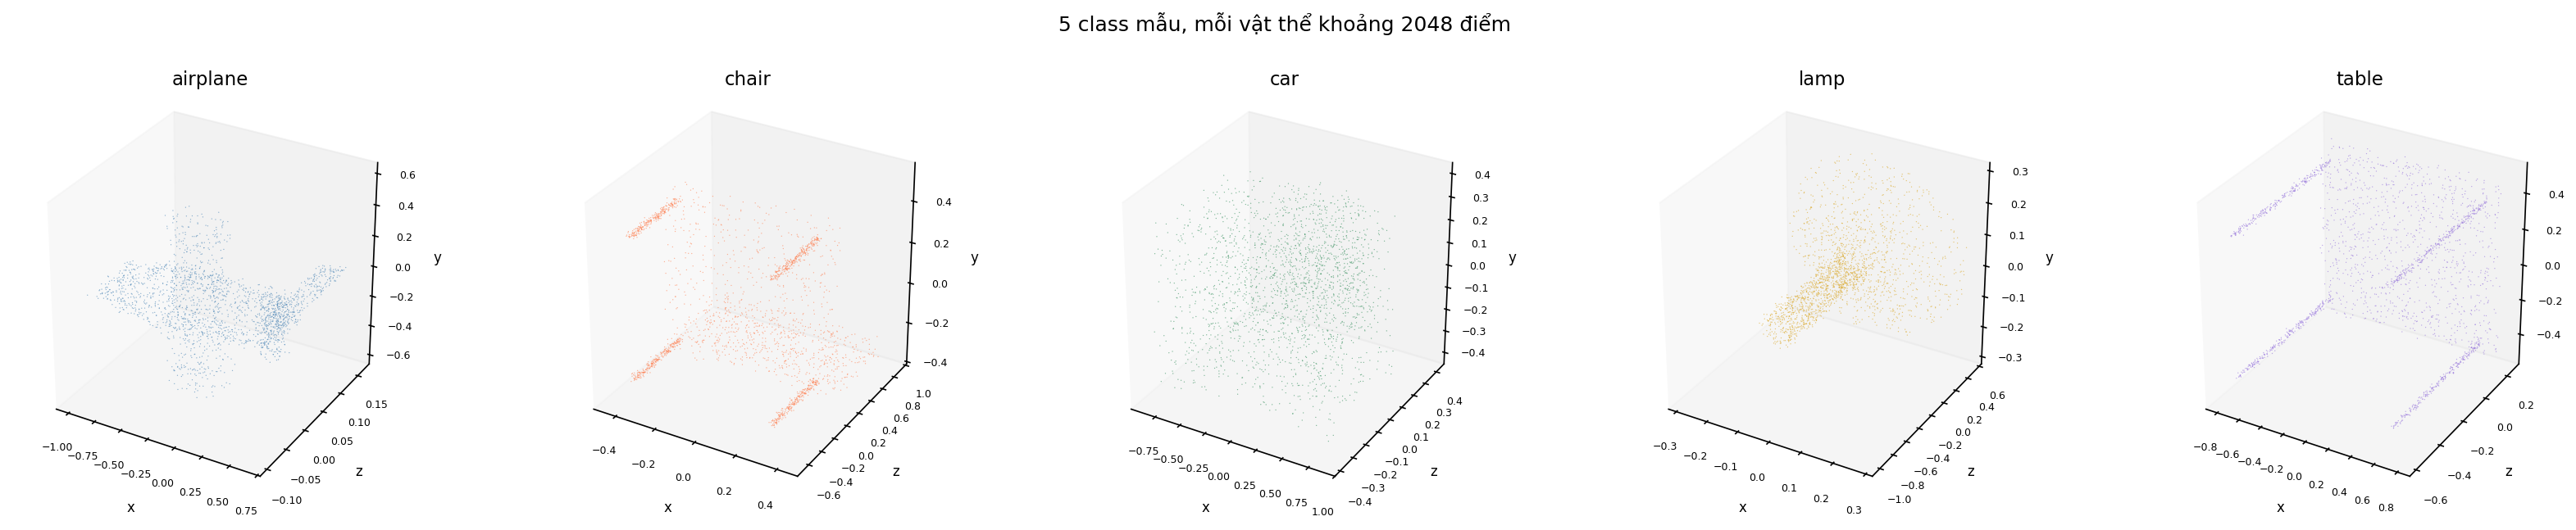
\includegraphics[width=0.78\textwidth]{graphics/point_clouds_5class_2.png}
\caption{Năm lớp point cloud được sử dụng trong demo Part 2.}
\label{fig:demo-point-clouds-5class}
\end{figure}

\subsubsection{Hai biến thể PointNet được so sánh}

\texttt{PointNetBasic} triển khai ý tưởng cốt lõi của PointNet: áp dụng shared MLP lên từng điểm độc lập, sau đó dùng global max pooling để gom toàn bộ tập điểm thành một vector đặc trưng toàn cục. Công thức tổng quát có thể viết dưới dạng:
\begin{equation}
    f(\{x_1,\ldots,x_n\}) \approx \gamma\!\left(\max_{i=1}^{n} h(x_i)\right),
    \label{eq:pointnet-approx-demo}
\end{equation}
trong đó $h$ là shared MLP xử lý từng điểm, $\max$ là phép gộp đối xứng theo trục điểm, và $\gamma$ là mạng phân loại phía sau. Vì phép max không phụ thuộc vào thứ tự các điểm, đầu ra của mô hình bất biến với mọi hoán vị của point cloud.

\texttt{PointNetFull} bổ sung hai T-Net. Input T-Net dự đoán ma trận $3\times3$ để căn chỉnh tọa độ đầu vào, còn Feature T-Net dự đoán ma trận $64\times64$ để căn chỉnh không gian đặc trưng. Khi huấn luyện, mô hình sử dụng thêm ràng buộc trực giao:
\begin{equation}
    \mathcal{L}=\mathcal{L}_{\mathrm{CE}} + \lambda\|I-AA^\top\|_F^2,
    \qquad \lambda=10^{-3},
    \label{eq:pointnet-full-loss-demo}
\end{equation}
trong đó $A$ là ma trận biến đổi do Feature T-Net dự đoán. Trong thiết lập demo, T-Net được giữ ổn định để tránh hiện tượng học không ổn định trên tập nhỏ.

Notebook ghi nhận số tham số của hai mô hình như sau: \texttt{PointNetBasic} có 810,629 tham số, còn \texttt{PointNetFull} có 3,471,054 tham số. Phần chênh lệch 2,660,425 tham số chủ yếu đến từ hai mạng T-Net.

\subsubsection{Thiết lập huấn luyện và kết quả}

Hai mô hình được huấn luyện trong 30 epoch trên tập 5 lớp. \texttt{PointNetBasic} đạt validation accuracy tốt nhất 100.0\% từ epoch 5 và duy trì ổn định trong các lần đánh giá sau. \texttt{PointNetFull} cũng đạt validation accuracy tốt nhất 100.0\%, nhưng đường huấn luyện dao động mạnh hơn ở một vài epoch giữa, ví dụ validation accuracy giảm xuống 80.0\% tại epoch 15 trước khi phục hồi. Điều này phù hợp với trực giác rằng mô hình lớn hơn không nhất thiết ổn định hơn trên tập dữ liệu nhỏ.

\begin{figure}[H]
\centering
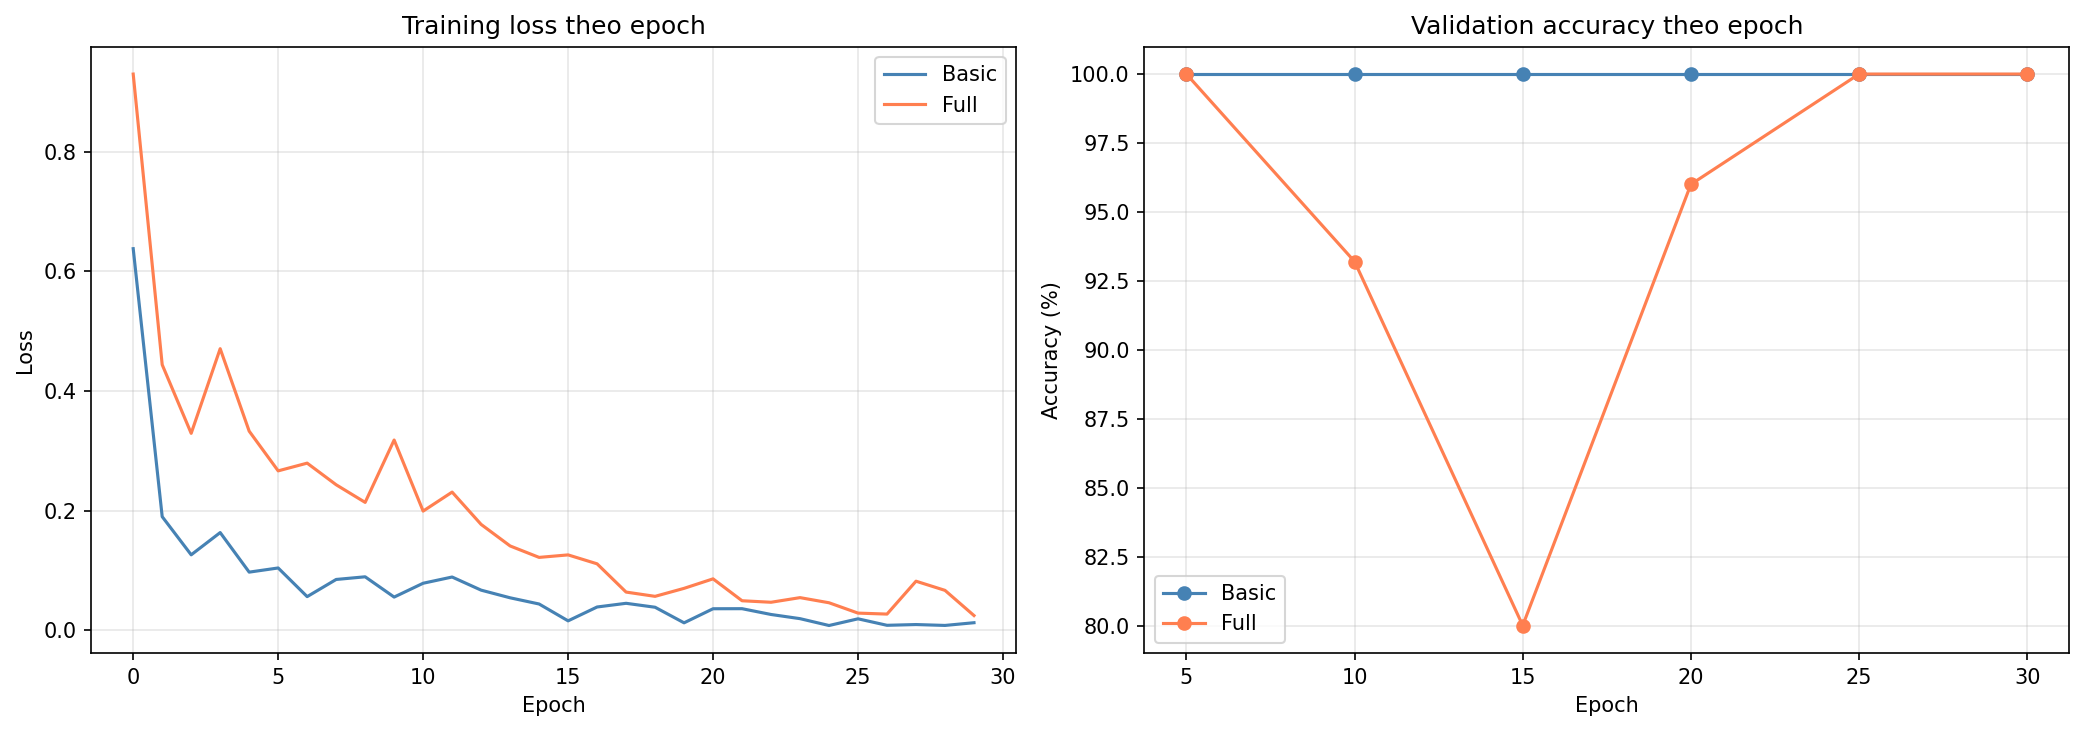
\includegraphics[width=0.82\textwidth]{graphics/training_curves_2.png}
\caption{Đường cong huấn luyện của hai biến thể PointNet trên tập 5 lớp.}
\label{fig:demo-pointnet-training-curves}
\end{figure}

\begin{table}[H]
\centering
\small
\renewcommand{\arraystretch}{1.3} % Tăng lên 1.3 để các dòng có khoảng cách thoáng hơn
% Sử dụng tabularx với tổng chiều rộng \textwidth
% Cột X sẽ tự động tính toán độ rộng còn lại. >{\raggedright\arraybackslash} giúp căn trái cột này một cách tự nhiên.
\begin{tabularx}{\textwidth}{@{} l c c >{\raggedright\arraybackslash}X @{}}
\toprule
\textbf{Mô hình} & \textbf{Số tham số} & \textbf{Best validation accuracy} & \textbf{Nhận xét} \\
\midrule
PointNetBasic & 810,629 & 100.0\% & Nhẹ hơn, hội tụ nhanh và ổn định trên tập nhỏ \\
PointNetFull  & 3,471,054 & 100.0\% & Nhiều tham số hơn, có T-Net, dao động lớn hơn ở giữa quá trình train \\
\bottomrule
\end{tabularx}
\caption{Kết quả huấn luyện hai biến thể PointNet.}
\label{tab:demo-part2-results}
\end{table}

Kết quả 100.0\% cần được hiểu đúng trong phạm vi demo: tập dữ liệu chỉ gồm 5 lớp có hình dạng khác biệt rõ và được tạo ra nhằm phục vụ minh họa tương tác. Vì vậy, con số này không nên được diễn giải như kết quả đại diện cho toàn bộ ModelNet40. Điểm quan trọng của demo nằm ở việc kiểm chứng tính bất biến hoán vị, cơ chế critical points và khả năng bền vững trước perturbation.

\subsubsection{Kiểm tra tính bất biến hoán vị}

Một kiểm tra trực tiếp được thực hiện trong notebook là xáo trộn thứ tự điểm đầu vào 10 lần liên tiếp và so sánh logits của \texttt{PointNetFull}. Kết quả cho thấy cả 10 lần shuffle đều cho logits giống nhau trong sai số tính toán. Đây là minh chứng thực nghiệm cho bất biến hoán vị: thứ tự lưu trữ point cloud không làm thay đổi dự đoán, vì kiến trúc chỉ dùng shared MLP và max pooling trên tập điểm.

\begin{table}[H]
\centering
\small
\begin{tabular}{lc}
\toprule
\textbf{Kiểm tra} & \textbf{Kết quả} \\
\midrule
Số lần shuffle thứ tự điểm & 10 \\
Logits giữ nguyên sau mỗi lần shuffle & True \\
Kết luận & Mô hình bất biến với hoán vị điểm \\
\bottomrule
\end{tabular}
\caption{Kết quả kiểm tra tính bất biến hoán vị của PointNetFull.}
\label{tab:pointnet-permutation-test}
\end{table}

\subsubsection{Robustness và critical points}

Demo hỗ trợ ba dạng perturbation: thay đổi số điểm đầu vào, thêm nhiễu Gaussian và bỏ ngẫu nhiên một tỉ lệ điểm. Các phép thử này giúp quan sát cơ chế mà PointNet sử dụng để tóm tắt hình dạng. Do global max pooling chỉ giữ lại điểm tạo giá trị cực đại ở từng chiều đặc trưng, mô hình thường phụ thuộc vào một tập con nhỏ gồm các điểm có vai trò quyết định, gọi là critical point set.

\begin{figure}[H]
\centering
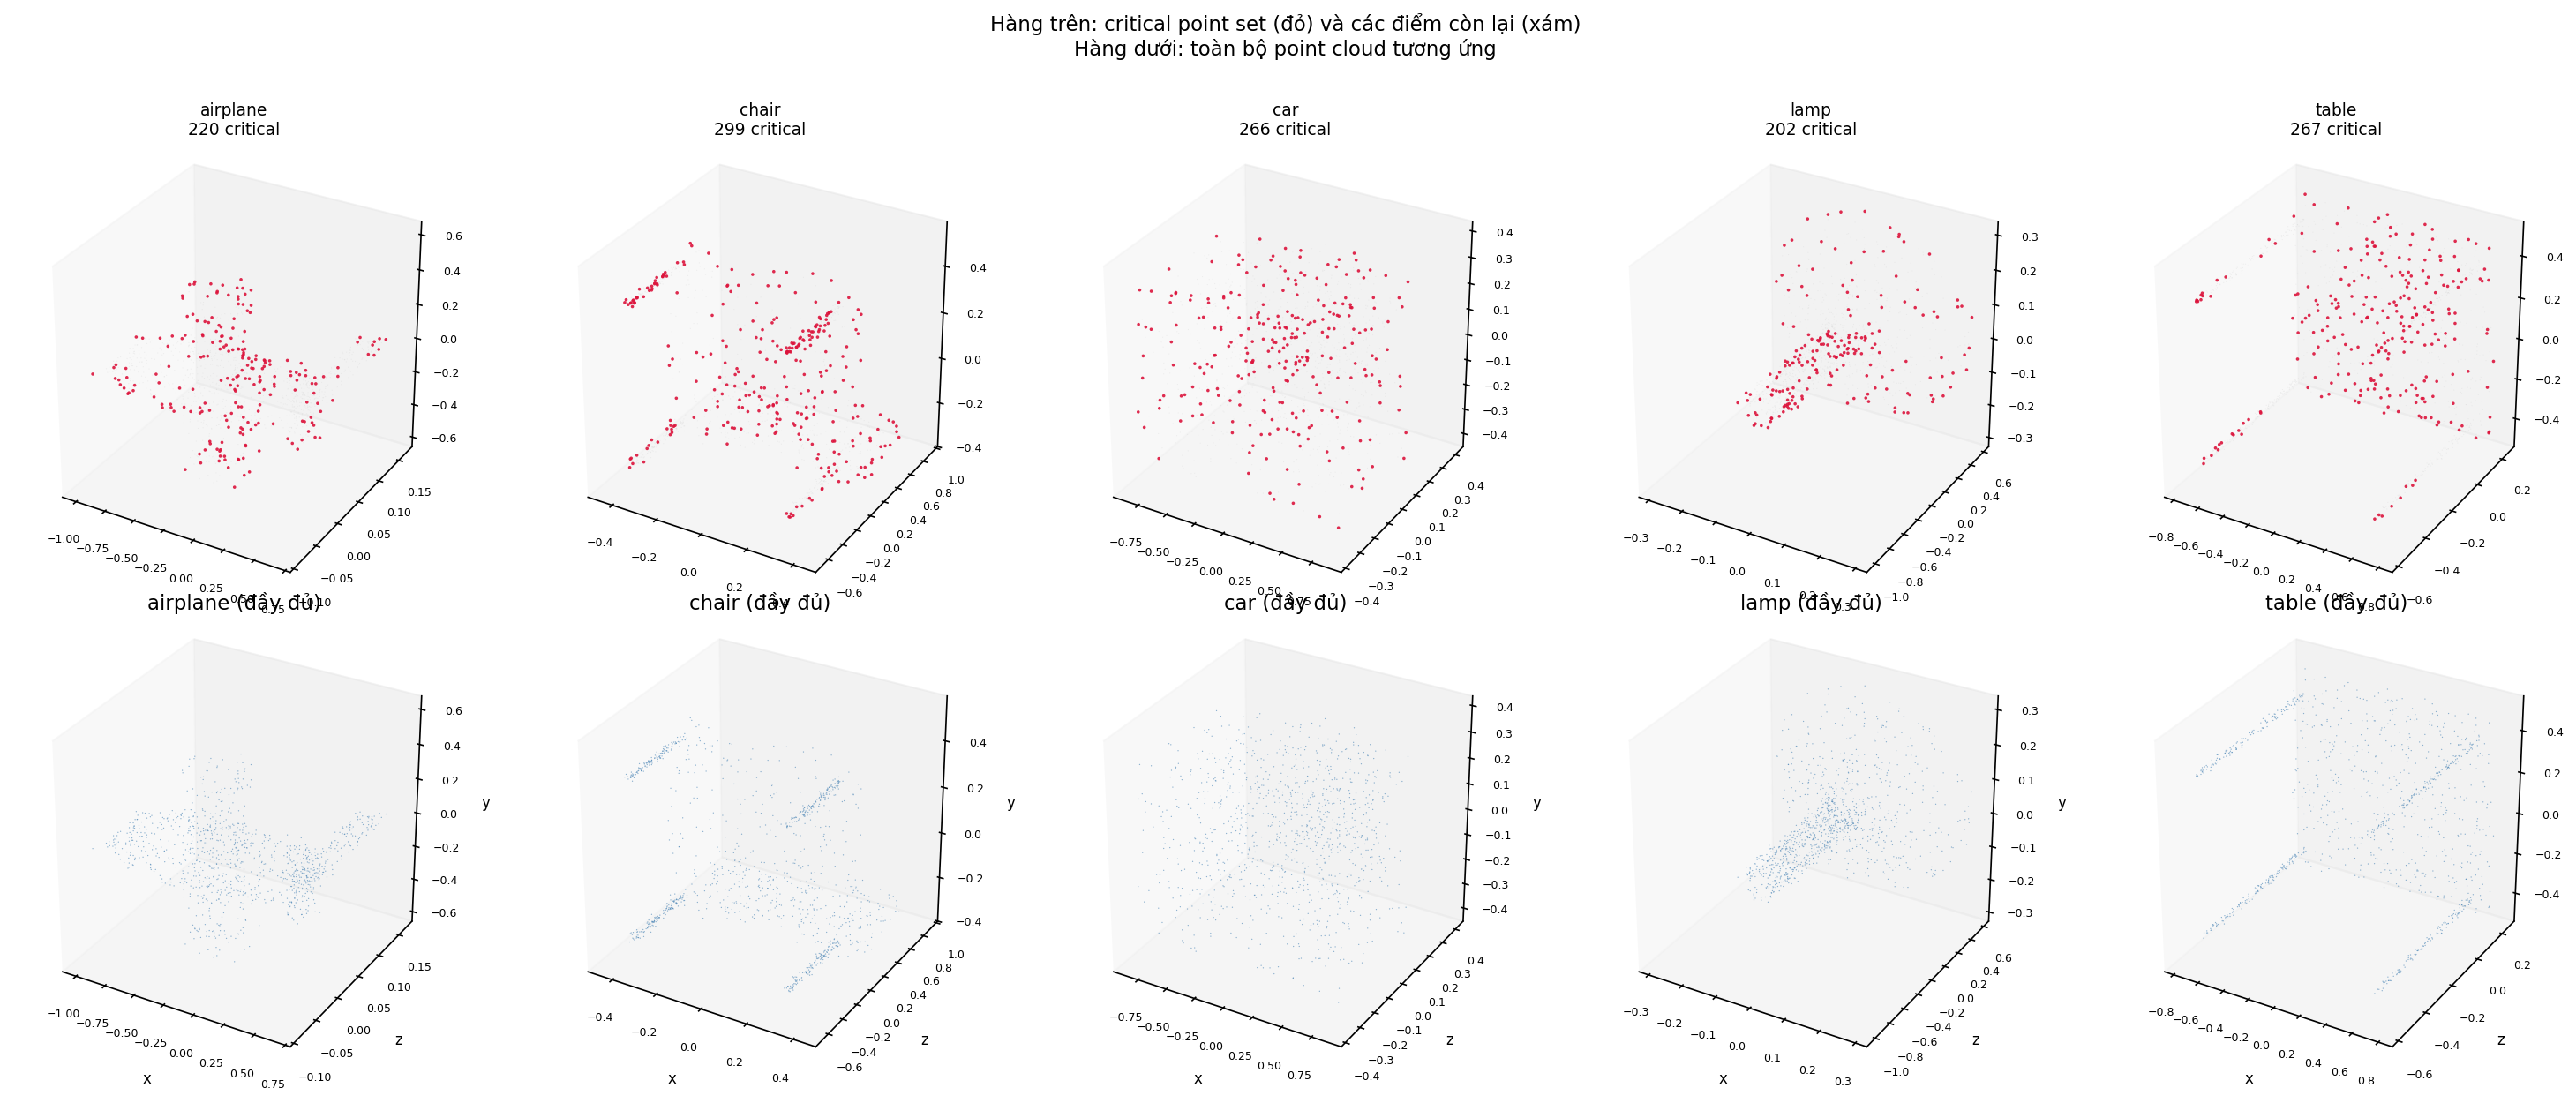
\includegraphics[width=0.82\textwidth]{graphics/critical_points_2.png}
\caption{Minh họa critical points được trích xuất từ PointNet trên point cloud mẫu.}
\label{fig:demo-critical-points}
\end{figure}

Khi người dùng giảm số điểm hoặc bỏ ngẫu nhiên một phần point cloud, mô hình vẫn có thể dự đoán đúng nếu các critical points quan trọng còn được giữ lại. Ngược lại, khi tỉ lệ bỏ điểm quá cao hoặc nhiễu Gaussian làm biến dạng mạnh các vùng biên, đặc trưng toàn cục bị thay đổi và dự đoán bắt đầu kém ổn định. Quan sát này phù hợp với phân tích ở Mục~\ref{sec:pointnet-paper}, trong đó PointNet không ghi nhớ toàn bộ bề mặt vật thể mà học một biểu diễn thưa nhưng có khả năng phân biệt.

\begin{figure}[H]
\centering
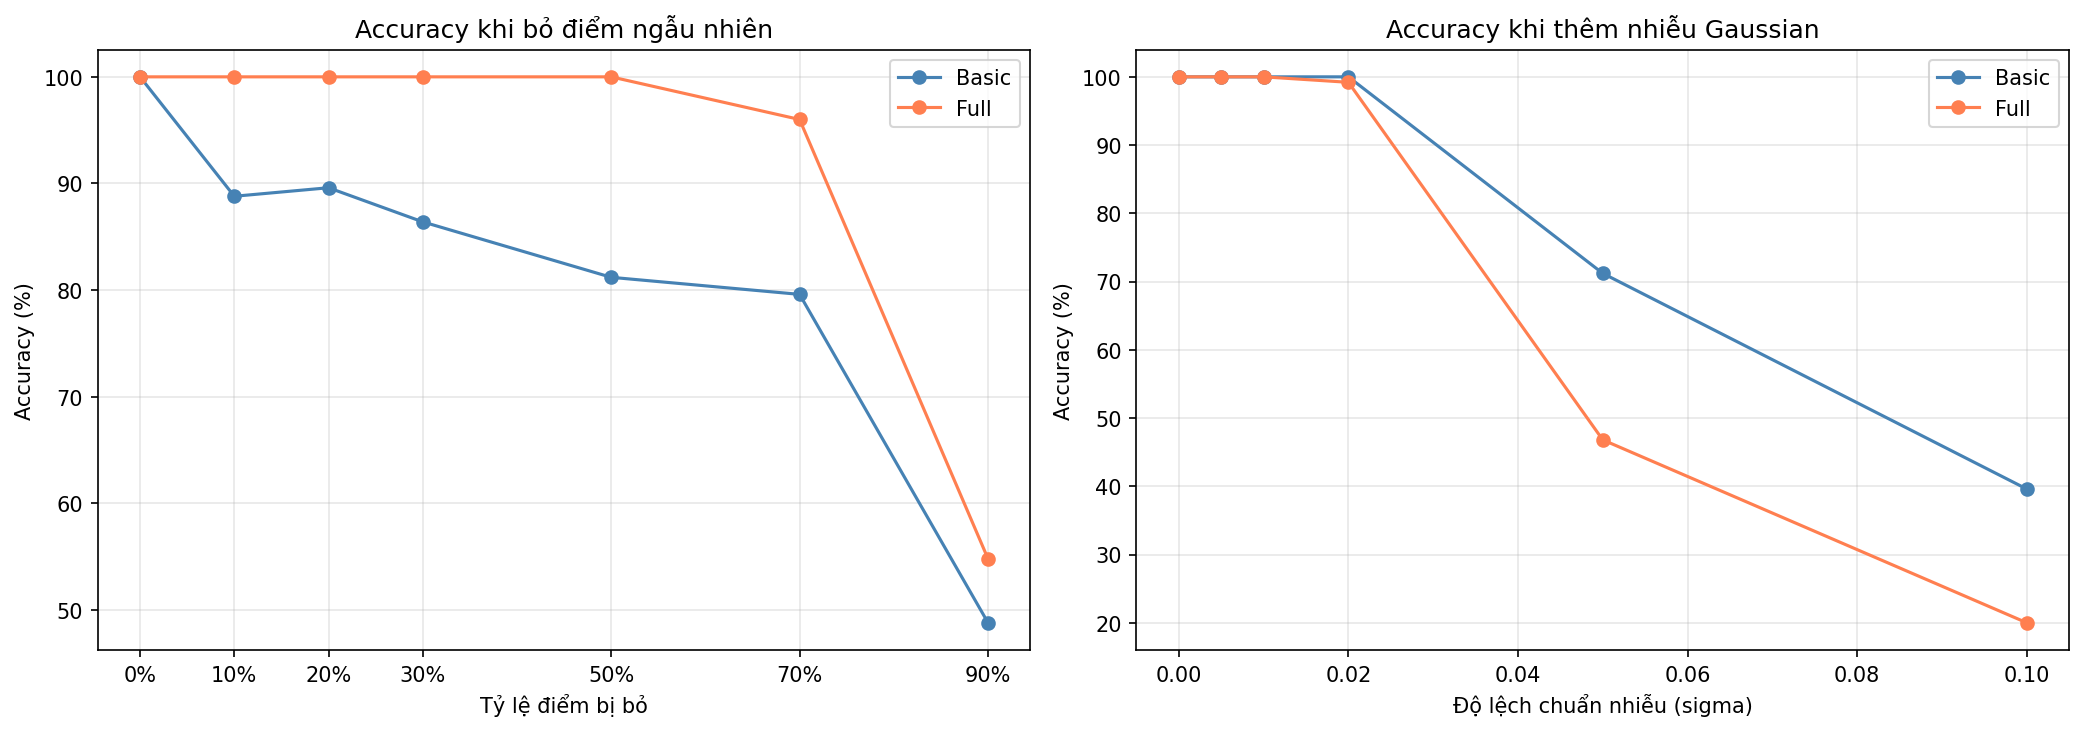
\includegraphics[width=0.82\textwidth]{graphics/robustness_2.png}
\caption{Minh họa xu hướng robustness của PointNet khi point cloud chịu perturbation.}
\label{fig:demo-pointnet-robustness}
\end{figure}

\subsection{Demo thực nghiệm Part 3: Dự đoán năng lượng phân tử với NequIP}
\label{subsec:demo-part3}

Demo thứ ba minh họa bài toán dự đoán năng lượng nội tại $U_0$ của một phân tử cô lập bằng mạng nơ-ron đồ thị đẳng biến $E(3)$. Người dùng chọn một trong bảy phân tử mẫu hoặc tự biên tập tọa độ nguyên tử trong bảng editor, sau đó nhấn nút dự đoán để nhận về giá trị $U_0$ (eV) cùng thời gian inference. Backend xây dựng đồ thị phân tử, chạy NequIP và trả về kết quả qua REST API.

\subsubsection{Bài toán và tính bất biến E(3)}

Năng lượng nội tại $U_0$ là đại lượng vô hướng bất biến với mọi phép biến đổi thuộc nhóm $E(3)$: xoay, phản chiếu và tịnh tiến không làm thay đổi giá trị này. NequIP đảm bảo tính bất biến đó không phải bằng cách học từ dữ liệu, mà bằng cách xây dựng các đặc trưng ẩn \textit{đẳng biến} theo biểu diễn nhóm tương ứng. Khi tổng gộp toàn cục thu gọn các đặc trưng đẳng biến thành một đại lượng vô hướng, tính bất biến $E(3)$ của đầu ra được đảm bảo tự động từ cấu trúc kiến trúc mà không cần học từ dữ liệu.

\subsubsection{Dữ liệu và thiết lập thực nghiệm}

Demo huấn luyện trên tập con của QM9, tập dữ liệu hóa học lượng tử gồm khoảng 134.000 phân tử hữu cơ nhỏ với tối đa 9 nguyên tử nặng (C, N, O, F), tạo thành từ năm nguyên tố H, C, N, O, F. Nhãn $U_0$ của mỗi phân tử được tính bằng lý thuyết phiến hàm mật độ (DFT). Để quan sát hiệu quả dữ liệu, đồ án tạo hai tập con: 100 phân tử và 1000 phân tử. Các tập được chia theo tỉ lệ 80/10/10 (train/validation/test) và được dùng cho checkpoint triển khai trong demo.

\begin{figure}[H]
\centering

\includegraphics[width=0.80\textwidth]{graphics/qm9_molecules_3d.png}
\caption[Bảy phân tử mẫu cài sẵn trong demo Part 3]{Bảy phân tử mẫu cài sẵn trong giao diện demo Part 3.}
\label{fig:demo-part3-molecules}
\vspace{0.15cm}
\begin{minipage}{0.9\linewidth}
    \centering
\end{minipage}
\end{figure}

\vspace{-2.0em}
\noindent\textit{Ghi chú: Bảy cấu trúc gồm $\text{H}_2\text{O}$, $\text{CH}_4$, $\text{NH}_3$, $\text{CO}_2$, $\text{C}_2\text{H}_5\text{OH}$, $\text{CH}_2\text{O}$ và $\text{CH}_3\text{F}$. Fluoromethane là trường hợp thử nghiệm đặc biệt: nếu checkpoint không hỗ trợ nguyên tố F, backend trả về lỗi 422 kèm thông báo rõ ràng thay vì crash server.}

\subsubsection{Kiến trúc NequIP}

NequIP biểu diễn mỗi nguyên tử như một nút trong đồ thị; hai nút $i$ và $j$ được nối bằng cạnh khi khoảng cách $\|\vec{r}_{ij}\| < r_{\max} = 5{,}0\;\text{\AA}$. Đặc trưng cạnh kết hợp phần hướng kính (8 hàm Bessel với hàm cắt đa thức bậc $p = 6$) và phần góc (hàm điều hòa cầu $Y_\ell^m(\hat{r}_{ij})$ đến bậc $\ell_{\max}$). Quá trình message passing qua 4 tầng tương tác dùng tích Clebsch-Gordan để duy trì tính đẳng biến của các irreducible representation xuyên suốt. Sau 4 tầng, từ thành phần vô hướng ($\ell=0$) của mỗi nút, mạng đọc ra một năng lượng nguyên tử riêng; tổng các năng lượng nguyên tử này trên toàn đồ thị cho ra $U_0$.

\begin{table}[H]
\centering
\small
\renewcommand{\arraystretch}{1.3}
\begin{tabular}{@{}p{3.2cm} p{7.4cm} p{3.5cm}@{}}
\toprule
\textbf{Siêu tham số} & \textbf{Ý nghĩa} & \textbf{Giá trị} \\
\midrule
Nguyên tố được hỗ trợ & Tập nguyên tử mô hình nhận được, trùng với 5 nguyên tố trong QM9 & H, C, N, O, F \\
Bán kính cắt $r_{\max}$ & Khoảng cách tối đa để nối cạnh; chỉ các cặp nguyên tử gần hơn ngưỡng này mới tương tác trực tiếp & $5{,}0\;\text{\AA}$ \\
Số tầng tương tác & Số lớp message passing; càng nhiều tầng, thông tin lan truyền càng xa trên đồ thị & 4 \\
$\ell_{\max}$ (cấu hình đẳng biến) & Bậc irreps cao nhất; $\ell_{\max}=1$ cho phép dùng đặc trưng vector có hướng, không chỉ vô hướng & 1 \\
Parity & Cho phép cả irrep chẵn và lẻ, giúp xử lý đúng phép phản chiếu (phân biệt vector và giả vector) & true (cả irrep chẵn và lẻ) \\
Số kênh đặc trưng & Độ rộng vector đặc trưng ẩn ở mỗi nút, quyết định dung lượng biểu diễn của mô hình & 32 \\
Hàm Bessel / bậc cắt $p$ & 8 hàm Bessel mã hóa khoảng cách thành biểu diễn liên tục; envelope đa thức bậc 6 làm đặc trưng cạnh tắt mượt về 0 tại $r_{\max}$ & 8 / 6 \\
Radial MLP & Mạng sinh trọng số phụ thuộc khoảng cách cho tích tensor, điều khiển cường độ tương tác theo $r$ & 2 tầng ẩn, 64 đơn vị \\
EMA decay & Trung bình động hàm mũ của trọng số, làm mượt và ổn định mô hình ở giai đoạn cuối & $0{,}999$ \\
Optimizer / learning rate & Thuật toán tối ưu adaptive với tốc độ học ban đầu & Adam / $5{\times}10^{-3}$ \\
LR scheduler & Giảm tốc độ học $\times 0{,}6$ khi val loss không cải thiện sau 10 epoch & ReduceLROnPlateau (factor $0{,}6$, patience 10) \\
Max epoch / early stopping & Huấn luyện tối đa 200 epoch, dừng sớm nếu val MAE không cải thiện sau 30 epoch & 200 / patience 30 \\
\bottomrule
\end{tabular}
\caption{Siêu tham số của mô hình NequIP triển khai trong demo Part 3.}
\label{tab:demo-part3-arch}
\end{table}
\subsubsection{Luồng inference trong demo}

Khi người dùng nhấn nút dự đoán, frontend gửi danh sách \texttt{(atomic\_numbers, positions)} đến endpoint \texttt{/api/part3/predict-energy}. Backend thực hiện tuần tự: (1) xây dựng đối tượng \texttt{ASE Atoms} không tuần hoàn, (2) áp dụng \texttt{ChemicalSpeciesToAtomTypeMapper} để ánh xạ số nguyên tử sang chỉ số loại trong mô hình, (3) xây dựng danh sách lân cận trong bán kính $r_{\max}$ bằng \texttt{NeighborListTransform}, (4) chạy forward pass qua NequIP và trả về $U_0$ (eV). Toàn bộ pipeline chạy trên CPU với thời gian inference dưới 200 ms cho phân tử có ít hơn 10 nguyên tử.

% Cần: \usepackage{tikz}  \usetikzlibrary{positioning, arrows.meta}
\begin{figure}[H]
\centering
\resizebox{\textwidth}{!}{%

\begin{tikzpicture}[
  box/.style={rectangle, rounded corners=3pt, draw=black!40, line width=0.4pt,
              minimum width=1.9cm, minimum height=1.3cm, align=center,
              text=white, font=\scriptsize\bfseries},
  arr/.style={-{Stealth[length=2mm]}, line width=0.6pt, draw=black!55},
  lbl/.style={font=\tiny, text=black!70, align=center}
]
\node[box, fill=blue!55]                              (edit) {Molecule\\Editor\\(Frontend)};
\node[box, fill=orange!75, right=1.7cm of edit]       (ase)  {ASE\\Atoms};
\node[box, fill=purple!50, right=2.0cm of ase]        (graph){Neighbor\\Graph\\($r<5{,}0$\,\AA)};
\node[box, fill=green!50!black!75, right=1.7cm of graph](gnn) {NequIP GNN\\4 layers, $\ell=1$\\E(3)-equivariant};
\node[box, fill=magenta!60, right=1.7cm of gnn]       (out)  {Energy $U_0$\\(eV)};

\draw[arr] (edit)  -- node[lbl, above]{$Z$, pos}                       (ase);
\draw[arr] (ase)   -- node[lbl, above]{SpeciesToType\\+ NeighborList}  (graph);
\draw[arr] (graph) -- node[lbl, above]{Equivariant\\message passing}   (gnn);
\draw[arr] (gnn)   -- node[lbl, above]{Global\\sum pool}               (out);
\end{tikzpicture}}
\caption{Luồng chuyển đổi từ dữ liệu người dùng nhập vào đến đầu ra năng lượng $U_0$.}
\label{fig:demo-part3-flow}
\end{figure}

\subsubsection{So sánh bất biến và đẳng biến: hiệu quả dữ liệu}

Hai cấu hình được so sánh trên hai kích thước tập dữ liệu. \textit{Baseline} ($\ell_{\max}=0$) chỉ dùng đặc trưng vô hướng, bất biến $E(3)$ theo thiết kế nhưng thiếu thông tin hướng trong các biểu diễn ẩn. \textit{NequIP} ($\ell_{\max}=1$) bổ sung đặc trưng vector, cho phép mạng học các tương tác có hướng như liên kết cộng hóa trị và hiệu ứng cảm ứng.




\begin{figure}[H]
\centering
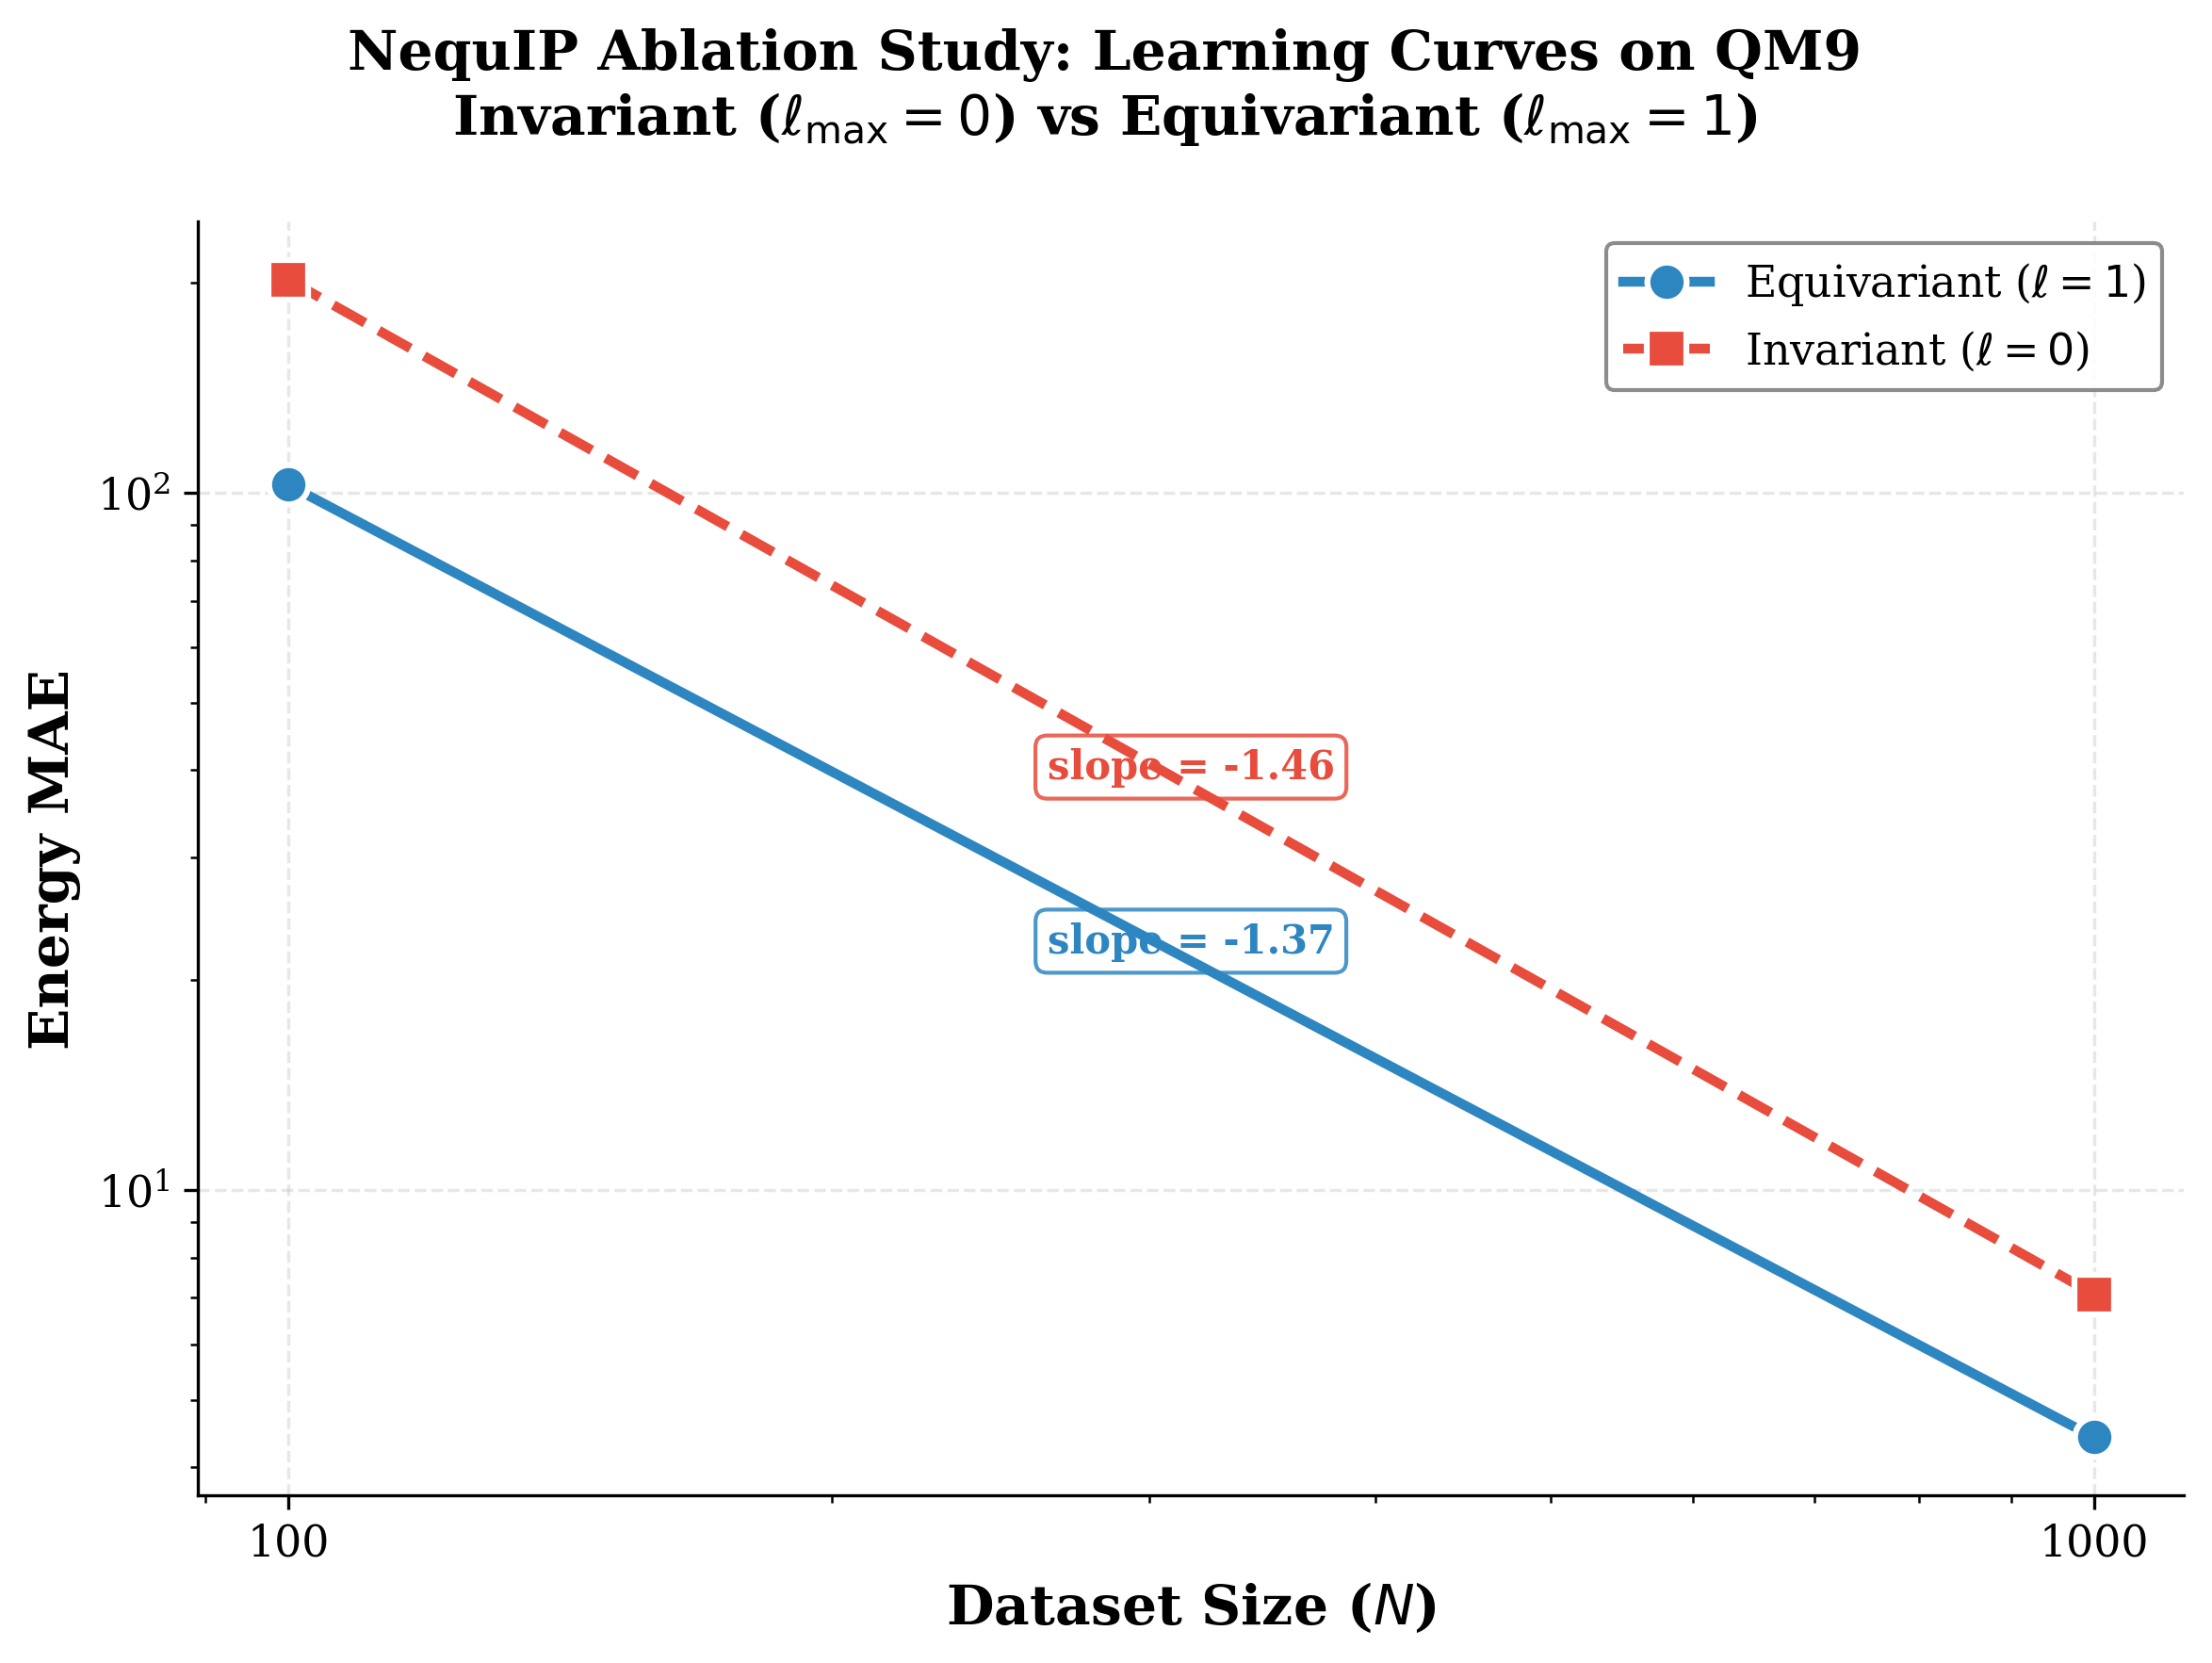
\includegraphics[width=0.82\textwidth]{graphics/nequip_learning_curve.png}
\caption[Đường học log-log của hai cấu hình NequIP trên QM9]{So sánh đường học của Baseline ($\ell_{\max}=0$) và NequIP ($\ell_{\max}=1$) trên hai kích thước tập dữ liệu.}
\label{fig:demo-part3-learning-curve}
\vspace{0.15cm}
\begin{minipage}{0.9\linewidth}
    \centering
\end{minipage}
\end{figure}

\vspace{-2.0em}
\noindent\textit{Ghi chú: Trục x là kích thước tập dữ liệu theo thang log; trục y là MAE năng lượng theo thang log.}

\begin{tcolorbox}[
  enhanced, breakable,
  colback=yellow!12!white,
  colframe=orange!85!black,
  coltitle=black,
  colbacktitle=yellow!55!orange,
  fonttitle=\bfseries,
  title=Nhận xét,
  boxrule=0.8pt, arc=2pt,
  left=2mm, right=2mm, top=1.5mm, bottom=1.5mm
]
\begin{itemize}[leftmargin=1.4em, itemsep=3pt, topsep=2pt]
  \item \textbf{Đẳng biến luôn tốt hơn:} Đường $\ell_{\max}=1$ nằm dưới đường $\ell_{\max}=0$ ở cả $N=100$ và $N=1000$, xác nhận lợi thế của việc mã hóa thông tin hướng qua hàm điều hòa cầu bậc~1.
  \item \textbf{Hiệu quả dữ liệu:} Khoảng cách giữa hai đường lớn hơn ở vùng $N$ nhỏ. Khi dữ liệu ít, việc cài sẵn đối xứng vật lý vào kiến trúc giúp mô hình đạt sai số thấp mà không cần nhiều mẫu huấn luyện.
  \item \textbf{Về độ dốc (slope log-log):} Mô hình bất biến dốc hơn ($-1{,}46$ so với $-1{,}37$), tức cải thiện theo dữ liệu nhanh hơn một chút; nhưng mô hình đẳng biến luôn xuất phát từ MAE thấp hơn nên vẫn tốt hơn ở mọi quy mô. Lợi thế chính của tính đẳng biến nằm ở mức sai số nền, không phải tốc độ scale.
  \item \textbf{Ý nghĩa thang log-log:} Đường thẳng trên trục log-log ứng với quan hệ lũy thừa $\text{MAE} \propto N^{\alpha}$, với $\alpha$ là slope; slope càng âm thì MAE giảm càng nhanh khi tăng dữ liệu.
\end{itemize}
\end{tcolorbox}

\begin{figure}[H]
\centering
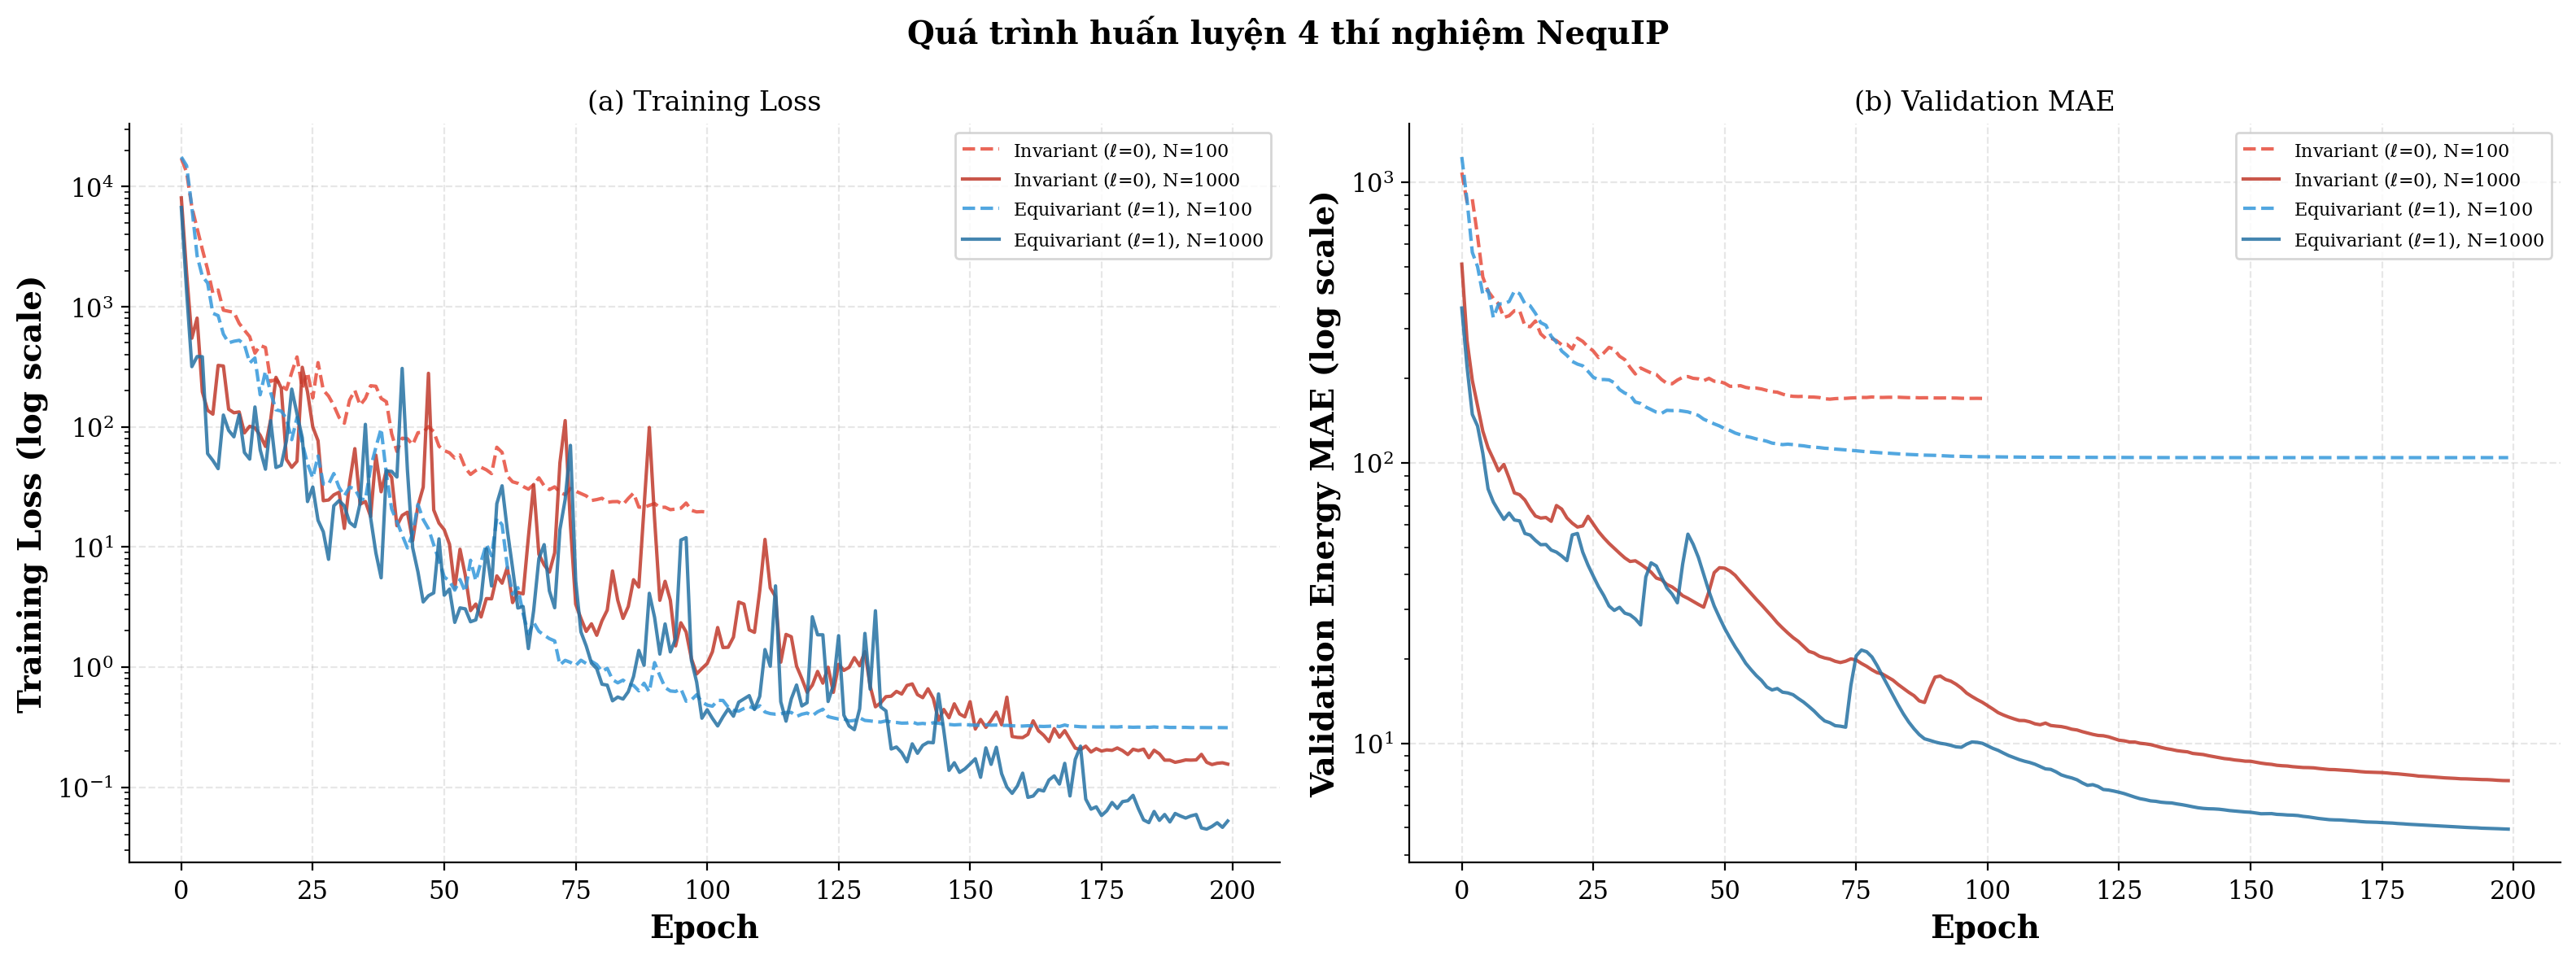
\includegraphics[width=0.95\textwidth]{graphics/nequip_training_curves.png}
\caption[Đường cong huấn luyện bốn thí nghiệm NequIP]{Đường cong training loss (a) và validation MAE (b) theo epoch cho bốn thí nghiệm: bất biến ($\ell_{\max}=0$) và đẳng biến ($\ell_{\max}=1$) trên hai kích thước tập dữ liệu $N=100$ và $N=1000$.}
\label{fig:demo-part3-training}
\end{figure}

\noindent\textit{Ghi chú: Early stopping kích hoạt khi validation MAE không cải thiện trong 30 epoch liên tiếp. EMA (ema\_decay $= 0{,}999$) ổn định quá trình tối ưu hóa ở giai đoạn cuối.}

\begin{tcolorbox}[
  enhanced, breakable,
  colback=blue!5!white,
  colframe=blue!55!black,
  coltitle=white,
  fonttitle=\bfseries,
  title=Nhận xét,
  boxrule=0.8pt, arc=2pt,
  left=2mm, right=2mm, top=1.5mm, bottom=1.5mm
]
\begin{itemize}[leftmargin=1.4em, itemsep=3pt, topsep=2pt]
  \item \textbf{(a) Training loss:} Cả bốn mô hình đều hội tụ. Ở cùng kích thước dữ liệu, loss của $\ell_{\max}=1$ giảm nhanh hơn $\ell_{\max}=0$ trong giai đoạn đầu, cho thấy tính đẳng biến giúp tối ưu hàm mất mát hiệu quả hơn.
  \item \textbf{(b) Validation MAE:} Trong khoảng epoch 0--50, mô hình $\ell_{\max}=1$ giảm MAE nhanh và rõ rệt hơn; sau khi hội tụ, khoảng cách giữa các mô hình thu hẹp lại.
  \item \textbf{Ảnh hưởng kích thước dữ liệu:} Các đường nét đứt ($N=100$, 10 phân tử validation) dao động mạnh hơn, trong khi nét liền ($N=1000$, 100 phân tử validation) mượt và ổn định hơn.
  \item \textbf{Cơ chế ổn định:} Mô hình $N=1000$ cần nhiều epoch hơn để ổn định do tập huấn luyện lớn hơn; early stopping (patience 30) và EMA ($0{,}999$) giúp tránh overfitting và làm mượt giai đoạn cuối.
\end{itemize}
\end{tcolorbox}

\subsection{Thảo luận chung và liên kết lý thuyết}
\label{subsec:thao-luan-thuc-nghiem}

\subsubsection{Tính bất biến xấp xỉ và tính bất biến do kiến trúc}

Ba demo cho thấy ba cách khác nhau để đưa inductive bias hình học vào mô hình. Trong Part 1, Augmented CNN học tính bất biến từ dữ liệu, nên tính bất biến chỉ là xấp xỉ và có thể thất bại ở các trường hợp nhãn mơ hồ. Frame Averaging CNN đưa cấu trúc frame vào bước suy luận, nhờ đó có cơ chế xử lý xoay rõ ràng hơn. Trong Part 2, tính bất biến với hoán vị không cần học từ dữ liệu: nó xuất hiện trực tiếp từ thiết kế shared MLP và max pooling. Trong Part 3, tính bất biến $E(3)$ của đầu ra được đảm bảo qua lý thuyết biểu diễn nhóm: các đặc trưng ẩn đẳng biến theo irreducible representation, và phép tổng gộp toàn cục tự động kết nạp tính bất biến mà không cần bất kỳ xử lý hậu kỳ nào.

\subsubsection{Hiệu quả dữ liệu và giới hạn của demo}

Các kết quả trong chương này cần được hiểu như minh họa thực nghiệm cho lý thuyết, không phải benchmark đầy đủ trên quy mô lớn. Part 1 dùng MNIST để làm rõ ảnh hưởng của phép xoay trong môi trường dễ quan sát. Part 2 dùng 5 lớp trích từ ModelNet40 để giao diện demo nhẹ và phản hồi nhanh. Part 3 dùng tập con 1000 phân tử của QM9 để minh họa lợi ích của đẳng biến $E(3)$ trên dữ liệu phân tử thực tế. Giá trị MAE trong Part 3 phản ánh tập huấn luyện nhỏ và không nên so sánh trực tiếp với các kết quả công bố trên toàn bộ QM9.

Dù vậy, xu hướng chung vẫn nhất quán với lý thuyết ở Chương~\ref{sec:phuong-phap}: khi cấu trúc đối xứng được đưa vào mô hình, mô hình cần ít dữ liệu hơn để học cùng một quy luật và có hành vi ổn định hơn trước các biến đổi không làm thay đổi bản chất đối tượng.

\subsubsection{Đối chiếu hai hướng tiếp cận}

\begin{table}[H]
\centering
\small
\renewcommand{\arraystretch}{1.3}
\begin{tabularx}{\textwidth}{p{0.17\textwidth}>{\raggedright\arraybackslash}X>{\raggedright\arraybackslash}X>{\raggedright\arraybackslash}X}
\toprule
\textbf{Tiêu chí} & \textbf{Part 1: MNIST xoay} & \textbf{Part 2: PointNet} & \textbf{Part 3: NequIP} \\
\midrule
Đối tượng dữ liệu & Ảnh $28\times28$ trên lưới 2D & Tập điểm không có thứ tự trong không gian 3D & Phân tử hóa học với tọa độ nguyên tử 3D \\
Nhóm đối xứng & $SO(2)$, phép xoay liên tục & $S_n$, phép hoán vị hữu hạn & $E(3)$, nhóm Euclidean trong $\mathbb{R}^3$ \\
Cách đưa đối xứng vào mô hình & Data augmentation hoặc frame averaging & Shared MLP và max pooling & Equivariant message passing với irrep \\
Loại bất biến & Xấp xỉ với augmentation, rõ ràng hơn với frame averaging & Bất biến hoán vị ngay từ kiến trúc & Bất biến $E(3)$ được đảm bảo bằng biểu diễn nhóm \\
Giới hạn chính & Ambiguity nhãn khi xoay một số chữ số & Demo chỉ dùng 5 lớp, chưa đại diện toàn bộ ModelNet40 & Tập huấn luyện nhỏ (1000 phân tử), chưa tính lực \\
\bottomrule
\end{tabularx}
\caption{Đối chiếu ba demo thực nghiệm qua lăng kính ba hướng tiếp cận geometric machine learning.}
\label{tab:demo-lien-ket}
\end{table}

Từ ba demo, có thể rút ra kết luận rằng inductive bias hình học không chỉ giúp tăng độ chính xác trong một số thiết lập, mà quan trọng hơn là làm cho hành vi của mô hình nhất quán hơn với cấu trúc của dữ liệu. Với ảnh xoay, mô hình cần hiểu quan hệ giữa các góc. Với point cloud, mô hình cần bỏ qua thứ tự lưu trữ điểm. Với phân tử hóa học, mô hình cần đảm bảo rằng xoay hay phản chiếu toàn bộ phân tử không thay đổi năng lượng dự đoán. Ba yêu cầu này tương ứng với ba cơ chế khác nhau để tích hợp đối xứng vào học máy, và đây chính là vai trò trung tâm của geometric machine learning: thiết kế mô hình không chỉ dựa trên dữ liệu đầu vào, mà còn dựa trên những phép biến đổi mà bài toán cho phép hoặc cần bất biến theo.

\clearpage


\clearpage

\phantomsection
\addcontentsline{toc}{section}{Tài liệu tham khảo}
\bibliographystyle{IEEEtran}
\bibliography{refs/references.bib}
\nocite{*}

\end{document}
